\documentclass[12pt, a4paper]{report}
\usepackage{natbib}
\usepackage{vmargin}
\usepackage{graphicx}
\usepackage{epsfig}
\usepackage{subfigure}
%\usepackage{amscd}
\usepackage{amssymb}
\usepackage{framed}
\usepackage{amsbsy}
\usepackage{amsthm, amsmath}
%\usepackage[dvips]{graphicx}
\bibliographystyle{chicago}
\renewcommand{\baselinestretch}{1.8}

% left top textwidth textheight headheight % headsep footheight footskip
\setmargins{3.0cm}{2.5cm}{15.5 cm}{23.5cm}{0.5cm}{0cm}{1cm}{1cm}

\pagenumbering{arabic}


\begin{document}
\author{Kevin O'Brien}
\title{SCRATCH}
\date{\today}
\maketitle

\tableofcontents \setcounter{tocdepth}{2}
%-------------------------------------------------

\begin{enumerate}
	\item Agreement and Method Comparison Studies
	\begin{enumerate}
		\item What is Agreement?
		\item Repeatability
		\item
		\item
		\item
	\end{enumerate}
	\item Bland Altman Single Observations
	\begin{enumerate}
		\item
		\item
	\end{enumerate}
	\item Alternative Methods
	\begin{enumerate}
		\item Deming Regression
		\item Mountain Plot
		\item Bartko's Ellipse
		\item Formal Tests and Procedures
	\end{enumerate}
	\item Replicate Observations
	
	\item LME models
	
	\item Estimation and Algorithms
	\begin{enumerate}
		\item ML and REML estimation
		\item MINQUE
		\item
	\end{enumerate}
	\item Residual Diagnostics
	\begin{enumerate}
		\item Marginal and Conditional Diagnostics
		\item Scaled Residuals
	\end{enumerate}
	
	\item Influence Diagnostics
	\begin{enumerate}
		\item Underlying Concepts
		\item Managing the Covariance Parameters
		\item Predicted Values, PRESS Residual and the PRESS Statistic
		\item Leverage
		\item Internally and Externally Studentized Residuals
		\item DFFITs and MDFFITs
		\item Covariance Ratio and Trace
		\item Likelihood Distance
		\item Non-iterative Update Procedures
	\end{enumerate}
\end{enumerate}
\newpage
	\chapter{Introduction}
	
	\section{Introduction}
	The problem of assessing the agreement between two or more methods
	of measurement is ubiquitous in scientific research, and is
	commonly referred to as a `method comparison study'. Published
	examples of method comparison studies can be found in disciplines
	as diverse as Pharmacology \citep{ludbrook97}, Anaesthesia
	\citep{Myles}, and cardiac imaging methods \citep{Krumm}.
	\smallskip
	
	To illustrate the characteristics of a typical method comparison
	study consider the data in Table I \citep{Grubbs73}. In each of
	twelve experimental trials a single round of ammunition was fired
	from a 155mm gun, and its velocity was measured simultaneously
	(and independently) by three chronographs devices, identified here
	by the labels `Fotobalk', `Counter' and `Terma'.
	\smallskip
	
	
	\newpage
	
	\begin{table}[ht]
		\begin{center}
			\begin{tabular}{rrrr}
				\hline
				Round& Fotobalk [F] & Counter [C]& Terma [T]\\
				\hline
				1 & 793.8 & 794.6 & 793.2 \\
				2 & 793.1 & 793.9 & 793.3 \\
				3 & 792.4 & 793.2 & 792.6 \\
				4 & 794.0 & 794.0 & 793.8 \\
				5 & 791.4 & 792.2 & 791.6 \\
				6 & 792.4 & 793.1 & 791.6 \\
				7 & 791.7 & 792.4 & 791.6 \\
				8 & 792.3 & 792.8 & 792.4 \\
				9 & 789.6 & 790.2 & 788.5 \\
				10 & 794.4 & 795.0 & 794.7 \\
				11 & 790.9 & 791.6 & 791.3 \\
				12 & 793.5 & 793.8 & 793.5 \\
				\hline
			\end{tabular}
			\caption{Velocity measurement from the three chronographs (Grubbs
				1973).}
		\end{center}
	\end{table}
	
	An important aspect of the these data is that all three methods of
	measurement are assumed to have an attended measurement error, and
	the velocities reported in Table 1.1 can not be assumed to be
	`true values' in any absolute sense.
	
	%While lack of
	%agreement between two methods is inevitable, the question , as
	%posed by \citet{BA83}, is 'do the two methods of measurement agree
	%sufficiently closely?'
	
	A method of measurement should ideally be both accurate and
	precise. \citet{Barnhart} describes agreement as being a broader
	term that contains both of those qualities. An accurate
	measurement method will give results close to the unknown `true
	value'. The precision of a method is indicated by how tightly
	measurements obtained under identical conditions are distributed
	around their mean measurement value. A precise and accurate method
	will yield results consistently close to the true value. Of course
	a method may be accurate, but not precise. If the average of its
	measurements is close to the true value, but those measurements
	are highly dispersed. Conversely a method that is not accurate may
	be quite precise, as it consistently indicates the same level of
	inaccuracy. The tendency of a method of measurement to
	consistently give results above or below the true value is a
	source of systematic bias. The smaller the systematic bias, the
	greater the accuracy of the method.
	
	
	The FDA define precision as the closeness of agreement (degree of
	scatter) between a series of measurements obtained from multiple
	sampling of the same homogeneous sample under prescribed
	conditions. \citet{Barnhart} describes precision as being further
	subdivided as either within-run, intra-batch precision or
	repeatability (which assesses precision during a single analytical
	run), or between-run, inter-batch precision or repeatability
	(which measures precision over time)
	
	In the context of the agreement of two methods, there is also a
	tendency of one measurement method to consistently give results
	above or below the other method. Lack of agreement is a
	consequence of the existence of `inter-method bias'. For two
	methods to be considered in good agreement, the inter-method bias
	should be in the region of zero. A simple estimation of the
	inter-method bias can be calculated using the differences of the
	paired measurements. The data in Table 1.2 are a good example of
	possible inter-method bias; the `Fotobalk' consistently recording
	smaller velocities than the `Counter' method. Consequently one
	would conclude that there is lack of agreement between the two
	methods.
	
	The absence of inter-method bias by itself is not sufficient to
	establish whether two measurement methods agree. The two
	methods must also have equivalent levels of precision. Should one
	method yield results considerably more variable than that of the
	other, they can not be considered to be in agreement. With this in
	mind a methodology is required that allows an analyst to estimate
	the inter-method bias, and to compare the precision of both
	methods of measurement.
	\newpage
	% latex table generated in R 2.6.0 by xtable 1.5-5 package
	% Wed Aug 26 15:22:41 2009
	\begin{table}[h!]
		
		\begin{center}
			
			\begin{tabular}{rrrr}
				\hline
				Round& Fotobalk (F) & Counter (C) & F-C \\
				\hline
				1 & 793.8& 794.6 & -0.8 \\
				2 & 793.1 & 793.9 & -0.8 \\
				3 & 792.4 & 793.2 & -0.8 \\
				4 & 794.0 & 794.0 & 0.0 \\
				5 & 791.4 & 792.2 & -0.8 \\
				6 & 792.4 & 793.1 & -0.7 \\
				7 & 791.7 & 792.4 & -0.7 \\
				8 & 792.3 & 792.8 & -0.5 \\
				9 & 789.6 & 790.2 & -0.6 \\
				10 & 794.4 & 795.0 & -0.6 \\
				11 & 790.9 & 791.6 & -0.7 \\
				12 & 793.5 & 793.8 & -0.3 \\
				\hline
			\end{tabular}
			\caption{Difference between Fotobalk and Counter measurements.}
		\end{center}
	\end{table}
	
	\bigskip
	
	
	%%%%%%%%%%%%%%%%%%%%%%%%%%%%%%%%%%%%%%%%%%%%%%%%%%%%%%%%%%%%%%%%%%%%%%%%%%%%%%%%%%%%%%
	%\newpage
	\section{Introduction}
	The problem of assessing the agreement between two or more methods
	of measurement is ubiquitous in scientific research, and is
	commonly referred to as a `method comparison study'. Published
	examples of method comparison studies can be found in disciplines
	as diverse as Pharmacology \citep{ludbrook97}, Anaesthesia
	\citep{Myles}, and cardiac imaging methods \citep{Krumm}.
	\smallskip
	
	To illustrate the characteristics of a typical method comparison
	study consider the data in Table I \citep{Grubbs73}. In each of
	twelve experimental trials a single round of ammunition was fired
	from a 155mm gun, and its velocity was measured simultaneously
	(and independently) by three chronographs devices, identified here
	by the labels `Fotobalk', `Counter' and `Terma'.
	\smallskip
	
	
	\newpage
	
	\begin{table}[ht]
		\begin{center}
			\begin{tabular}{rrrr}
				\hline
				Round& Fotobalk [F] & Counter [C]& Terma [T]\\
				\hline
				1 & 793.8 & 794.6 & 793.2 \\
				2 & 793.1 & 793.9 & 793.3 \\
				3 & 792.4 & 793.2 & 792.6 \\
				4 & 794.0 & 794.0 & 793.8 \\
				5 & 791.4 & 792.2 & 791.6 \\
				6 & 792.4 & 793.1 & 791.6 \\
				7 & 791.7 & 792.4 & 791.6 \\
				8 & 792.3 & 792.8 & 792.4 \\
				9 & 789.6 & 790.2 & 788.5 \\
				10 & 794.4 & 795.0 & 794.7 \\
				11 & 790.9 & 791.6 & 791.3 \\
				12 & 793.5 & 793.8 & 793.5 \\
				\hline
			\end{tabular}
			\caption{Velocity measurement from the three chronographs (Grubbs
				1973).}
		\end{center}
	\end{table}
	
	An important aspect of the these data is that all three methods of
	measurement are assumed to have an attended measurement error, and
	the velocities reported in Table 1.1 can not be assumed to be
	`true values' in any absolute sense.
	
	%While lack of
	%agreement between two methods is inevitable, the question , as
	%posed by \citet{BA83}, is 'do the two methods of measurement agree
	%sufficiently closely?'
	
	A method of measurement should ideally be both accurate and
	precise. \citet{Barnhart} describes agreement as being a broader
	term that contains both of those qualities. An accurate
	measurement method will give results close to the unknown `true
	value'. The precision of a method is indicated by how tightly
	measurements obtained under identical conditions are distributed
	around their mean measurement value. A precise and accurate method
	will yield results consistently close to the true value. Of course
	a method may be accurate, but not precise. If the average of its
	measurements is close to the true value, but those measurements
	are highly dispersed. Conversely a method that is not accurate may
	be quite precise, as it consistently indicates the same level of
	inaccuracy. The tendency of a method of measurement to
	consistently give results above or below the true value is a
	source of systematic bias. The smaller the systematic bias, the
	greater the accuracy of the method.
	
	
	The FDA define precision as the closeness of agreement (degree of
	scatter) between a series of measurements obtained from multiple
	sampling of the same homogeneous sample under prescribed
	conditions. \citet{Barnhart} describes precision as being further
	subdivided as either within-run, intra-batch precision or
	repeatability (which assesses precision during a single analytical
	run), or between-run, inter-batch precision or repeatability
	(which measures precision over time)
	
	In the context of the agreement of two methods, there is also a
	tendency of one measurement method to consistently give results
	above or below the other method. Lack of agreement is a
	consequence of the existence of `inter-method bias'. For two
	methods to be considered in good agreement, the inter-method bias
	should be in the region of zero. A simple estimation of the
	inter-method bias can be calculated using the differences of the
	paired measurements. The data in Table 1.2 are a good example of
	possible inter-method bias; the `Fotobalk' consistently recording
	smaller velocities than the `Counter' method. Consequently one
	would conclude that there is lack of agreement between the two
	methods.
	
	The absence of inter-method bias by itself is not sufficient to
	establish whether two measurement methods agree. The two
	methods must also have equivalent levels of precision. Should one
	method yield results considerably more variable than that of the
	other, they can not be considered to be in agreement. With this in
	mind a methodology is required that allows an analyst to estimate
	the inter-method bias, and to compare the precision of both
	methods of measurement.
	\newpage
	% latex table generated in R 2.6.0 by xtable 1.5-5 package
	% Wed Aug 26 15:22:41 2009
	\begin{table}[h!]
		
		\begin{center}
			
			\begin{tabular}{rrrr}
				\hline
				Round& Fotobalk (F) & Counter (C) & F-C \\
				\hline
				1 & 793.8& 794.6 & -0.8 \\
				2 & 793.1 & 793.9 & -0.8 \\
				3 & 792.4 & 793.2 & -0.8 \\
				4 & 794.0 & 794.0 & 0.0 \\
				5 & 791.4 & 792.2 & -0.8 \\
				6 & 792.4 & 793.1 & -0.7 \\
				7 & 791.7 & 792.4 & -0.7 \\
				8 & 792.3 & 792.8 & -0.5 \\
				9 & 789.6 & 790.2 & -0.6 \\
				10 & 794.4 & 795.0 & -0.6 \\
				11 & 790.9 & 791.6 & -0.7 \\
				12 & 793.5 & 793.8 & -0.3 \\
				\hline
			\end{tabular}
			\caption{Difference between Fotobalk and Counter measurements.}
		\end{center}
	\end{table}
	
	\bigskip
	
	
	%%%%%%%%%%%%%%%%%%%%%%%%%%%%%%%%%%%%%%%%%%%%%%%%%%%%%%%%%%%%%%%%%%%%%%%%%%%%%%%%%%%%%%
	%\newpage
	\section{Bland-Altman Plots}
	The issue of whether two measurement methods comparable to the
	extent that they can be used interchangeably with sufficient
	accuracy is encountered frequently in scientific research.
	Historically comparison of two methods of measurement was carried
	out by use of paired sample t-test, correlation coefficients or
	simple linear regression. Statisticians Martin Bland and Douglas
	Altman recognized the inadequacies of these analyses and
	articulated quite thoroughly the basis on which of which they are
	unsuitable for comparing two methods of measurement \citep*{BA83}.
	Furthermore they proposed their simple methodology specifically
	constructed for method comparison studies. They acknowledge the
	opportunity to apply other valid, but complex, methodologies, but
	argue that a simple approach is preferable, especially when the
	results must be `explained to non-statisticians'.
	
	Notwithstanding previous remarks about regression, the first step
	recommended, which the authors argue should be mandatory, is
	construction of a simple scatter plot of the data. The line of
	equality should also be shown, as it is necessary to give the
	correct interpretation of how both methods compare. A scatter plot
	of the Grubbs data is shown in Figure 1.1. Visual inspection confirms the previous conclusion that there is an
	inter-method bias present, i.e. Fotobalk device has a tendency to
	record a lower velocity.
	
	\begin{figure}[h!]
		\begin{center}
			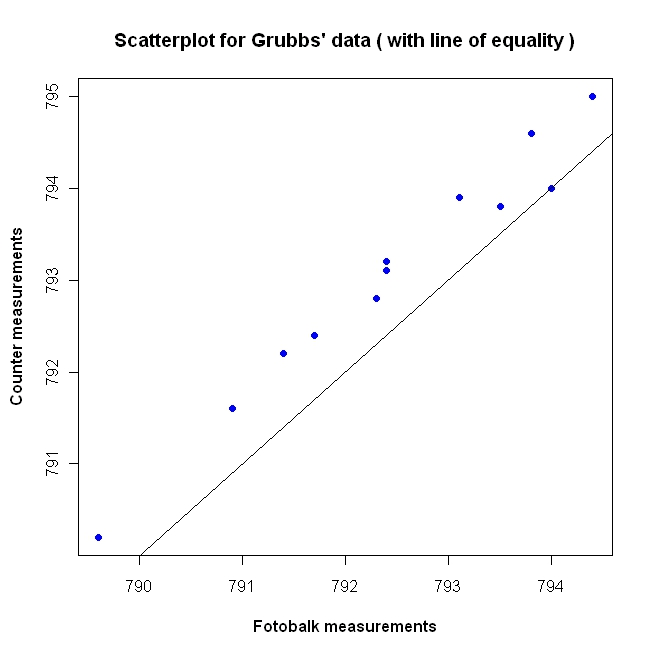
\includegraphics[width=130mm]{images/GrubbsScatter.jpeg}
			\caption{Scatter plot For Fotobalk and Counter Methods.}\label{GrubbsScatter}
		\end{center}
	\end{figure}
	
	In light of shortcomings associated with scatterplots,
	\citet*{BA83} recommend a further analysis of the data. Firstly
	case-wise differences of measurements of two methods $d_{i} =
	y_{1i}-y_{2i} \mbox{ for }i=1,2,..n$ on the same subject should be
	calculated, and then the average of those measurements ($a_{i} =
	(y_{1i} + y_{2i})/2 \mbox{ for }i=1,2,..n$). These differences and
	averages are then plotted. This methodology, now commonly known as
	the `Bland-Altman Plot', has proved very successful.
	\citet*{BA86}, which further develops the methodology, was found
	to be the sixth most cited paper of all time by the
	\citet{BAcite}. \cite{Dewitte} also commented on the rate at which
	prevalence of the Bland-Altman plot has developed in scientific
	literature. The Bland-Altman Plot has since become expected, and
	often obligatory, approach for presenting method comparison
	studies in many scientific journals \citep{hollis}. Furthermore
	\citet{BritHypSoc} recommend its use in papers pertaining to
	method comparison studies for the journal of the British
	Hypertension Society.
	
	The magnitude of the inter-method bias between the two methods is
	simply the average of the differences $\bar{d}$. The variances
	around this bias is estimated by the standard deviation of the
	differences $S(d)$. This inter-method bias is represented with a
	line on the Bland-Altman plot. These estimates are only meaningful
	if there is uniform inter-bias and variability throughout the
	range of measurements, which can be checked by visual inspection
	of the plot. In the case of Grubbs data the inter-method bias is
	$-0.61$ metres per second, and is indicated by the dashed line on
	Figure 1.2. By inspection of the plot, it is also possible to
	compare the precision of each method. Noticeably the differences
	tend to increase as the averages increase.
	
	
	\begin{table}[h!]
		\renewcommand\arraystretch{0.7}%
		\begin{center}
			\begin{tabular}{|c||c|c||c|c|}
				\hline
				Round & Fotobalk  & Counter  & Differences  & Averages  \\
				&  [F] & [C] & [F-C] &  [(F+C)/2] \\
				\hline
				1 & 793.8 & 794.6 & -0.8 & 794.2 \\
				2 & 793.1 & 793.9 & -0.8 & 793.5 \\
				3 & 792.4 & 793.2 & -0.8 & 792.8 \\
				4 & 794.0 & 794.0 & 0.0 & 794.0 \\
				5 & 791.4 & 792.2 & -0.8 & 791.8 \\
				6 & 792.4 & 793.1 & -0.7 & 792.8 \\
				7 & 791.7 & 792.4 & -0.7 & 792.0 \\
				8 & 792.3 & 792.8 & -0.5 & 792.5 \\
				9 & 789.6 & 790.2 & -0.6 & 789.9 \\
				10 & 794.4 & 795.0 & -0.6 & 794.7 \\
				11 & 790.9 & 791.6 & -0.7 & 791.2 \\
				12 & 793.5 & 793.8 & -0.3 & 793.6 \\
				\hline
			\end{tabular}
			\caption{Fotobalk and Counter methods: differences and averages.}
		\end{center}
	\end{table}
	
	\begin{table}[h!]
		\renewcommand\arraystretch{0.7}%
		\begin{center}
			\begin{tabular}{|c||c|c||c|c|}
				\hline
				Round & Fotobalk  & Terma  & Differences  & Averages  \\
				&  [F] & [T] & [F-T] &  [(F+T)/2] \\
				\hline
				1 & 793.80 & 793.20 & 0.60 & 793.50 \\
				2 & 793.10 & 793.30 & -0.20 & 793.20 \\
				3 & 792.40 & 792.60 & -0.20 & 792.50 \\
				4 & 794.00 & 793.80 & 0.20 & 793.90 \\
				5 & 791.40 & 791.60 & -0.20 & 791.50 \\
				6 & 792.40 & 791.60 & 0.80 & 792.00 \\
				7 & 791.70 & 791.60 & 0.10 & 791.65 \\
				8 & 792.30 & 792.40 & -0.10 & 792.35 \\
				9 & 789.60 & 788.50 & 1.10 & 789.05 \\
				10 & 794.40 & 794.70 & -0.30 & 794.55 \\
				11 & 790.90 & 791.30 & -0.40 & 791.10 \\
				12 & 793.50 & 793.50 & 0.00 & 793.50 \\
				
				\hline
			\end{tabular}
			\caption{Fotobalk and Terma methods: differences and averages.}
		\end{center}
	\end{table}
	
	\newpage
	
	
	\subsection{Using Bland-Altman Plots}
	Bland-Altman plots are a powerful graphical methodology for making
	a visual assessment of the data. \citet*{BA83} express the
	motivation for this plot thusly:
	\begin{quote}
		``From this type of plot it is much easier to assess the magnitude
		of disagreement (both error and bias), spot outliers, and see
		whether there is any trend, for example an increase in
		(difference) for high values. This way of plotting the data is a
		very powerful way of displaying the results of a method comparison
		study."
	\end{quote}
	
	The Bland-Altman plot is simply a scatterplot of the case-wise
	averages and differences of two methods of measurement. As the
	objective of the Bland-Altman plot is to advise on the agreement
	of two methods, it is the case-wise differences that are
	particularly. Later it will be shown that case-wise differences
	are the sole component of the next part of the methodology, the
	limits of agreement.
	
	For creating plots, the case wise-averages fulfil several
	functions, such as expressing the range over which the values were
	taken, and assessing whether the assumptions of constant variance
	holds. Case-wise averages also allow the case-wise differences to
	be presented on a two-dimensional plot, with better data
	visualization qualities than a one dimensional plot. \citet{BA86}
	cautions that it would be the difference against either
	measurement value instead of their average , as the difference
	relates to both value.
	
	The Bland-Altman plot for comparing the `Fotobalk' and `Counter'
	methods, which shall henceforth be referred to as the `F vs C'
	comparison,  is depicted in Figure 1.2, using data from Table 1.3.
	The presence and magnitude of the inter-method bias is indicated
	by the dashed line.
	
	\begin{figure}[h!]
		\begin{center}
			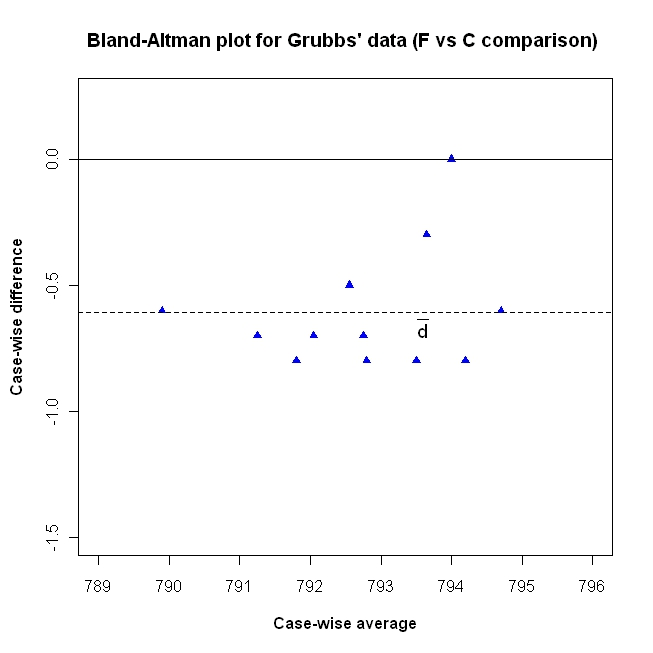
\includegraphics[width=120mm]{images/GrubbsBAplot-noLOA.jpeg}
			\caption{Bland-Altman plot For Fotobalk and Counter methods.}\label{GrubbsBA-noLOA}
		\end{center}
	\end{figure}
	
	
	
	In Figure 1.3 Bland-Altman plots for the `F vs C' and `F vs T'
	comparisons are shown, where `F vs T' refers to the comparison of
	the `Fotobalk' and `Terma' methods. Usage of the Bland-Altman plot
	can be demonstrate in the contrast between these comparisons.
	
	\begin{figure}[h!]
		\begin{center}
			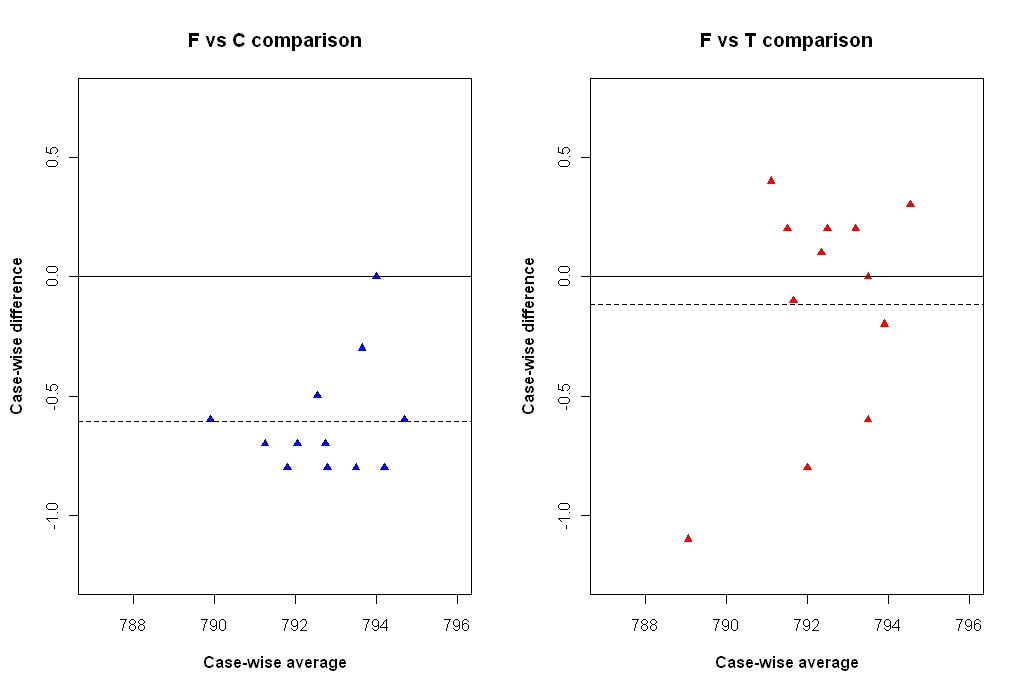
\includegraphics[height=90mm]{images/GrubbsDataTwoBAplots.jpeg}
			\caption{Bland-Altman plots for Grubbs' F vs C and F vs T comparisons.}\label{GrubbsDataTwoBAplots}
		\end{center}
	\end{figure}
	
	By inspection, there exists a larger inter-method bias in the `F
	vs C' comparison than in the `F vs T' comparison. Conversely there
	appears to be less precision in`F vs T' comparison, as indicated
	by the greater dispersion of co-variates.
	
	Figures 1.4, 1.5 and 1.6 are three prototype Bland-Altman plots
	derived from simulated data, each for the purpose of demonstrating
	how the plot would inform an analyst of features that would
	adversely affect use of the recommended methodology.
	
	Figure 1.4 demonstrates how the Bland-Altman plot would indicate
	increasing variance of differences over the measurement range.
	Fitted regression lines, for both the upper and lower half of the
	plot, has been added to indicate the trend. Figure 1.5 is an
	example of cases where the inter-method bias changes over the
	measurement range. This is known as proportional bias. In both
	Figures 1.4 and 1.5, the assumptions necessary for further
	analysis using the limits of agreement are violated.
	
	Application of regression techniques to the Bland-Altman plot, and
	subsequent formal testing for the constant variability of
	differences is informative. The data set may be divided into two
	subsets, containing the observations wherein the difference values
	are less than and greater than the inter-method bias respectively.
	For both of these fits, hypothesis tests for the respective slopes
	can be performed. While both tests can be considered separately,
	multiple comparison procedures, such as the Benjamini-Hochberg
	\citep{BH} test, should be also be used.
	
	\begin{figure}[h!]
		\begin{center}
			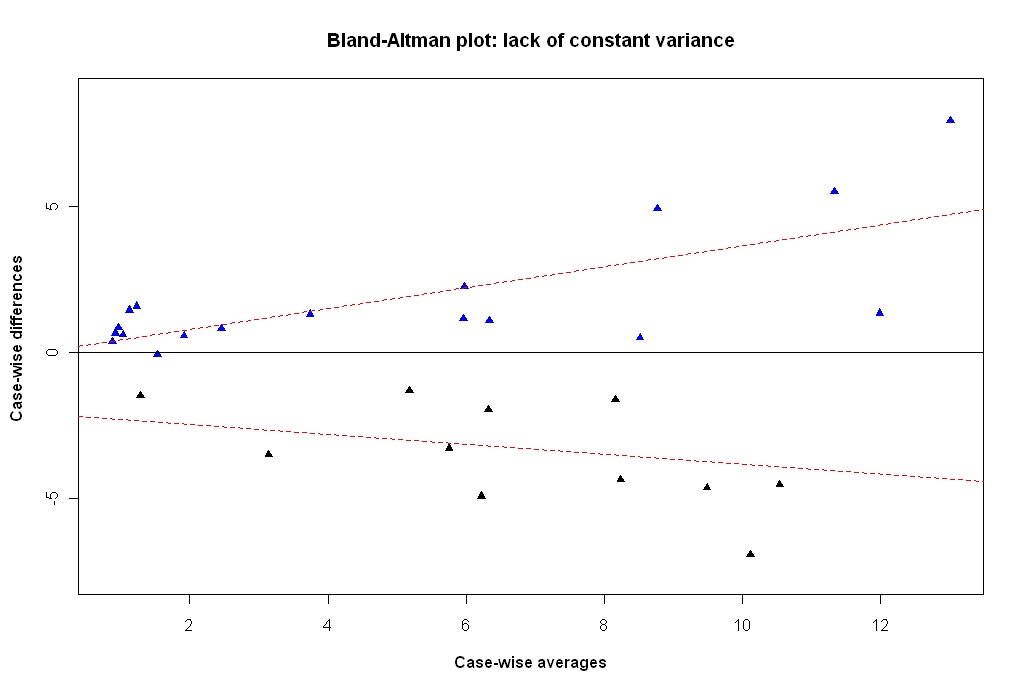
\includegraphics[height=90mm]{images/BAFanEffect.jpeg}
			\caption{Bland-Altman plot demonstrating the increase of variance over the range.}\label{BAFanEffect}
		\end{center}
	\end{figure}
	
	\begin{figure}[h!]
		\begin{center}
			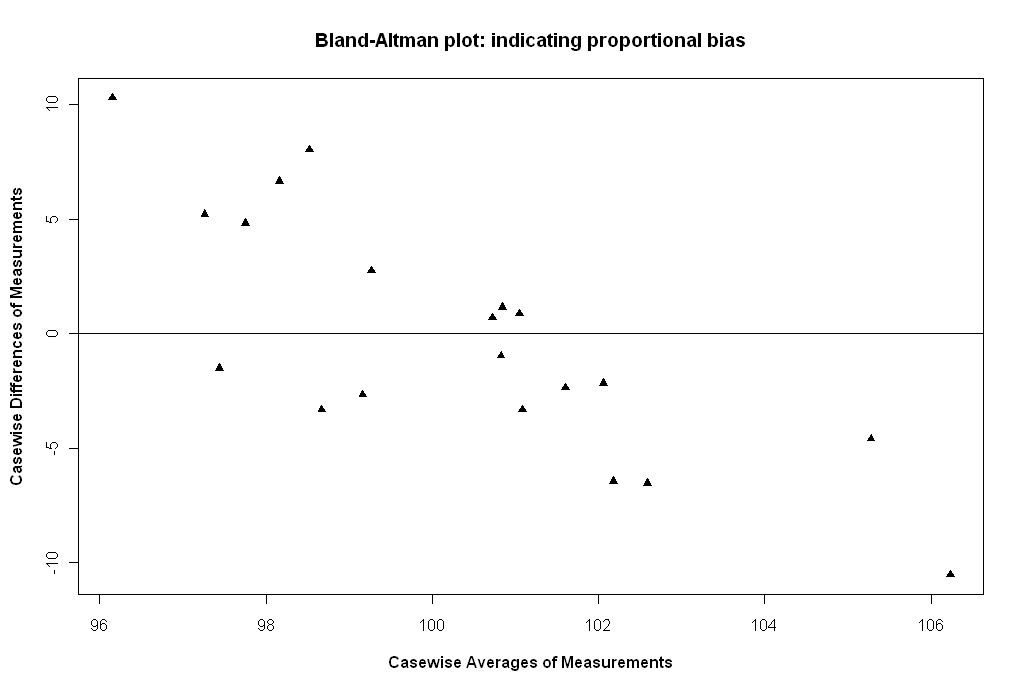
\includegraphics[height=90mm]{images/PropBias.jpeg}
			\caption{Bland-Altman plot indicating the presence of proportional bias.}\label{PropBias}
		\end{center}
	\end{figure}
	
	\begin{figure}[h!]
		\begin{center}
			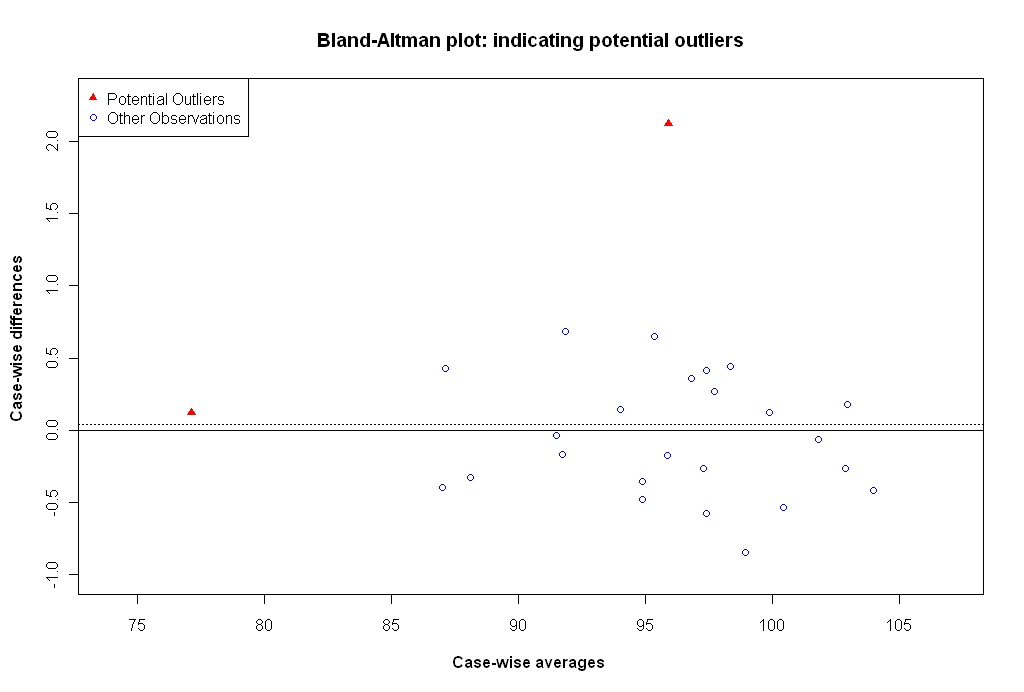
\includegraphics[width=125mm]{images/BAOutliers.jpeg}
			\caption{Bland-Altman plot indicating the presence of potential outliers.}\label{Outliers}
		\end{center}
	\end{figure}
	
	
	% outliers
	
	
	The Bland-Altman plot also can be used to identify outliers. An
	outlier is an observation that is conspicuously different from the
	rest of the data that it arouses suspicion that it occurs due to a
	mechanism, or conditions, different to that of the rest of the
	observations. Classification of outliers can be determined with
	numerous established approaches, such as the Grubb's test, but
	always classification must be informed by the logic of the data's
	formulation. Figure 1.6 is a Bland-Altman plot with two potential
	outliers.
	
	
	\citet*{BA99} do not recommend excluding outliers from analyses,
	but remark that recalculation of the inter-method bias estimate,
	and further calculations based upon that estimate, are useful for
	assessing the influence of outliers. The authors remark that `we
	usually find that this method of analysis is not too sensitive to
	one or two large outlying differences'.
	
	
	%\citet{Grubbs} defined an outlier as a co-variate that appears to
	%deviate markedly from other members of the sample in which it
	%occurs.
	
	In classifying whether a observation from a univariate data set is
	an outlier, Grubbs' outlier test is widely used. In assessing
	whether a co-variate in a Bland-Altman plot is an outlier, this
	test is useful when applied to the difference values treated as a
	univariate data set. For Grubbs' data, this outlier test is
	carried out on the differences, yielding the following results.
	
	The null and alternative hypotheses is the absence and presence of
	at least one outlier respectively. Grubbs' outlier test statistic
	$G$ is the largest absolute deviation from the sample mean divided
	by the standard deviation of the differences. For the `F vs C'
	comparison, $G = 3.6403$. The critical value is calculated using
	Student's $t$ distribution and the sample size,
	\begin{equation}
	U = \frac{n-1}{\sqrt{n}} \sqrt{\frac{t_{\alpha/(2n),n-2}^2}{n - 2
			+ t_{\alpha/(2n),n-2}^2}}.
	\end{equation}
	
	For this test $U = 0.7501$. The conclusion of this test is that
	the fourth observation in the `F vs C' comparison is an outlier,
	with $p-value = 0.002799$.
	
	As a complement to the Bland-Altman plot, \citet{Bartko} proposes
	the use of a bivariate confidence ellipse, constructed for a
	predetermined level.
	
	The minor axis relates to the between subject variability, whereas
	the major axis relates to the error mean square, with the ellipse
	depicting the size of both relative to each
	other.\citet{AltmanEllipse} provides the relevant calculations for
	the ellipse. Bartko states that the ellipse can, inter alia, be
	used to detect the presence of outliers (furthermore
	\citet{Bartko} proposes formal testing procedures, that shall be
	discussed in due course). Inspection of Figure 1.7 shows that the
	fourth observation is outside the bounds of the ellipse,
	concurring with the conclusion that it is an outlier.
	
	
	\begin{figure}[h!]
		% Requires \usepackage{graphicx}
		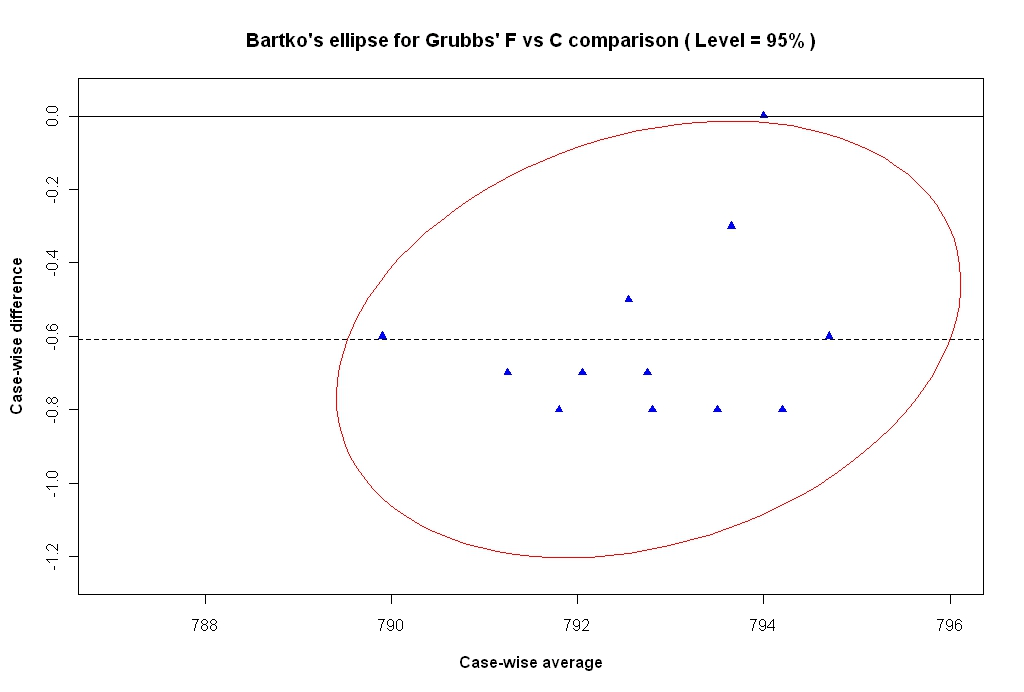
\includegraphics[width=130mm]{images/GrubbsBartko.jpeg}
		\caption{Bartko's Ellipse For Grubbs' Data.}\label{GrubbsBartko}
	\end{figure}
	
	The limitations of using bivariate approaches to outlier detection
	in the Bland-Altman plot can demonstrated using Bartko's ellipse.
	A co-variate is added to the `F vs C' comparison that has a
	difference value equal to the inter-method bias, and an average
	value that markedly deviates from the rest of the average values
	in the comparison, i.e. 786. Table 1.8 depicts a $95\%$ confidence
	ellipse for this enhanced data set. By inspection of the
	confidence interval, a conclusion would be reached that this extra
	co-variate is an outlier, in spite of the fact that this
	observation is consistent with the intended conclusion of the
	Bland-Altman plot.
	
	\begin{figure}[h!]
		% Requires \usepackage{graphicx}
		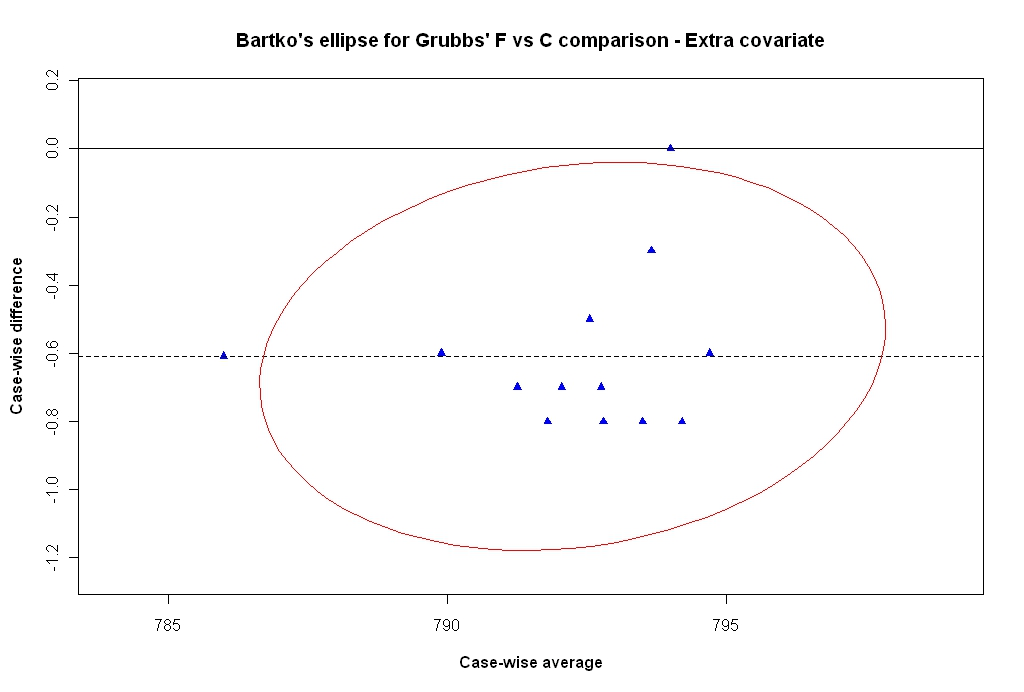
\includegraphics[width=130mm]{images/GrubbsBartko2.jpeg}
		\caption{Bartko's Ellipse For Grubbs' Data, with an extra covariate.}\label{GrubbsBartko2}
	\end{figure}
	
	In the Bland-Altman plot, the horizontal displacement of any
	observation is supported by two independent measurements. Any
	observation should not be considered an outlier on the basis of a
	noticeable horizontal displacement from the main cluster, as in
	the case with the extra co-variate. Conversely, the fourth
	observation, from the original data set, should be considered an
	outlier, as it has a noticeable vertical displacement from the
	rest of the observations.
	
	Bartko's ellipse provides a visual aid to determining the
	relationship between variances. If $\mbox{var}(a_{i})$ is greater
	than $\mbox{var}(d_{i})$, the orientation of the ellipse is
	horizontal. Conversely if $\mbox{var}(a_{i})$ is less than
	$\mbox{var}(d_{i})$, the orientation of the ellipse is vertical.
	\newpage
	
	
	
	%\begin{figure}[h!]
	%\begin{center}
	%  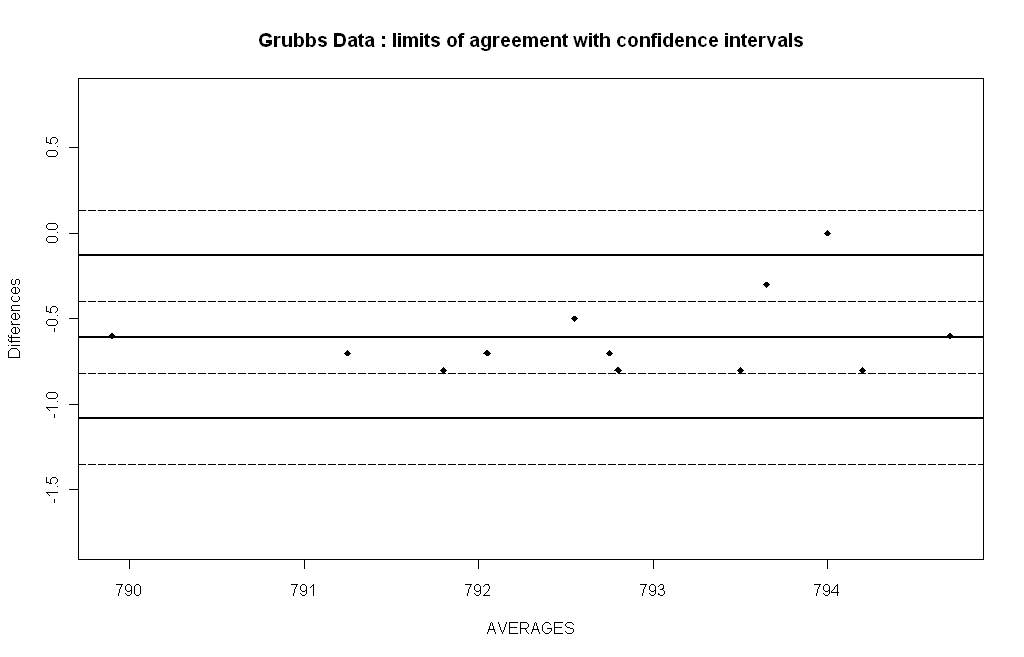
\includegraphics[width=125mm]{images/GrubbsLOAwCIs.jpeg}
	%  \caption{Limits of agreement with confidence intervals}\label{LOAwCIs}
	%\end{center}
	%\end{figure}
	
	%================================================================ %
	% USED
	\subsection{Variations of the Bland-Altman Plot} Referring to the
	assumption that bias and variability are constant across the range
	of measurements, \citet{BA99} address the case where there is an
	increase in variability as the magnitude increases. They remark
	that it is possible to ignore the issue altogether, but the limits
	of agreement would wider apart than necessary when just lower
	magnitude measurements are considered. Conversely the limits would
	be too narrow should only higher magnitude measurements be used.
	To address the issue, they propose the logarithmic transformation
	of the data. The plot is then formulated as the difference of
	paired log values against their mean. Bland and Altman acknowledge
	that this is not easy to interpret, and may not be suitable in
	all cases.
	
	\citet{BA99} offers two variations of the Bland-Altman plot that
	are intended to overcome potential problems that the conventional
	plot would inappropriate for. The first variation is a plot of
	casewise differences as percentage of averages, and is appropriate
	when there is an increase in variability of the differences as the
	magnitude increases. The second variation is a plot of casewise
	ratios as percentage of averages. This will remove the need for
	log transformation. This approach is useful when there is an
	increase in variability of the differences as the magnitude of the
	measurement increases. \citet{Eksborg} proposed such a ratio plot,
	independently of Bland and Altman. \citet{Dewitte} commented on
	the reception of this article by saying `Strange to say,this
	report has been overlooked'.
	%USED
	%=============================================== %
	
	
	
	
	\subsection{Regression-based Limits of Agreement} Assuming that
	there will be no curvature in the scatter-plot, the methodology
	regresses the difference of methods ($d$) on the average of those
	methods ($a$) with a simple intercept slope model; $\hat{d} =
	b_{0}+ b_{1}a.$ Should the slope $b_{1}$ be found to be
	negligible, $\hat{d}$ takes the value $\bar{d}$.
	
	The next step to take in calculating the limits is also a
	regression, this time of the residuals as a function of the scale
	of the measurements, expressed by the averages $a_{i}$;
	$ \hat{R} = c_{0}+ c_{1}a_{i}$
	
	With reference to absolute values following a half-normal
	distribution with mean $\sigma\sqrt{\frac{2}{\pi}}$, \citet{BA99} formulate the regression based limits of agreement as
	follows
	\begin{equation}
	\hat{d} \pm 1.96\sqrt{\frac{\pi}{2}}\hat{R} = \hat{d} \pm 2.46\hat{R}
	\end{equation}
	
	\subsection{Replicate Measurements}
	
	Thus far, the formulation for comparison of two measurement
	methods is one where one measurement by each method is taken on
	each subject. Should there be two or more measurements by each
	methods, these measurement are known as `replicate measurements'.
	\citet{BXC2008} recommends the use of replicate measurements, but
	acknowledges that  additional computational complexity.
	
	\citet*{BA86} address this problem by offering two different
	approaches. The premise of the first approach is that replicate
	measurements can be treated as independent measurements. The
	second approach is based upon using the mean of the each group of
	replicates as a representative value of that group. Using either
	of these approaches will allow an analyst to estimate the inter
	method bias.
	
	%\subsubsection{Mean of Replicates Limits of Agreement}
	
	However, because of the removal of the effects of the replicate
	measurements error, this would cause the estimation of the
	standard deviation of the differences to be unduly small.
	\citet*{BA86} propose a correction for this.
	
	\citet{BXC2008} takes issue with the limits of agreement based on
	mean values, in that they can only be interpreted as prediction
	limits for difference between means of repeated measurements by
	both methods, as opposed to the difference of all measurements.
	Incorrect conclusions would be caused by such a misinterpretation.
	\citet{BXC2008} demonstrates how the limits of agreement
	calculated using the mean of replicates are `much too narrow as
	prediction limits for differences between future single
	measurements'. This paper also comments that, while treating the
	replicate measurements as independent will cause a downward bias
	on the limits of agreement calculation, this method is preferable
	to the `mean of replicates' approach.
	
	The approach proposed by \citet{BA83} is a formal test on the
	Pearson correlation coefficient of case-wise differences and means
	($\rho_{ad}$). According to the authors, this test is equivalent
	to the `Pitman Morgan Test'. For the Grubbs data, the correlation
	coefficient estimate ($r_{ad}$) is 0.2625, with a 95\% confidence
	interval of (-0.366, 0.726) estimated by Fishers `r to z'
	transformation \citep*{Cohen}. The null hypothesis ($\rho_{ad}$
	=0)would fail to be rejected. Consequently the null hypothesis of
	equal variances of each method would also fail to be rejected.
	There has no been no further mention of this particular test in
	\citet{BA86}, although \citet{BA99} refers to Spearman's rank
	correlation coefficient. \citet{BA99} comments `we do not see a
	place for methods of analysis based on hypothesis testing'.
	\citet{BA99} also states that consider structural equation models
	to be inappropriate.
	
	\citet{DunnSEME} highlights an important issue regarding using
	models such as these, the identifiability problem. This comes as a
	result of there being too many parameters to be estimated.
	Therefore assumptions about some parameters, or estimators used,
	must be made so that others can be estimated. For example $\alpha$
	may take the value of the inter-method bias estimate from
	Bland-Altman methodology. Another assumption is that the precision
	ratio $\lambda=\frac{\sigma^{2}_{\epsilon}}{\sigma^{2}_{\delta}}$
	may be known.
	
	
	\citet{DunnSEME} considers methodologies based on two methods with single measurements on each subject as inadequate for a serious study
	on the measurement characteristics of the methods. This is because there would not be enough data to allow for a meaningful analysis.
	There is, however, a contrary argument that is very difficult to get replicate
	observations when the measurement method requires invasive medical procedure.
	
	\citet{DunnSEME} recommends the following approach for analyzing
	method comparison data. Firstly he recommends conventional
	Bland-Altman methodology; plotting the scatterplot and the
	Bland-Altman plot, complemented by estimate for the limits of
	agreement and the correlation coefficient between the difference
	and the mean. Additionally boxplots may be useful in considering
	the marginal distributions of the observations. The second step is
	the calculations of summary statistics; the means and variances of
	each set of measurements, and the covariances.
	%Should covariance values be greater than the either of the two variances,
	
	When both methods measure in the same scale (i.e. $\beta = 1$),
	\citet{DunnSEME} recommends the use of Grubbs estimators to
	estimate error variances, and to test for their equality. A test
	of whether the intercept $\alpha$ may be also be appropriate.
	
	
	
	%This application of the
	%Grubbs method presumes the existence of this condition, and necessitates
	%replication of observations by means external to and independent of the first
	%means. The Grubbs estimators method is based on the laws of propagation of
	%error. By making three independent simultaneous measurements on the same
	%physical material, it is possible by appropriate mathematical manipulation of
	%the sums and differences of the associated variances to obtain a valid
	%estimate of the precision of the primary means. Application of the Grubbs
	%estimators procedure to estimation of the precision of an apparatus uses
	%the results of a physical test conducted in such a way as to obtain a series
	%of sets of three independent observations.
	
	
	
	%%%%%%%%%%%%%%%%%%%%%%%%%%%%%%%%%%%%%%%%%%%%%%%%%%%%%%%%%%%%%%%%%%%%%%%%%%%%%%%%%%%%%%%%%%%%%%%%%%%%%%%%
	
	%%%%%%%%%%%%%%%%%%%%%%%%%%%%%%%%%%%%%%%%%%%%%%%%%%%%%%%%%%%%%%%%%%%%%%%%%%%%%%%%%%%%%%%%%%%%%%%%%%%%%%%%
	\newpage

\section{MCS Data Sets}
\begin{enumerate}
	\item Blood Data
	\item Cardiac Data
	\item Nadler Hurley 
\end{enumerate}

%%%%%%%%%%%%%
%1 Method Comparison Studies            %%%%%%%%%%%%%%%%%%%%%%%%%%%%%%%%%
%%%%%%%%%%%%%%%%%%%%%%%%%%%%%%%%%%%%%%%%%%%%%%%%%%%%%%%%%%%%%%%%%%%%%%%%%
\begin{itemize}		
	%-------------------------------------------------%
	% Chapter 1
	
	\item	Introduction to Method Comparison Studies	
	\begin{itemize}	
		\item	Accuracy and Precision
		\item	Repeatability (Bland Altman 1999)
		\item	Barnharts Paper
		\item	
	\end{itemize}	
	
	%-------------------------------------------------%
	% Chapter 2
	
	\item	Bland and Altman Plot	
	\begin{itemize}	
		\item	Bland and Altman 1983 and 86
		\item	Limits of Agreement
		\item	
		\item	
	\end{itemize}

	
\end{itemize}		

%====================================================================%

\section{Introduction}

Outliers and detection of influent observations is an important step in the analysis of a data set. There are several ways of evaluating the influence of perturbations in the data set and in the model given the parameter estimates. 

\subsection{Overview of R implementations}
Further to previous material, an appraisal of the current state of development (or lack thereof) for current implemenations for LME models, particularly for \texttt{nlme} and \texttt{lme4} fitted models.

Crucially, a review of internet resources indicates that almost all of the progress in this regard has been done for \texttt{lme4} fitted models, specifically the \textit{Influence.ME} \texttt{R} package. (Nieuwenhuis et al 2014)
Conversely there is very little for \texttt{nlme} models. One would immediately look at the current development workflow for both packages.

%======================%
% Douglas Bates

As an aside, Douglas Bates was arguably the most prominent \texttt{R} developer working in the LME area. 
However Bates has now prioritised the development of LME models in another computing environment , i.e Julia. 
% The current version of this is XXXX

%======================%
% nlme

With regards to \texttt{nlme}, the package is now maintained by the \texttt{R} core development team. The most recent major text is by Galecki \& Burzykowski, who have published \textit{ Linear Mixed Effects Models using \texttt{R}. }
Also, the accompanying \texttt{R} package, nlmeU package is under current development, with a version being released $0.70-3$.


%======================%
% lme4 and influence.ME

The \textbf{lme4} pacakge is used to fit linear and generalized linear mixed-effects models in the R environment.
The \textbf{lme4} package is also under active development, under the leadership of Ben Bolker (McMaster Uni., Canada).


%=====================%
\subsection*{Important Consideration for MCS}

The key issue is that \texttt{nlme} allows for the particular specification of Roy's Model, speciifically direct specification of the VC matrices for within subject and between subject residuals.
The \texttt{lme4} package does not allow for Roy's Model, for reasons that will identified shortly.
To advance the ideas that eminate from Roys' paper, one is required to use the \texttt{nlme} context. However, to take advantage of the infrastructure already provided for \texttt{lme4} models, one may change the research question away from that of Roy's paper. 
To this end, an exploration of what textbf{influence.ME} can accomplished is merited.




%--------------------------------------------------------------%
\newpage
\section{Computation and Notation } %2.3
with $\boldsymbol{V}$ unknown, a standard practice for estimating $\boldsymbol{X \beta}$ is the estime the variance components $\sigma^2_j$,
compute an estimate for $\boldsymbol{V}$ and then compute the projector matrix $A$, $\boldsymbol{X \hat{\beta}}  = \boldsymbol{AY}$.


Zewotir remarks that $\boldsymbol{D}$ is a block diagonal with the $i-$th block being $u \boldsymbol{I}$

\section{ Liao Shaio}

Lai et Shiao is interesting in that it extends the usual method comparison study question. It correctly identifies LME models as a methodoloy that can used to make such questions tractable.
The Data Set used in their examples is unavailable for independent use. Therefore, for the sake of consistency, a data set will be simulated based on the Blood Data that will allow for extra variables.



%============================================================================%

% - http://journal.r-project.org/archive/2012-2/RJournal_2012-2_Nieuwenhuis~et~al.pdf

% - http://www.rensenieuwenhuis.nl/tag/lme4/

% - http://lme4.r-forge.r-project.org/lMMwR/lrgprt.pdf

%============================================================================%

A Study of the Bland-Altman Plot and its Associated Methodology

Joseph G. Voelkel Bruce E. Siskowski 

% - https://www.rit.edu/kgcoe/cqas/sites/rit.edu.kgcoe.cqas/files/docs/TR%202005-3.pdf

%============================================================================%

% - http://sprouts.aisnet.org/785/1/TAMReview.pdf
% - http://organizacija.fov.uni-mb.si/index.php/organizacija/article/viewFile/557/999
\section{Limits of agreement for Carstensen's data}


\citet{bxc2008} describes the calculation of the limits of agreement (with the inter-method bias implicit) for both data sets, based on his formulation;

\[\hat{\alpha}_1 - \hat{\alpha}_2 \pm 2\sqrt{2\hat{\tau}^2 +\hat{\sigma}_1^2 +\hat{\sigma}_2^2 }.\]

For the `Fat' data set, the inter-method bias is shown to be $0.045$. The limits of agreement are $(-0.23 , 0.32)$

Carstensen demonstrates the use of the interaction term when computing the limits of agreement for the `Oximetry' data set. When the interaction term is omitted, the limits of agreement are $(-9.97, 14.81)$. Carstensen advises the inclusion of the interaction term for linked replicates, and hence the limits of agreement are recomputed as $(-12.18,17.12)$.






%-----------------------------------------------------------------------------------------------------%
\newpage
\section{Hamlett and Lam}
The methodology proposed by \citet{Roy2009} is largely based on \citet{hamlett}, which in turn follows on from \citet{lam}.

%Lam 99
%In many cases, repeated observation are collected from each subject in sequence  and/or longitudinally.

%Hamlett
%Hamlett re-analyses the data of lam et al to generalize their model to cover other settings not covered by the Lam %method.






The desired outcome of this research is to

\begin{itemize}
	\item Formulate a methodology that represents Best practice in Method Comparison Studies. Indeed the methodology is envsiaged to advance what is considered best practice, inter alia, by making diagnostics procedures a standard part of MCS. 
	
	\item Provide for ease of use such that non-statisticians can master and implement the method, with a level of training that one would expect 
	as part of a Professional CPD programe.
	
\end{itemize}

Apropos of the matter of ease-of-use, certain assumptions must be made.


The user has a reasonable amount of computer literacy.
The user would have a reasonable understanding of statistics, consistent with an undergraduate statistics module. 
That is to say, that the user is acquainted with the idea of $p-$values.

Easy to follow set of instructions to properly implement the method.

%==============================================================================%

Linear Mixed Effects Models can be implemented by using one of the following R packages.
lme4
nlme

The first package to be introducted was nlme, developled by Jose Pinheiro and Douglas Bates ( Authors of the the companion textbook, NAME)

As this package has been under ongoing development for quite a long time, it is now allows for a lot of complex LME implementations. 
Furthermore, nlme is one of the base R packages.  That is to say, when one downloads and installs R, nlme is automatically installed also, and can be called immediately.

Having said that, the authors have pointed to several limitations of the overall methodology thrugh R.
The original developers have both left the project, but other statisticians have taken over the development, and indeed a new version of nlme was released.

LME4 is a more recent package. at a glance, the syntax is easier, but the development is less advanced. There are several functionalities that can not be implemented with lme4 yet. 
As an example - CHAP5 in PB - has no equivalent in LME4. Indeed no textbook exists to co-incide with LME4.

The main author, Douglas Bates, has turned his attention to development of LME models in the Julia programming language.

The nlmeU package is described by its authors as an extesntion of the nlme package, and indeed provides for additionally functionality. The package is also useful as it serves as a companion piece to the 
book by Galecki and Burzwhatski.

The nlme package also allows for the specification of GLS models.

%-----------------------------------------------------------------------------%
\subsection*{Objects and Classes}

The main nlme object is an \texttt{nlme} model.

The main lme4 object is called an \texttt{lmer} model

The lattice package is used for graphical methods.

%=============================================================================%

Model Diagnostics with \texttt{nlme}





\subsection{Inappropriate Techniques for MCS}


\subsection{Links and Papers}
\begin{verbatim}

Westgard Statistics  - http://www.westgard.com/lesson23.htm
\end{verbatim}





%==============================================================================%
\subsection*{Measurement Systems Analysis}The topic of measurement sensitivity anaylysis (MSA, also known as Gauge R\&R) is prevalent in industrial statistics (i.e Six Sigma).

There is extensive literature that covers the area. For the sake of brevity, we will use Cano et al.

For sake of clarity, Cano's definitions of repeatability and reproducibility are listed, with added emphasis.

Reproducibility is rarely, if ever, discussed in the domain of Method Comparison Studies. This may be due to the fact that prevalent methodologies can be used for the problem.However
the methodologies proposed by this research can easily be extended.




	\chapter{Introduction}
	
	
	\section{Bland-Altman Plots}
	The issue of whether two measurement methods comparable to the
	extent that they can be used interchangeably with sufficient
	accuracy is encountered frequently in scientific research.
	Historically comparison of two methods of measurement was carried
	out by use of paired sample t-test, correlation coefficients or
	simple linear regression. Statisticians Martin Bland and Douglas
	Altman recognized the inadequacies of these analyses and
	articulated quite thoroughly the basis on which of which they are
	unsuitable for comparing two methods of measurement \citep*{BA83}.
	Furthermore they proposed their simple methodology specifically
	constructed for method comparison studies. They acknowledge the
	opportunity to apply other valid, but complex, methodologies, but
	argue that a simple approach is preferable, especially when the
	results must be `explained to non-statisticians'.
	
	Notwithstanding previous remarks about regression, the first step
	recommended, which the authors argue should be mandatory, is
	construction of a simple scatter plot of the data. The line of
	equality should also be shown, as it is necessary to give the
	correct interpretation of how both methods compare. A scatter plot
	of the Grubbs data is shown in Figure 1.1. Visual inspection confirms the previous conclusion that there is an
	inter-method bias present, i.e. Fotobalk device has a tendency to
	record a lower velocity.
	
	\begin{figure}[h!]
		\begin{center}
			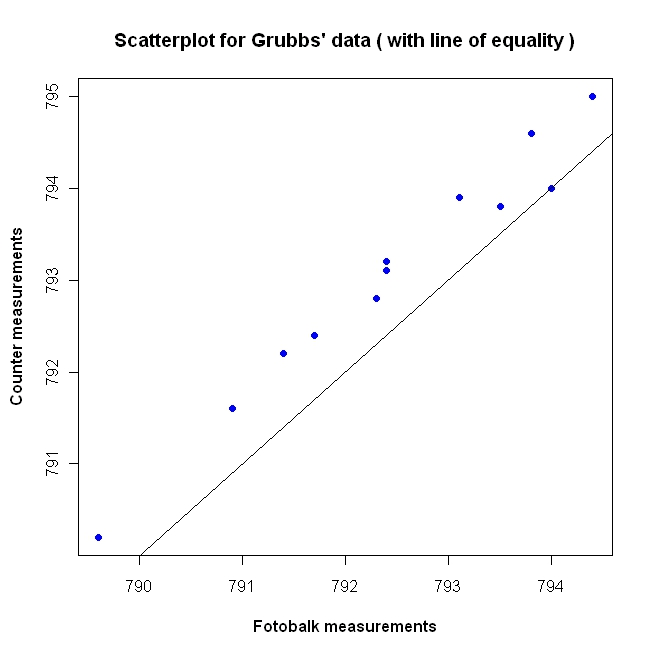
\includegraphics[width=130mm]{images/GrubbsScatter.jpeg}
			\caption{Scatter plot For Fotobalk and Counter Methods.}\label{GrubbsScatter}
		\end{center}
	\end{figure}
	
	In light of shortcomings associated with scatterplots,
	\citet*{BA83} recommend a further analysis of the data. Firstly
	case-wise differences of measurements of two methods $d_{i} =
	y_{1i}-y_{2i} \mbox{ for }i=1,2,..n$ on the same subject should be
	calculated, and then the average of those measurements ($a_{i} =
	(y_{1i} + y_{2i})/2 \mbox{ for }i=1,2,..n$). These differences and
	averages are then plotted. This methodology, now commonly known as
	the `Bland-Altman Plot', has proved very successful.
	\citet*{BA86}, which further develops the methodology, was found
	to be the sixth most cited paper of all time by the
	\citet{BAcite}. \cite{Dewitte} also commented on the rate at which
	prevalence of the Bland-Altman plot has developed in scientific
	literature. The Bland-Altman Plot has since become expected, and
	often obligatory, approach for presenting method comparison
	studies in many scientific journals \citep{hollis}. Furthermore
	\citet{BritHypSoc} recommend its use in papers pertaining to
	method comparison studies for the journal of the British
	Hypertension Society.
	
	The magnitude of the inter-method bias between the two methods is
	simply the average of the differences $\bar{d}$. The variances
	around this bias is estimated by the standard deviation of the
	differences $S(d)$. This inter-method bias is represented with a
	line on the Bland-Altman plot. These estimates are only meaningful
	if there is uniform inter-bias and variability throughout the
	range of measurements, which can be checked by visual inspection
	of the plot. In the case of Grubbs data the inter-method bias is
	$-0.61$ metres per second, and is indicated by the dashed line on
	Figure 1.2. By inspection of the plot, it is also possible to
	compare the precision of each method. Noticeably the differences
	tend to increase as the averages increase.
	
	
	\begin{table}[h!]
		\renewcommand\arraystretch{0.7}%
		\begin{center}
			\begin{tabular}{|c||c|c||c|c|}
				\hline
				Round & Fotobalk  & Counter  & Differences  & Averages  \\
				&  [F] & [C] & [F-C] &  [(F+C)/2] \\
				\hline
				1 & 793.8 & 794.6 & -0.8 & 794.2 \\
				2 & 793.1 & 793.9 & -0.8 & 793.5 \\
				3 & 792.4 & 793.2 & -0.8 & 792.8 \\
				4 & 794.0 & 794.0 & 0.0 & 794.0 \\
				5 & 791.4 & 792.2 & -0.8 & 791.8 \\
				6 & 792.4 & 793.1 & -0.7 & 792.8 \\
				7 & 791.7 & 792.4 & -0.7 & 792.0 \\
				8 & 792.3 & 792.8 & -0.5 & 792.5 \\
				9 & 789.6 & 790.2 & -0.6 & 789.9 \\
				10 & 794.4 & 795.0 & -0.6 & 794.7 \\
				11 & 790.9 & 791.6 & -0.7 & 791.2 \\
				12 & 793.5 & 793.8 & -0.3 & 793.6 \\
				\hline
			\end{tabular}
			\caption{Fotobalk and Counter methods: differences and averages.}
		\end{center}
	\end{table}
	
	\begin{table}[h!]
		\renewcommand\arraystretch{0.7}%
		\begin{center}
			\begin{tabular}{|c||c|c||c|c|}
				\hline
				Round & Fotobalk  & Terma  & Differences  & Averages  \\
				&  [F] & [T] & [F-T] &  [(F+T)/2] \\
				\hline
				1 & 793.80 & 793.20 & 0.60 & 793.50 \\
				2 & 793.10 & 793.30 & -0.20 & 793.20 \\
				3 & 792.40 & 792.60 & -0.20 & 792.50 \\
				4 & 794.00 & 793.80 & 0.20 & 793.90 \\
				5 & 791.40 & 791.60 & -0.20 & 791.50 \\
				6 & 792.40 & 791.60 & 0.80 & 792.00 \\
				7 & 791.70 & 791.60 & 0.10 & 791.65 \\
				8 & 792.30 & 792.40 & -0.10 & 792.35 \\
				9 & 789.60 & 788.50 & 1.10 & 789.05 \\
				10 & 794.40 & 794.70 & -0.30 & 794.55 \\
				11 & 790.90 & 791.30 & -0.40 & 791.10 \\
				12 & 793.50 & 793.50 & 0.00 & 793.50 \\
				
				\hline
			\end{tabular}
			\caption{Fotobalk and Terma methods: differences and averages.}
		\end{center}
	\end{table}
	
	\newpage
	
	
	\subsection{Using Bland-Altman Plots}
	Bland-Altman plots are a powerful graphical methodology for making
	a visual assessment of the data. \citet*{BA83} express the
	motivation for this plot thusly:
	\begin{quote}
		``From this type of plot it is much easier to assess the magnitude
		of disagreement (both error and bias), spot outliers, and see
		whether there is any trend, for example an increase in
		(difference) for high values. This way of plotting the data is a
		very powerful way of displaying the results of a method comparison
		study."
	\end{quote}
	
	The Bland-Altman plot is simply a scatterplot of the case-wise
	averages and differences of two methods of measurement. As the
	objective of the Bland-Altman plot is to advise on the agreement
	of two methods, it is the case-wise differences that are
	particularly. Later it will be shown that case-wise differences
	are the sole component of the next part of the methodology, the
	limits of agreement.
	
	For creating plots, the case wise-averages fulfil several
	functions, such as expressing the range over which the values were
	taken, and assessing whether the assumptions of constant variance
	holds. Case-wise averages also allow the case-wise differences to
	be presented on a two-dimensional plot, with better data
	visualization qualities than a one dimensional plot. \citet{BA86}
	cautions that it would be the difference against either
	measurement value instead of their average , as the difference
	relates to both value.
	
	The Bland-Altman plot for comparing the `Fotobalk' and `Counter'
	methods, which shall henceforth be referred to as the `F vs C'
	comparison,  is depicted in Figure 1.2, using data from Table 1.3.
	The presence and magnitude of the inter-method bias is indicated
	by the dashed line.
	
	\begin{figure}[h!]
		\begin{center}
			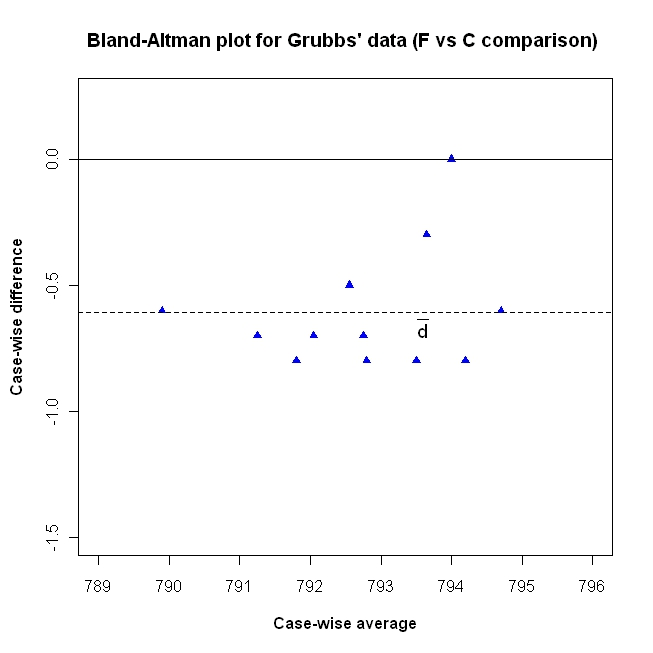
\includegraphics[width=120mm]{images/GrubbsBAplot-noLOA.jpeg}
			\caption{Bland-Altman plot For Fotobalk and Counter methods.}\label{GrubbsBA-noLOA}
		\end{center}
	\end{figure}
	
	
	
	In Figure 1.3 Bland-Altman plots for the `F vs C' and `F vs T'
	comparisons are shown, where `F vs T' refers to the comparison of
	the `Fotobalk' and `Terma' methods. Usage of the Bland-Altman plot
	can be demonstrate in the contrast between these comparisons.
	
	\begin{figure}[h!]
		\begin{center}
			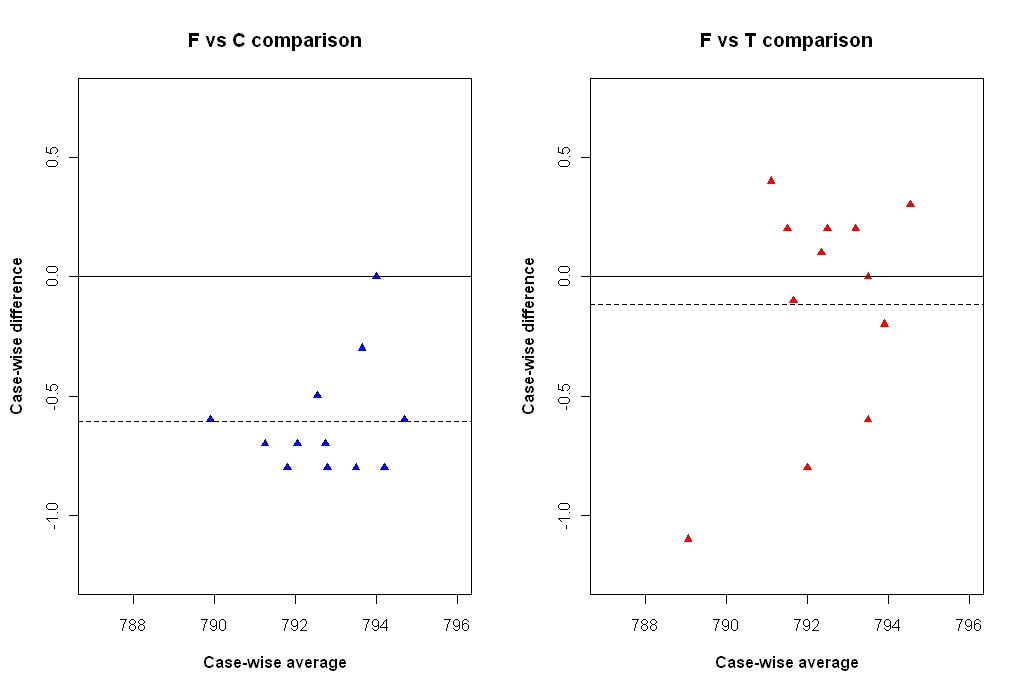
\includegraphics[height=90mm]{images/GrubbsDataTwoBAplots.jpeg}
			\caption{Bland-Altman plots for Grubbs' F vs C and F vs T comparisons.}\label{GrubbsDataTwoBAplots}
		\end{center}
	\end{figure}
	
	By inspection, there exists a larger inter-method bias in the `F
	vs C' comparison than in the `F vs T' comparison. Conversely there
	appears to be less precision in`F vs T' comparison, as indicated
	by the greater dispersion of co-variates.
	
	Figures 1.4, 1.5 and 1.6 are three prototype Bland-Altman plots
	derived from simulated data, each for the purpose of demonstrating
	how the plot would inform an analyst of features that would
	adversely affect use of the recommended methodology.
	
	Figure 1.4 demonstrates how the Bland-Altman plot would indicate
	increasing variance of differences over the measurement range.
	Fitted regression lines, for both the upper and lower half of the
	plot, has been added to indicate the trend. Figure 1.5 is an
	example of cases where the inter-method bias changes over the
	measurement range. This is known as proportional bias. In both
	Figures 1.4 and 1.5, the assumptions necessary for further
	analysis using the limits of agreement are violated.
	
	Application of regression techniques to the Bland-Altman plot, and
	subsequent formal testing for the constant variability of
	differences is informative. The data set may be divided into two
	subsets, containing the observations wherein the difference values
	are less than and greater than the inter-method bias respectively.
	For both of these fits, hypothesis tests for the respective slopes
	can be performed. While both tests can be considered separately,
	multiple comparison procedures, such as the Benjamini-Hochberg
	\citep{BH} test, should be also be used.
	
	\begin{figure}[h!]
		\begin{center}
			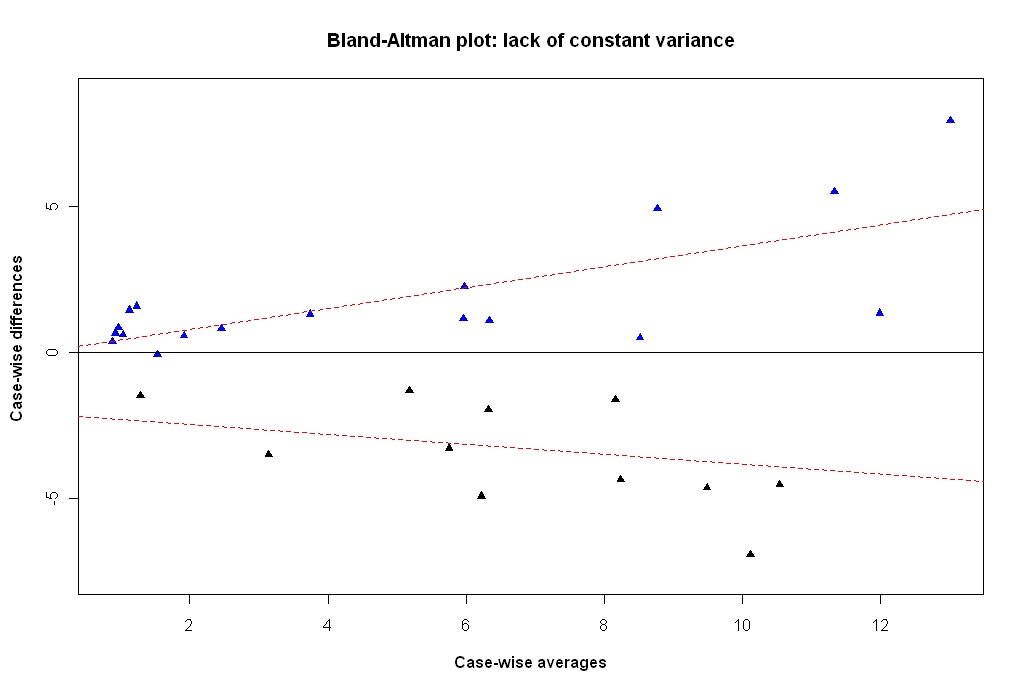
\includegraphics[height=90mm]{images/BAFanEffect.jpeg}
			\caption{Bland-Altman plot demonstrating the increase of variance over the range.}\label{BAFanEffect}
		\end{center}
	\end{figure}
	
	\begin{figure}[h!]
		\begin{center}
			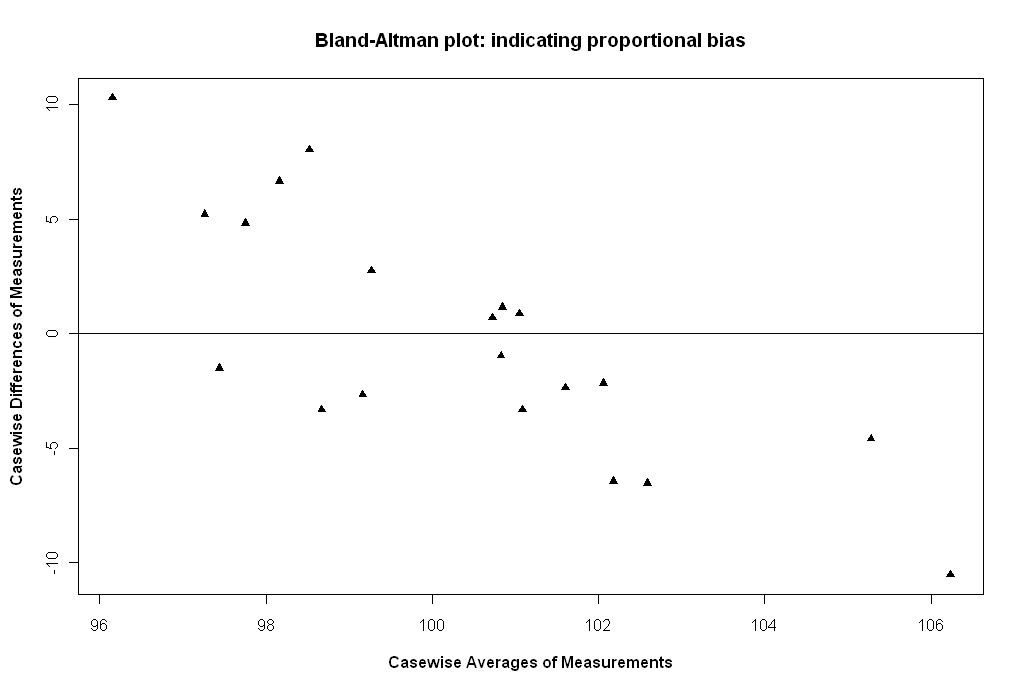
\includegraphics[height=90mm]{images/PropBias.jpeg}
			\caption{Bland-Altman plot indicating the presence of proportional bias.}\label{PropBias}
		\end{center}
	\end{figure}
	
	\begin{figure}[h!]
		\begin{center}
			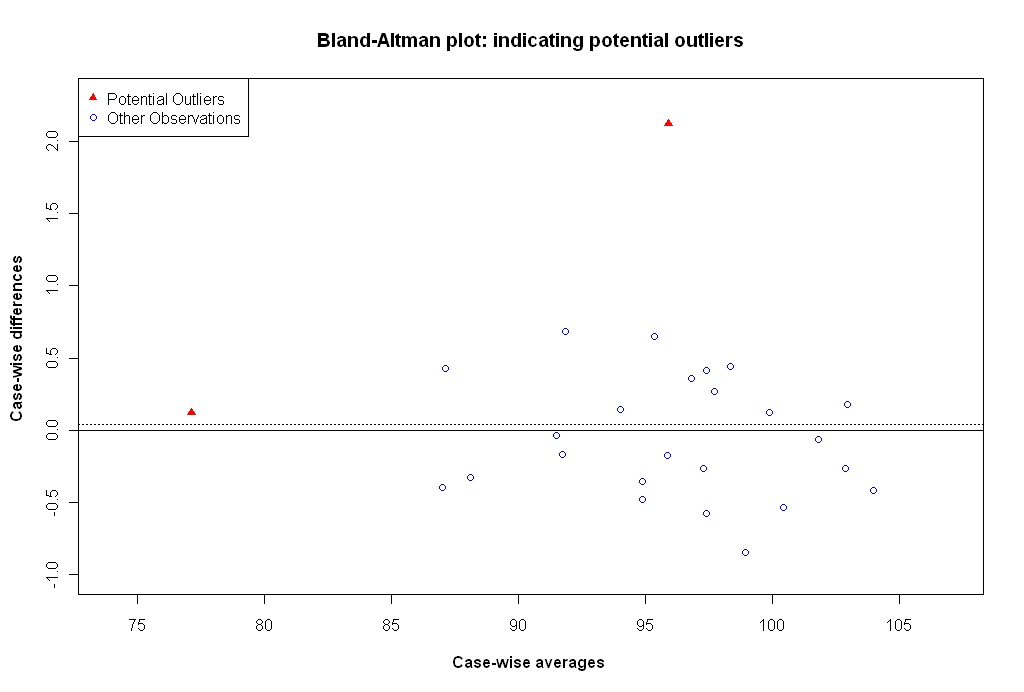
\includegraphics[width=125mm]{images/BAOutliers.jpeg}
			\caption{Bland-Altman plot indicating the presence of potential outliers.}\label{Outliers}
		\end{center}
	\end{figure}
	
	
	% outliers
	
	
	The Bland-Altman plot also can be used to identify outliers. An
	outlier is an observation that is conspicuously different from the
	rest of the data that it arouses suspicion that it occurs due to a
	mechanism, or conditions, different to that of the rest of the
	observations. Classification of outliers can be determined with
	numerous established approaches, such as the Grubb's test, but
	always classification must be informed by the logic of the data's
	formulation. Figure 1.6 is a Bland-Altman plot with two potential
	outliers.
	
	
	\citet*{BA99} do not recommend excluding outliers from analyses,
	but remark that recalculation of the inter-method bias estimate,
	and further calculations based upon that estimate, are useful for
	assessing the influence of outliers. The authors remark that `we
	usually find that this method of analysis is not too sensitive to
	one or two large outlying differences'.
	
	
	%\citet{Grubbs} defined an outlier as a co-variate that appears to
	%deviate markedly from other members of the sample in which it
	%occurs.
	
	In classifying whether a observation from a univariate data set is
	an outlier, Grubbs' outlier test is widely used. In assessing
	whether a co-variate in a Bland-Altman plot is an outlier, this
	test is useful when applied to the difference values treated as a
	univariate data set. For Grubbs' data, this outlier test is
	carried out on the differences, yielding the following results.
	
	The null and alternative hypotheses is the absence and presence of
	at least one outlier respectively. Grubbs' outlier test statistic
	$G$ is the largest absolute deviation from the sample mean divided
	by the standard deviation of the differences. For the `F vs C'
	comparison, $G = 3.6403$. The critical value is calculated using
	Student's $t$ distribution and the sample size,
	\begin{equation}
	U = \frac{n-1}{\sqrt{n}} \sqrt{\frac{t_{\alpha/(2n),n-2}^2}{n - 2
			+ t_{\alpha/(2n),n-2}^2}}.
	\end{equation}
	
	For this test $U = 0.7501$. The conclusion of this test is that
	the fourth observation in the `F vs C' comparison is an outlier,
	with $p-value = 0.002799$.
	
	As a complement to the Bland-Altman plot, \citet{Bartko} proposes
	the use of a bivariate confidence ellipse, constructed for a
	predetermined level.
	
	The minor axis relates to the between subject variability, whereas
	the major axis relates to the error mean square, with the ellipse
	depicting the size of both relative to each
	other.\citet{AltmanEllipse} provides the relevant calculations for
	the ellipse. Bartko states that the ellipse can, inter alia, be
	used to detect the presence of outliers (furthermore
	\citet{Bartko} proposes formal testing procedures, that shall be
	discussed in due course). Inspection of Figure 1.7 shows that the
	fourth observation is outside the bounds of the ellipse,
	concurring with the conclusion that it is an outlier.
	
	
	\begin{figure}[h!]
		% Requires \usepackage{graphicx}
		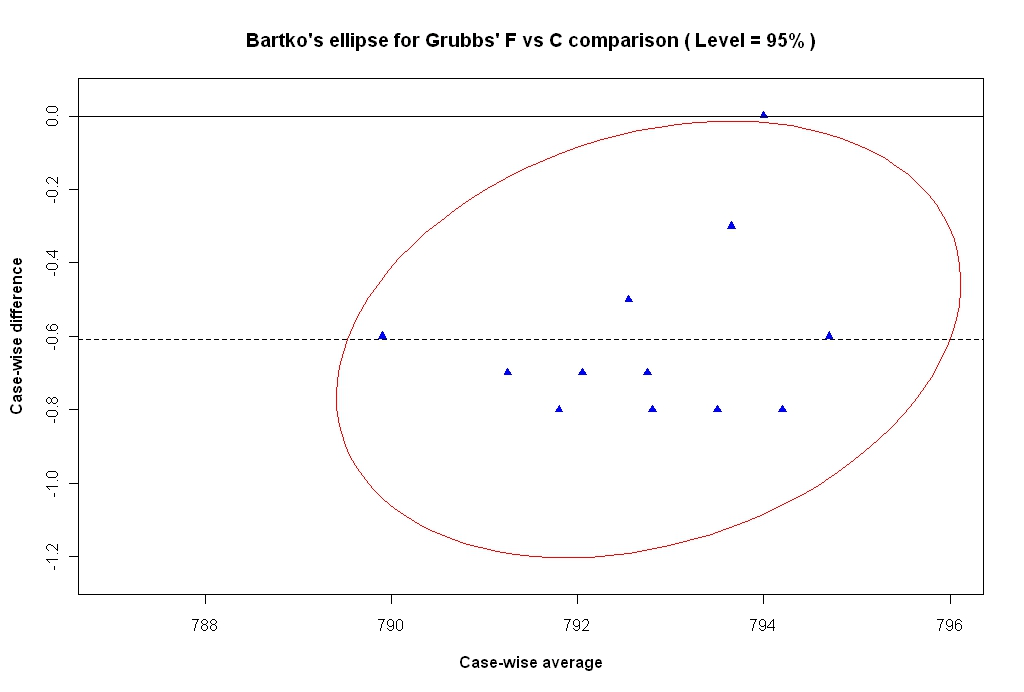
\includegraphics[width=130mm]{images/GrubbsBartko.jpeg}
		\caption{Bartko's Ellipse For Grubbs' Data.}\label{GrubbsBartko}
	\end{figure}
	
	The limitations of using bivariate approaches to outlier detection
	in the Bland-Altman plot can demonstrated using Bartko's ellipse.
	A co-variate is added to the `F vs C' comparison that has a
	difference value equal to the inter-method bias, and an average
	value that markedly deviates from the rest of the average values
	in the comparison, i.e. 786. Table 1.8 depicts a $95\%$ confidence
	ellipse for this enhanced data set. By inspection of the
	confidence interval, a conclusion would be reached that this extra
	co-variate is an outlier, in spite of the fact that this
	observation is consistent with the intended conclusion of the
	Bland-Altman plot.
	
	\begin{figure}[h!]
		% Requires \usepackage{graphicx}
		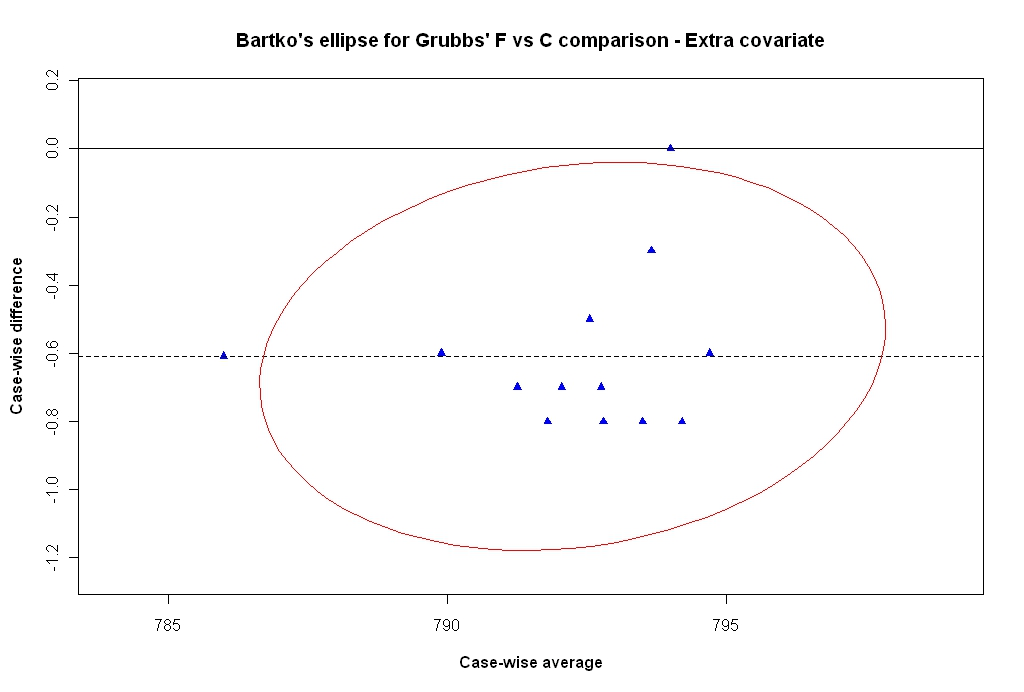
\includegraphics[width=130mm]{images/GrubbsBartko2.jpeg}
		\caption{Bartko's Ellipse For Grubbs' Data, with an extra covariate.}\label{GrubbsBartko2}
	\end{figure}
	
	In the Bland-Altman plot, the horizontal displacement of any
	observation is supported by two independent measurements. Any
	observation should not be considered an outlier on the basis of a
	noticeable horizontal displacement from the main cluster, as in
	the case with the extra co-variate. Conversely, the fourth
	observation, from the original data set, should be considered an
	outlier, as it has a noticeable vertical displacement from the
	rest of the observations.
	
	Bartko's ellipse provides a visual aid to determining the
	relationship between variances. If $\mbox{var}(a_{i})$ is greater
	than $\mbox{var}(d_{i})$, the orientation of the ellipse is
	horizontal. Conversely if $\mbox{var}(a_{i})$ is less than
	$\mbox{var}(d_{i})$, the orientation of the ellipse is vertical.
	\newpage
	
	
	
	%\begin{figure}[h!]
	%\begin{center}
	%  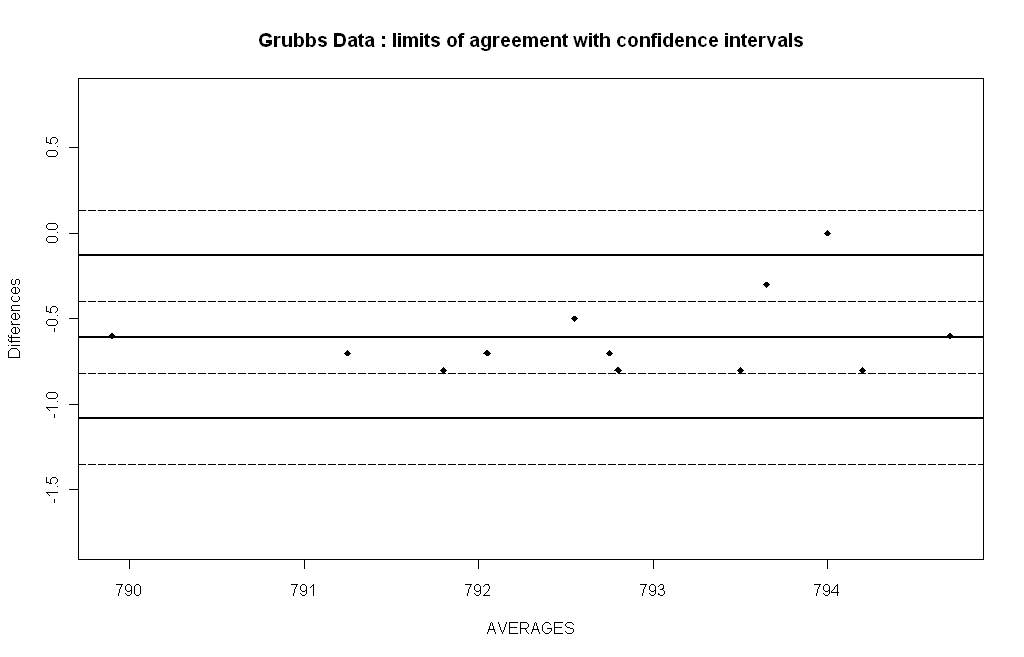
\includegraphics[width=125mm]{images/GrubbsLOAwCIs.jpeg}
	%  \caption{Limits of agreement with confidence intervals}\label{LOAwCIs}
	%\end{center}
	%\end{figure}
	
	\subsection{Variations of the Bland-Altman Plot} Referring to the
	assumption that bias and variability are constant across the range
	of measurements, \citet{BA99} address the case where there is an
	increase in variability as the magnitude increases. They remark
	that it is possible to ignore the issue altogether, but the limits
	of agreement would wider apart than necessary when just lower
	magnitude measurements are considered. Conversely the limits would
	be too narrow should only higher magnitude measurements be used.
	To address the issue, they propose the logarithmic transformation
	of the data. The plot is then formulated as the difference of
	paired log values against their mean. Bland and Altman acknowledge
	that this is not easy to interpret, and may not be suitable in
	all cases.
	
	\citet{BA99} offers two variations of the Bland-Altman plot that
	are intended to overcome potential problems that the conventional
	plot would inappropriate for. The first variation is a plot of
	casewise differences as percentage of averages, and is appropriate
	when there is an increase in variability of the differences as the
	magnitude increases. The second variation is a plot of casewise
	ratios as percentage of averages. This will remove the need for
	log transformation. This approach is useful when there is an
	increase in variability of the differences as the magnitude of the
	measurement increases. \citet{Eksborg} proposed such a ratio plot,
	independently of Bland and Altman. \citet{Dewitte} commented on
	the reception of this article by saying `Strange to say,this
	report has been overlooked'.
	
	
	
	
	\subsection{Regression-based Limits of Agreement} Assuming that
	there will be no curvature in the scatter-plot, the methodology
	regresses the difference of methods ($d$) on the average of those
	methods ($a$) with a simple intercept slope model; $\hat{d} =
	b_{0}+ b_{1}a.$ Should the slope $b_{1}$ be found to be
	negligible, $\hat{d}$ takes the value $\bar{d}$.
	
	The next step to take in calculating the limits is also a
	regression, this time of the residuals as a function of the scale
	of the measurements, expressed by the averages $a_{i}$;
	$ \hat{R} = c_{0}+ c_{1}a_{i}$
	
	With reference to absolute values following a half-normal
	distribution with mean $\sigma\sqrt{\frac{2}{\pi}}$, \citet{BA99} formulate the regression based limits of agreement as
	follows
	\begin{equation}
	\hat{d} \pm 1.96\sqrt{\frac{\pi}{2}}\hat{R} = \hat{d} \pm 2.46\hat{R}
	\end{equation}
	
	\subsection{Replicate Measurements}
	
	Thus far, the formulation for comparison of two measurement
	methods is one where one measurement by each method is taken on
	each subject. Should there be two or more measurements by each
	methods, these measurement are known as `replicate measurements'.
	\citet{BXC2008} recommends the use of replicate measurements, but
	acknowledges that  additional computational complexity.
	
	\citet*{BA86} address this problem by offering two different
	approaches. The premise of the first approach is that replicate
	measurements can be treated as independent measurements. The
	second approach is based upon using the mean of the each group of
	replicates as a representative value of that group. Using either
	of these approaches will allow an analyst to estimate the inter
	method bias.
	
	%\subsubsection{Mean of Replicates Limits of Agreement}
	
	However, because of the removal of the effects of the replicate
	measurements error, this would cause the estimation of the
	standard deviation of the differences to be unduly small.
	\citet*{BA86} propose a correction for this.
	
	\citet{BXC2008} takes issue with the limits of agreement based on
	mean values, in that they can only be interpreted as prediction
	limits for difference between means of repeated measurements by
	both methods, as opposed to the difference of all measurements.
	Incorrect conclusions would be caused by such a misinterpretation.
	\citet{BXC2008} demonstrates how the limits of agreement
	calculated using the mean of replicates are `much too narrow as
	prediction limits for differences between future single
	measurements'. This paper also comments that, while treating the
	replicate measurements as independent will cause a downward bias
	on the limits of agreement calculation, this method is preferable
	to the `mean of replicates' approach.
	
	The approach proposed by \citet{BA83} is a formal test on the
	Pearson correlation coefficient of case-wise differences and means
	($\rho_{ad}$). According to the authors, this test is equivalent
	to the `Pitman Morgan Test'. For the Grubbs data, the correlation
	coefficient estimate ($r_{ad}$) is 0.2625, with a 95\% confidence
	interval of (-0.366, 0.726) estimated by Fishers `r to z'
	transformation \citep*{Cohen}. The null hypothesis ($\rho_{ad}$
	=0)would fail to be rejected. Consequently the null hypothesis of
	equal variances of each method would also fail to be rejected.
	There has no been no further mention of this particular test in
	\citet{BA86}, although \citet{BA99} refers to Spearman's rank
	correlation coefficient. \citet{BA99} comments `we do not see a
	place for methods of analysis based on hypothesis testing'.
	\citet{BA99} also states that consider structural equation models
	to be inappropriate.
	
	\citet{DunnSEME} highlights an important issue regarding using
	models such as these, the identifiability problem. This comes as a
	result of there being too many parameters to be estimated.
	Therefore assumptions about some parameters, or estimators used,
	must be made so that others can be estimated. For example $\alpha$
	may take the value of the inter-method bias estimate from
	Bland-Altman methodology. Another assumption is that the precision
	ratio $\lambda=\frac{\sigma^{2}_{\epsilon}}{\sigma^{2}_{\delta}}$
	may be known.
	
	
	\citet{DunnSEME} considers methodologies based on two methods with single measurements on each subject as inadequate for a serious study
	on the measurement characteristics of the methods. This is because there would not be enough data to allow for a meaningful analysis.
	There is, however, a contrary argument that is very difficult to get replicate
	observations when the measurement method requires invasive medical procedure.
	
	\citet{DunnSEME} recommends the following approach for analyzing
	method comparison data. Firstly he recommends conventional
	Bland-Altman methodology; plotting the scatterplot and the
	Bland-Altman plot, complemented by estimate for the limits of
	agreement and the correlation coefficient between the difference
	and the mean. Additionally boxplots may be useful in considering
	the marginal distributions of the observations. The second step is
	the calculations of summary statistics; the means and variances of
	each set of measurements, and the covariances.
	%Should covariance values be greater than the either of the two variances,
	
	When both methods measure in the same scale (i.e. $\beta = 1$),
	\citet{DunnSEME} recommends the use of Grubbs estimators to
	estimate error variances, and to test for their equality. A test
	of whether the intercept $\alpha$ may be also be appropriate.
	
	
	
	%This application of the
	%Grubbs method presumes the existence of this condition, and necessitates
	%replication of observations by means external to and independent of the first
	%means. The Grubbs estimators method is based on the laws of propagation of
	%error. By making three independent simultaneous measurements on the same
	%physical material, it is possible by appropriate mathematical manipulation of
	%the sums and differences of the associated variances to obtain a valid
	%estimate of the precision of the primary means. Application of the Grubbs
	%estimators procedure to estimation of the precision of an apparatus uses
	%the results of a physical test conducted in such a way as to obtain a series
	%of sets of three independent observations.
	
	
	
	%%%%%%%%%%%%%%%%%%%%%%%%%%%%%%%%%%%%%%%%%%%%%%%%%%%%%%%%%%%%%%%%%%%%%%%%%%%%%%%%%%%%%%%%%%%%%%%%%%%%%%%%
	
	%%%%%%%%%%%%%%%%%%%%%%%%%%%%%%%%%%%%%%%%%%%%%%%%%%%%%%%%%%%%%%%%%%%%%%%%%%%%%%%%%%%%%%%%%%%%%%%%%%%%%%%%
	\newpage
	
	
	
	
	
	
	
	
	
	
	
	
	\addcontentsline{toc}{section}{Bibliography}
	
	\bibliography{transferbib}
	\section{Regression Methods}
	Conventional regression models are estimated using the ordinary
	least squares (OLS) technique, and are referred to as `Model I
	regression'\citep{CornCoch,ludbrook97}. A key feature of Model I
	models is that the independent variable is assumed to be measured
	without error. As often pointed out in several papers
	\citep{BA83,ludbrook97}, this assumption invalidates simple linear
	regression for use in method comparison studies, as both methods
	must be assumed to be measured with error.
	
	The use of regression models that assumes the presence of error in
	both variables $X$ and $Y$ have been proposed for use instead.
	\citep{CornCoch,ludbrook97}, These methodologies are collectively
	known as `Model II regression'. They differ in the method used to
	estimate the parameters of the regression.
	
	Regression estimates depend on formulation of the model. A
	formulation with one method considered as the $X$ variable will
	yield different estimates for a formulation where it is the $Y$
	variable. With Model I regression,the models fitted in both cases
	will entirely different and inconsistent. However with Model II
	regression, they will be consistent and complementary.
	
	\subsection{Deming's Regression}
	The most commonly known Model II methodology is known as Deming's
	Regression, (also known an Ordinary Least Product regression).
	Deming regression is recommended by \citet*{CornCoch} as the
	preferred Model II regression for use in method comparison
	studies. As previously noted, the Bland Altman Plot is
	uninformative about the comparative influence of proportional bias
	and fixed bias. Deming's regression provides independent tests for
	both types of bias.
	
	For a given $\lambda$, \citet{Kummel} derived the following
	estimate for the Demimg regression slope parameter. ($\alpha$ is
	simply estimated by using the identity
	$\bar{Y}-\hat{\beta}\bar{X}$.)
	\begin{equation}
	\hat{\beta} =\quad \frac{S_{YY} - \lambda S_{XX}+[(S_{YY} -
		\lambda S_{XX})^{2}+ 4\lambda S^{2}_{XY}]^{1/2}}{2S_{XY}}
	\end{equation}
	
	
	As with conventional regression methodologies, Deming's regression
	calculates an estimate for both the slope and intercept for the
	fitted line, and standard errors thereof. Therefore there is
	sufficient information to carry out hypothesis tests on both
	estimates, that are informative about presence of fixed and
	proportional bias.
	
	A $95\%$ confidence interval for the intercept estimate can be
	used to test the intercept, and hence fixed bias, is equal to
	zero. This hypothesis is accepted if the confidence interval for
	the estimate contains the value $0$ in its range. Should this be,
	it can be concluded that fixed bias is not present. Conversely, if
	the hypothesis is rejected, then it is concluded that the
	intercept is non zero, and that fixed bias is present.
	
	Testing for proportional bias is a very similar procedure. The
	$95\%$ confidence interval for the slope estimate can be used to
	test the hypothesis that the slope is equal to $1$. This
	hypothesis is accepted if the confidence interval for the estimate
	contains the value $1$ in its range. If the hypothesis is
	rejected, then it is concluded that the slope is significant
	different from $1$ and that a proportional bias exists.
	
	For convenience, a new data set shall be introduced to demonstrate
	Demings regression. Measurements of transmitral volumetric flow
	(MF) by doppler echocardiography, and left ventricular stroke
	volume (SV) by cross sectional echocardiography in 21 patients
	withour aortic valve disease are tabulated in \citet{zhang}. This
	data set features in the discussion of method comparison studies
	in \citet[p.398]{images/AltmanBook} .
	
	\newpage
	% latex table generated in R 2.6.0 by xtable 1.5-5 package
	% Tue Sep 01 13:31:17 2009
	\begin{table}[h!]
		\begin{center}
			\begin{tabular}{|c|c|c||c|c|c||c|c|c|}
				\hline
				Patient & MF  & SV  & Patient & MF  & SV  & Patient & MF  & SV \\
				&($cm^{3}$)&  ($cm^{3}$) & &($cm^{3}$)&  ($cm^{3}$) & &($cm^{3}$)&  ($cm^{3}$)
				\\
				\hline
				1 & 47 & 43 &  8 & 75 & 72 &  15 & 90 & 82 \\
				2 & 66 & 70 & 9 & 79 & 92 &  16 & 100 & 100 \\
				3 & 68 & 72 & 10 & 81 & 76 & 17 & 104 & 94 \\
				4 & 69 & 81 & 11 & 85 & 85 &  18 & 105 & 98 \\
				5 & 70 & 60 & 12 & 87 & 82 & 19 & 112 & 108 \\
				6 & 70 & 67 & 13 & 87 & 90 & 20 & 120 & 131 \\
				7 & 73 & 72 & 14 & 87 & 96 &  21 & 132 & 131 \\
				
				\hline
			\end{tabular}
			\caption{Transmitral volumetric flow(MF) and left ventricular
				stroke volume (SV) in 21 patients. (Zhang et al 1986)}
		\end{center}
	\end{table}
	\newpage
	\begin{figure}[h!]
		% Requires \usepackage{graphicx}
		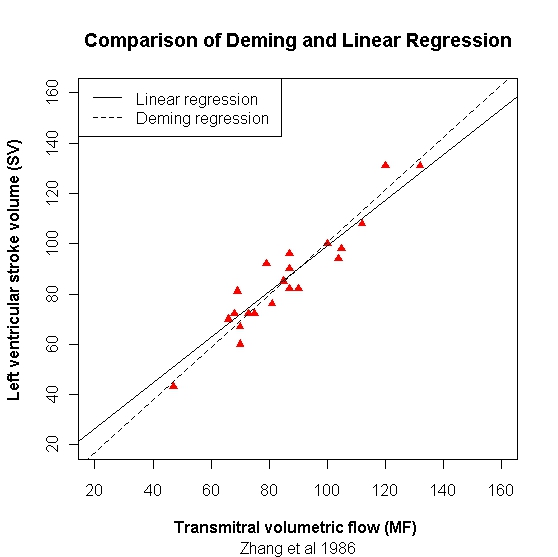
\includegraphics[width=130mm]{images/ZhangDeming.jpeg}
		\caption{Deming Regression For Zhang's Data}\label{ZhangDeming}
	\end{figure}
	
	Deming's Regression suffers from some crucial drawback. Firstly it
	is computationally complex, and it requires specific software
	packages to perform calculations.Secondly it is uninformative
	about the comparative precision of two methods of measurement.
	Most importantly \citet{CarollRupert} states that Deming's
	regression is acceptable only when the precision ratio ($\lambda$,
	in their paper as $\eta$) is correctly specified ,but in practice
	this is often not the case, with the $\lambda$ being
	underestimated.
	\newpage
	%%%%%%%%%%%%%%%%%%%%%%%%%%%%%%%%%%%%%%%%%%%%%%%%%%%%%%%%%%%%%%%%%%%%%%%%%%%%%%%%%%%%%%%%%%%%%%%%%%%%%%%%%%%%%%%%%%
	

\chapter{Model Diagnostics}
%---------------------------------------------------------------------------%
%1.1 Introduction to Influence Analysis
%1.2 Extension of techniques to LME Models
%1.3 Residual Diagnostics
%1.4 Standardized and studentized residuals
%1.5 Covariance Parameters
%1.6 Case Deletion Diagnostics
%1.7 Influence Analysis
%1.8 Terminology for Case Deletion
%1.9 Cook's Distance (Classical Case)
%1.10 Cook's Distance (LME Case)
%1.11 Likelihood Distance
%1.12 Other Measures
%1.13 CPJ Paper
%1.14 Matrix Notation of Case Deletion
%1.15 CPJ's Three Propositions
%1.16 Other measures of Influence
\tableofcontents
%===========================================================================%
\newpage

\subsection*{Abstract}
This chapter is broken into two parts. The first part is a review of diagnostics methods for linear models, intended to acquaint the reader with the subject, and also to provide a basis for material covered in the second part. Particular attention is drawn to graphical methods.

The second part of the chapter looks at diagnostics techniques for LME models, firsly covering the theory, then proceeding to a discussion on 
implementing these using \texttt{R} code.

While a substantial body of work has been developed in this area, there is still areas worth exploring. 
In particular the development of graphical techniques pertinent to LME models should be looked at.




%\section{Introduction (Page 1)}
%
%Linear models for uncorrelated data have well established measures to gauge the influence of one or more
%observations on the analysis. For such models, closed-form update expressions allow efficient computations
%without refitting the model. 
%
%
%When similar notions of statistical influence are applied to mixed models,
%things are more complicated. Removing data points affects fixed effects and covariance parameter estimates.
%Update formulas for “\textit{leave-one-out}” estimates typically fail to account for changes in covariance
%parameters. 
%
%Moreover, in repeated measures or longitudinal studies, one is often interested in multivariate
%influence, rather than the impact of isolated points. 

% This paper examines extensions of influence measures
% in linear mixed models and their implementation in the MIXED procedure.









\newpage
%=========================================================================%
\section{Model Validation Framework}
%\section{Model Validation using Residual Diagnostics}
In statistical modelling, the process of model validation is a critical step of model fitting process, but also a step that is too often overlooked. A very simple procedure is to examine commonly-used
metrics, such as the $R^2$ value. However, using a small handful of simple measures and methods is insufficient to properly assess the quality of a fitted model. To do so properly, a full and comprehensive
analysis that tests of all of the assumptions, as far as possible, must be carried out.

%=========================================================================%
%\subsection{Model Validation Framework}
%In classical linear models, this examination of model-data agreement has traditionally revolved around
\citet{schab} describes the model validatin framework as comprised of the following tasks
\begin{itemize}
	\item  overall measures of goodness-of-fit
	\item the informal, graphical examination of estimates of model errors to assess the quality of distributional
	assumptions: residual analysis
	
	
	\item the quantitative assessment of the inter-relationship of model components; for example, collinearity 	diagnostics
	\item the qualitative and quantitative assessment of influence of cases on the analysis, i.e. influence analysis.
\end{itemize}
%The sensitivity of a model is studied through measures that express its stability under perturbations. You
%are not interested in a model that is either overly stable or overly sensitive. Changes in the data or model
%components should produce commensurate changes in the model output. The difficulty is to determine
%when the changes are substantive enough to warrant further investigation, possibly leading to a reformulation
%of the model or changes in the data (such as dropping outliers).

% This paper is primarily concerned with stability of linear mixed models to perturbations of the data; that is, with influence analysis.
%========================================================================================================= %
%\subsection{Residual}



%========================================================================================================= %
%\subsection{Residual Analysis}

Residual analysis is a widely used model validation technique. A residual is simply the difference between an observed value and the corresponding fitted value, as predicted by the model. The rationale is that, if the model is properly fitted to the model, then the residuals would approximate the random errors that one should expect.
that is to say, if the residuals behave randomly, with no discernible trend, the model has fitted the data well. If some sort of non-random trend is evident in the model, then the model can be considered to be poorly fitted.

%========================================================================================================= %
%\subsection{Introduction}
%A statistical model, whether of the fixed-effects or mixed-effects variety, represents how you think your data were generated. 
%Following model specification and estimation, it is of interest to explore the model-data
%agreement by raising questions such as

Statistical software environments, such as the \texttt{R} Programming language, provides a suite of tests and graphical procedure sfor appraising a fitted linear model, with several 
of these procedures analysing the model residuals.

For LME models the matter of residual is more complex. \citet{schab} describes two types
of residuals, marginal residuals and conditional residuals. A marginal residual is the difference between the observed data and the estimated marginal mean. A conditional residual is the
difference between the observed data and the predicted value of
the observation. In a model without random effects, both sets of
residuals coincide. We shall revert to this matter in due course.

Further to the analysis of residuals, \citet{schab} recommends the examination of the following questions.
\begin{itemize}
	\item Does the model-data agreement support the model assumptions?
	\item Should model components be refined, and if so, which components? For example, should regressors
	be added or removed, and is the covariation of the observations modeled properly?
	\item Are the results sensitive to model and/or data? Are individual data points or groups of cases particularly
	influential on the analysis?
\end{itemize}



%========================================================================================================= %
\subsection{Outliers and Leverage}


The question of whether or not a point should be considered an outlier must also be addressed. An outlier is an observation whose true value is unusual given its value on the predictor variables. The leverage of an observation is a further consideration. Leverage describes an observation with an extreme value on a predictor variable is a point with high leverage. High leverage points can have a great amount of effect on the estimate of regression coefficients.
% - Leverage is a measure of how far an independent variable deviates from its mean.

Influence can be thought of as the product of leverage and outlierness. An observation is said to be influential if removing the observation substantially changes the estimate of the regression coefficients. The \texttt{R} programming language has a variety of methods used to study each of the aspects for a linear model. While linear models and GLMS can be studied with a wide range of well-established diagnostic technqiues, the choice of methodology is much more restricted for the case of LMEs.

%---------------------------------------------------------------------------%
%\newpage
%\section{Residual diagnostics} %1.3
For classical linear models, residual diagnostics are typically conducted using a plot of the observed residuals and the predicted values. A visual inspection for the presence of trends inform the analyst on the validity of distributional assumptions, and to detect outliers and influential observations.

\section{Case Deletion Diagnostics}

Since the pioneering work of Cook in 1977, deletion measures have been applied to many statistical models for identifying influential observations. Case-deletion diagnostics provide a useful tool for identifying influential observations and outliers.

The key to making deletion diagnostics useable is the development of efficient computational formulas, allowing one to obtain the \index{case deletion diagnostics} case deletion diagnostics by making use of basic building blocks, computed only once for the full model.

The computation of case deletion diagnostics in the classical model is made simple by the fact that estimates of $\beta$ and $\sigma^2$, which exclude the $i-$th observation, can be computed without re-fitting the model. %\subsection{Terminology for Case Deletion diagnostics} %1.8

\citet{preisser} describes two type of diagnostics. When the set consists of only one observation, the type is called
`\textit{observation-diagnostics}'. For multiple observations, Preisser describes the diagnostics as `\textit{cluster-deletion}' diagnostics. When applied to LME models, such update formulas are available only if one assumes that the covariance parameters are not affected by the removal of the observation in question. However, this is rarely a reasonable assumption.



%--------------------------------------%
\subsection{Extension of Diagnostic Methods to LME models}

\citet{CPJ} noted the case deletion diagnostics techniques had not been applied to linear mixed effects models and seeks to develop methodologies in that respect. \citet{CPJ} develops these techniques in the context of REML.

\citet{CPJ} develops \index{case deletion diagnostics} case deletion diagnostics, in particular the equivalent of \index{Cook's distance} Cook's distance, a well-known metric, for diagnosing influential observations when estimating the fixed effect parameters and variance components. Deletion diagnostics provide a means of assessing the influence of an observation (or groups of observations) on inference on the estimated parameters of LME models. We shall provide a fuller discussion of Cook's distance in due course.


\citet{Demi} extends several regression diagnostic techniques commonly used in linear regression, such as leverage, infinitesimal influence, case deletion diagnostics, Cook's distance, and local influence to the linear mixed-effects model. In each case, the proposed new measure has a direct interpretation in terms of the effects on a parameter of interest, and reduces to the familiar linear regression measure when there are no random effects. 

The new measures that are proposed by \citet{Demi} are explicitly defined functions and do not require re-estimation of the model, especially for cluster deletion diagnostics. The basis for both the cluster deletion diagnostics and Cook's distance is a generalization of Miller's simple update formula for case deletion for linear models. Furthermore \citet{Demi} shows how Pregibon's infinitesimal case deletion diagnostics is adapted to the linear mixed-effects model. 
%A simple compact matrix formula is derived to assess the local influence of the fixed-effects regression coefficients. 


%
%
%\section{Case Deletion Diagnostics for LME models} %1.6
%
%Data from single individuals, or a small group of subjects may influence non-linear mixed effects model selection. Diagnostics routinely applied in model building may identify such individuals, but these methods are not specifically designed for that purpose and are, therefore, not optimal. 

\citet{Demi} proposes two likelihood-based diagnostics for identifying individuals that can influence the choice between two competing models.


\subsection*{Cook's distance}
In the study of Linear model diagnostics, Cook proposed a measure that combines the information of leverage and residual of the observation, now known simply as the Cook's Distance. \citet{CPJ} would later adapt the Cook's distance measure for the analysis of LME models.



%---------------------------------------------------------------------------%

\section{Analysis of  Influence}

\subsection{Influence Analysis for LME Models} %1.1.3
The linear mixed effects model is a useful methodology for fitting a wide range of models. However, linear mixed effects models are known to be sensitive to outliers. \citet{CPJ} advises that identification of outliers is necessary before conclusions may be drawn from the fitted model.

Standard statistical packages concentrate on calculating and testing parameter estimates without considering the diagnostics of the model.The assessment of the effects of perturbations in data, on the outcome of the analysis, is known as statistical influence analysis. Influence analysis examines the robustness of the model. Influence analysis methodologies have been used extensively in classical linear models, and provided the basis for methodologies for use with LME models.
Computationally inexpensive diagnostics tools have been developed to examine the issue of influence \citep{Zewotir}.
%Studentized residuals, error contrast matrices and the inverse of the response variance covariance matrix are regular components of these tools.


%-------------------------------------------------------------------------------------------------------------------------------------%
\section{Zewotir Measures of Influence in LME Models}%2.2
%Zewotir page 161
\citet{Zewotir} describes a number of approaches to model diagnostics, investigating each of the following;
\begin{itemize}
	\item Variance components
	\item Fixed effects parameters
	\item Prediction of the response variable and of random effects
	\item likelihood function
\end{itemize}

\citet{Zewotir} lists several established methods of analyzing influence in LME models. These methods include \begin{itemize}
	\item Cook's distance for LME models,
	\item \index{likelihood distance} likelihood distance,
	\item the variance (information) ration,
	\item the \index{Cook-Weisberg statistic} Cook-Weisberg statistic,
	\item the \index{Andrews-Prebigon statistic} Andrews-Prebigon statistic.
\end{itemize}




%---------------------------------------------------------------------------%
\newpage
\section{Matrix Notation for Case Deletion} %1.14

\subsection{Case deletion notation} %1.14.1

For notational simplicity, $\boldsymbol{A}(i)$ denotes an $n \times m$ matrix $\boldsymbol{A}$ with the $i$-th row
removed, $a_i$ denotes the $i$-th row of $\boldsymbol{A}$, and $a_{ij}$ denotes the $(i, j)-$th element of $\boldsymbol{A}$.
%
%\subsection{Partitioning Matrices} %1.14.2
%Without loss of generality, matrices can be partitioned as if the $i-$th omitted observation is the first row; i.e. $i=1$.



\subsection{Further Assumptions of Linear Models}

As with fitted models, the assumption of normality of residuals and homogeneity of variance is applicable to LMEs also. 

%--------------------------------------%


Homoscedascity is the technical term to describe the variance of the
residuals being constant across the range of predicted values.
Heteroscedascity is the converse scenario : the variance differs along
the range of values.

%--Marginal and Conditional Residuals

%\subsection{INFLUENCE DIAGNOSTICS IN THE MIXED PROCEDURE}
%Key to the implementations of influence diagnostics in the MIXED procedure is the attempt to quantify
%influence, where possible, by drawing on the basic definitions of the various statistics in the classical linear
%model. 

On occasion, quantification is not possible. Assume, for example, that a data point is removed
and the new estimate of the G matrix is not positive definite. This may occur if a variance component
estimate now falls on the boundary of the parameter space. Thus, it may not be possible to compute certain
influence statistics comparing the full-data and reduced-data parameter estimates. However, knowing that
a new singularity was encountered is important qualitative information about the data point’s influence on
the analysis.

The basic procedure for quantifying influence is simple:

\begin{enumerate}
	\item Fit the model to the data and obtain estimates of all parameters.
	\item Remove one or more data points from the analysis and compute updated estimates of model parameters.
	\item Based on full- and reduced-data estimates, contrast quantities of interest to determine how the absence
	of the observations changes the analysis.
\end{enumerate}
We use the subscript (U) to denote quantities obtained without the observations in the set U. For example,
%βb
(U) denotes the fixed-effects “\textit{\textbf{leave-U-out}}” estimates. Note that the set U can contain multiple observations.


%===================================================================================
If the global measure suggests that the points in U are influential, you should next determine the nature of
that influence. In particular, the points can affect
\begin{itemize}
	\item the estimates of fixed effects
	\item the estimates of the precision of the fixed effects
	\item the estimates of the covariance parameters
	\item the estimates of the precision of the covariance parameters
	\item fitted and predicted values
\end{itemize}

It is important to further decompose the initial finding to determine whether data points are actually troublesome.
Simply because they are influential “somehow”, should not trigger their removal from the analysis or
a change in the model. For example, if points primarily affect the precision of the covariance parameters
without exerting much influence on the fixed effects, then their presence in the data may not distort hypothesis
tests or confidence intervals about $\beta$.
%They will only do so if your inference depends on an estimate of the
%precision of the covariance parameter estimates, as is the case for the Satterthwaite and Kenward-Roger
%degrees of freedom methods and the standard error adjustment associated with the DDFM=KR option.

%------------------------------------------------------------%
\subsection{Summary of Paper}
%Summary of Schabenberger
Standard residual and influence diagnostics for linear models can be extended to LME models.
The dependence of the fixed effects solutions on the covariance parameters has important ramifications on the perturbation analysis.	
Calculating the studentized residuals-And influence statistics whereas each software procedure can calculate both conditional and marginal raw residuals, only SAs Proc Mixed is currently the only program that provide studentized residuals Which ave preferred for model diagnostics. The conditional Raw residuals ave not well suited to detecting outliers as are the studentized conditional residuals. (schabenbege r)


LME are flexible tools for the analysis of clustered and repeated measurement data. LME extend the capabilities of standard linear models by allowing unbalanced and missing data, as long as the missing data are MAR. Structured covariance matrices for both the random effects G and the residuals R. missing at Random.

A conditional residual is the difference between the observed valve and the predicted valve of a dependent variable- Influence diagnostics are formal techniques that allow the identification observation that heavily influence estimates of parameters.
To alleviate the problems with the interpretation of conditional residuals that may have unequal variances, we consider sealing.
Residuals obtained in this manner ave called studentized residuals.



%---------------------------------------------------------------%
\section{Schabenberger: Summary and Conclusions}
\begin{itemize}
	\item Standard residual and influence diagnostics for linear models can be extended to linear mixed models. The dependence of fixed-effects solutions on the covariance parameter estimates has important ramifications in perturbation analysis. 
	\item To gauge the full impact of a set of observations on the analysis, covariance parameters need to be updated, which requires refitting of the model. 
	\item The experimental INFLUENCE option of the MODEL statement in the MIXED procedure (SAS 9.1) enables you to perform iterative and noniterative influence analysis for individual observations and sets of observations.
	
	\item The conditional (subject-specific) and marginal (population-averaged) formulations in the linear mixed model enable you to consider conditional residuals that use the estimated BLUPs of the random effects, and marginal residuals which are deviations from the overall mean. 
	\item Residuals using the BLUPs are useful to diagnose whether the random effects components in the model are specified correctly, marginal residuals are useful to diagnose the fixed-effects components. 
	\item Both types of residuals are available in SAS 9.1 as an experimental option of the MODEL statement in the MIXED procedure.
	
	\item It is important to note that influence analyses are performed under the assumption that the chosen model is correct. Changing the model structure can alter the conclusions. Many other variance models have been fit to the data presented in the repeated measures example. You need to see the conclusions about which model component is affected in light of the model being fit.
	%	\item  For example, modeling these data with a random intercept and random slope for each child or an unstructured covariance matrix will affect your conclusions about which children are influential on the analysis and how this influence manifests itself.
\end{itemize}











% Diagnostics with nlmeU

\section*{Leave-One-Out Diagnostics with \texttt{lmeU}}
Galecki et al provide a brief the matter of LME influence diagnostics in their book.

The command \texttt{lmeU} fits a model with a particular subject removed. The identifier of the subject to be removed is passed as the only argument

A plot ofthe per-observation diagnostics individual subject log-likelihood contributions can be rendered.

\subsubsection*{The addition of an extra factor}


%=========================================================================%


Interaction terms are featured in ANOVA designs.

%=========================================================================%
My search just now found no mention of Cook's distance or influence measures.  

The closest I found was an unanswered question on this from 
April 2003 (http://finzi.psych.upenn.edu/R/Rhelp02a/archive/4797.html).

Beyond that, there is an excellent discussion of "Examining a Fitted Model" in Sec. 4.3 (pp. 174-197) of Pinheiro and Bates (2000) 
Mixed-Effects Models in S and S-Plus (Springer).  

Pinheiro and Bates decided NOT to include plots of Cook's distance among the many diagnostics they did provide.  
However, 'plot(fit.lme)' plots 'standardized residuals' vs. predicted or 'fitted values'.  
Wouldn't points with large influence stand apart from the crowd in terms of 'fitted value'?

Of course, there are many things other one could do to get at related information, including reading the code for 'influence' and 'lme', and 
figure out from that how to write an 'influence' method for an 'lme' object. 


%============================================================================%

\section{Paired T tests}
This method can be applied to test for statisitcally significant
deviations in bias. This method can be potentially misused for
method comparison studies.
\\It is a poor measure of agreement when the rater's measurements
are perpendicular to the line of equality[Hutson et al]. In this
context, an average difference of zero between the two raters, yet
the scatter plot displays strong negative correlation.

\subsection*{Components in assessing agreement}

\begin{enumerate}
\item The degree of linear relationship between the two sets \item
The amount of bias as represented by the difference in the
means\item The Differences in the two variances.
\end{enumerate}

\section{Methods of assessing agreement}

\begin{enumerate}
\item Pearson's Correlation Coefficient\item Intraclass
correlation coefficient \item Bland Altman Plot \item Bartko's
Ellipse (1994) \item Blackwood Bradley Test \item Lin's
Reproducibility Index \item Luiz Step function
\end{enumerate}

Bland and Altman attend to the issue of repeated measures in
$1996$.

Repeated measurements on several subjects can be used to quantify
measurement error, the variation between measurements of the same
quantity on the same individual.

Bland and Altman discuss two metrics for measurement error; the
within-subject standard deviation ,and the correlation
coefficient.

The above plot incorporates both the conventional limits of
agreement ( the inner pair of dashed lines), the `t' limits of
agreement ( the outer pair of dashed lines) centred around the
inter-method bias (indicated by the full line). This plot is
intended for expository purposes only, as the sample size is
small.





\subsection{Equivalence and Interchangeability}
Limits of agreement are intended to analyse equivalence. How this
is assessed is the considered judgement of the practitioner. In
\citet{BA86} an example of good agreement is cited. For two
methods of measuring `oxygen saturation', the limits of agreement
are calculated as (-2.0,2.8).A practitioner would ostensibly find
this to be sufficiently narrow.

If the limits of agreement are not clinically important, which is
to say that the differences tend not to be substantial, the two
methods may be used interchangeably. \citet{DunnSEME} takes issue
with the notion of `equivalence', remarking that while agreement
indicated equivalence, equivalence does not reflect agreement.





\chapter{Appendix}


\section*{Bayesian BA - Philip J Schluter}
Bayesian Bland Altman Approaches
%================================%
A multivariate hierarchical Bayesian approach to measuring agreement in repeated
measurement method comparison studies

*http://www.biomedcentral.com/1471-2288/9/6*



\subsection*{Background}
Assessing agreement in method comparison studies depends on two fundamentally important components; validity (the between method agreement) and reproducibility (the within method agreement). 

The Bland-Altman limits of agreement technique is one of the favoured approaches in medical literature for assessing between method validity. However, few researchers have adopted this approach for the assessment of both validity and reproducibility. 

This may be partly due to a lack of a flexible, easily implemented and readily available statistical machinery to analyse repeated measurement method comparison data.

\textbf{Methods}\\
Adopting the Bland-Altman framework, but using Bayesian methods, we present this statistical machinery. Two multivariate hierarchical Bayesian models are advocated, one which assumes that the underlying values for subjects remain static (exchangeable replicates) and one which assumes that the underlying values can change between repeated measurements (non-exchangeable replicates).

\textbf{Results}\\
We illustrate the salient advantages of these models using two separate datasets that have been previously analysed and presented; 
(i) assuming static underlying values analysed using both multivariate hierarchical Bayesian models,  
(ii) assuming each subject's underlying value is continually changing quantity and analysed using the non-exchangeable replicate multivariate hierarchical Bayesian model.  

\textbf{Conclusion}
These easily implemented models allow for full parameter uncertainty, simultaneous method comparison, handle unbalanced or missing data, and provide estimates and credible regions for all the parameters of interest. Computer code for the analyses in also presented, provided in the freely available and currently cost free software package WinBUGS.
<hr>

\section*{Bayesian Approach}
A multivariate hierarchical Bayesian approach to measuring agreement in repeated measurement method comparison studies
PJ Schluter - BMC medical research methodology, 2009 - biomedcentral.com

\begin{itemize}
	\item Assessing agreement in method comparison studies depends on two fundamentally important 
	components; validity (the between method agreement) and reproducibility (the within method 
	agreement). 
	\item The Bland-Altman limits of agreement technique is one of the f
\end{itemize}

%========================%
\section{Escaramis}
% Escaramis et al 2010
% http://www.biomedcentral.com/1471-2288/10/31/
%-----------------------------------------------------%
\subsection{Background}
In an agreement assay, it is of interest to evaluate the degree of agreement between the different methods (devices, instruments or observers) used to measure the same characteristic. We propose in this study a technical simplification for inference about the total deviation index (TDI) estimate to assess agreement between two devices of normally-distributed measurements and describe its utility to evaluate inter- and intra-rater agreement if more than one reading per subject is available for each device.

\subsection{Methods}
We propose to estimate the TDI by constructing a probability interval of the difference in paired measurements between devices, and thereafter, we derive a tolerance interval (TI) procedure as a natural way to make inferences about probability limit estimates. We also describe how the proposed method can be used to compute bounds of the coverage probability.

\subsection{Results}
The approach is illustrated in a real case example where the agreement between two instruments, a handle mercury sphygmomanometer device and an OMRON 711 automatic device, is assessed in a sample of 384 subjects where measures of systolic blood pressure were taken twice by each device. A simulation study procedure is implemented to evaluate and compare the accuracy of the approach to two already established methods, showing that the TI approximation produces accurate empirical confidence levels which are reasonably close to the nominal confidence level.

\subsection{Conclusions}
The method proposed is straightforward since the TDI estimate is derived directly from a probability interval of a normally-distributed variable in its original scale, without further transformations. Thereafter, a natural way of making inferences about this estimate is to derive the appropriate TI. Constructions of TI based on normal populations are implemented in most standard statistical packages, thus making it simpler for any practitioner to implement our proposal to assess agreement.

%-----------------------------------------------------%
%PAGE 3 of 12 COLUMN 1
Lin defined the TDI as the boundary, $\kappa_P$ which capyures a large proportion $p$ of paired based differences from 
two devices or observers within the boundary.

The value of $\kappa_P$ that yeilds $P(|D| <\kappa_p) = p$ where D is the paired-difference variate.

%-----------------------------------------------------%
%PAGE 3 of 12 COLUMN 2

\[ \kappa_P = F^{-1}(p) = \sigma_D \sqrt{\chi^2(p,1,\mu^2_D/\sigma^2_d) }  \]

\[ \kappa_P = Z_{\frac{1+p}{2}} \| \varepsilon\| \]

%-----------------------------------------------------%

%PAGE 5 of 12 COLUMN 1

Tolerance Interval around the TDI estimate

\[ \hat{\kappa_p} = \hat{\mu}_D = Z_{p_i}\sigma_d \]

%-----------------------------------------------------%

%PAGE 5 of 12 COLUMN 2
Coverage Probability is another user friendly measure of agrre,ment which is related to the computation of the TDI.

\section{Schabenberger}

\emph{schab} examines the use and implementation of
influence measures in LME models.

Influence is understood to be the ability of a single or multiple
data points, through their presences or absence in the data, to
alter important aspects of the analysis, yield qualitatively
different inferences, or violate assumptions of the statistical
model (\textit{schabenberger}).

Outliers are the most noteworthy data points in an analysis, and
an objective of influence analysis is how influential they are,
and the manner in which they are influential.

\emph{schab} describes a simple procedure for quantifying
influence. Firstly a model should be fitted to the data, and
estimates of the parameters should be obtained. The second step is
that either single of multiple data points, specifically outliers,
should be omitted from the analysis, with the original parameter
estimates being updated. 

This is known as `\textit{leave one out \ leave k
	out}' analysis. The final step of the procedure is comparing the
sets of estimates computed from the entire and reduced data sets
to determine whether the absence of observations changed the
analysis.

\textit{schabenberger} notes that it is not always possible to
derive influence statistics necessary for comparing full- and
reduced-data parameter estimates. 

%
%\begin{abstract}
%	\noindent This paper reviews the use of diagnostic measures for LME models in SAS. This text has been widely cited by texts that don't deal with SAS implementations.
%\end{abstract}
%

%==================================================================================================== %

In recent years, mixed models have become invaluable tools in the analysis of experimental and observational
data. In these models, more than one term can be subject to random variation. Mixed model
technology enables you to analyze complex experimental data with hierarchical random processes, temporal,
longitudinal, and spatial data, to name just a few important applications. 
%
%\subsection{Stating the LME Model}
%The general linear mixed
%model is
%\[
%Y = X\beta + Zu + \varepsilon\]
%where Y is a $(n\times1)$ vector of observed data, X is an $(n\times p)$ fixed-effects design or regressor matrix of rank
%k, Z is a $(n \times g)$ random-effects design or regressor matrix, $u$ is a $(g \times 1)$ vector of random effects, and $\varepsilon$ is
%an $(n\times1)$ vector of model errors (also random effects). The distributional assumptions made by the MIXED
%procedure are as follows: γ is normal with mean 0 and variance G; $\varepsilon$ is normal with mean 0 and variance
%R; the random components $u$ and $\varepsilon$ are independent. Parameters of this model are the fixed-effects β and
%all unknowns in the variance matrices G and R. The unknown variance elements are referred to as the
%covariance parameters and collected in the vector $theta$.
%===========================================================================%

\emph{schab} remarks that the concept of critiquing the model-data agreement applies in mixed models in the same way as in linear
fixed-effects models. In fact, because of the more complex model structure, you can argue that model and
data diagnostics are even more important. For example, you are not only concerned with capturing the
important variables in the model. You are also concerned with ``distributing” them correctly between the
fixed and random components of the model. The mixed model structure presents unique and interesting
challenges that prompt us to reexamine the traditional ideas of influence and residual analysis.
%==========================================================================%
%This paper presents the extension of traditional tools and statistical measures for influence and residual
%analysis to the linear mixed model and demonstrates their implementation in the MIXED procedure (experimental
%features in SAS 9.1). The remainder of this paper is organized as follows. The “Background” section
%briefly discusses some mixed model estimation theory and the challenges to model diagnosis that result
%from it.

%	 The diagnostics implemented in the MIXED procedure are discussed in the “Residual Diagnostics
%	in the MIXED Procedure” section (page 3) and the “Influence Diagnostics in the MIXED Procedure” section
%	(page 5). The syntax options and suboptions you use to request the various diagnostics are briefly sketched
%	in the “Syntax” section (page 9). The presentation concludes with an example.
%	
%	
%====================================================================================================================%



\section{Hawkins : Diagnostics for conformity of paired quantitative measurements}

\begin{itemize}
	\item Matched pairs data arise in many contexts – in case-control clinical trials, for example, and from cross-over designs. They also arise in experiments to verify the equivalence of quantitative assays. This latter use (which is the main focus of this paper) raises difficulties not always seen in other matched pairs applications. 
	
	\item Since the designs deliberately vary the analyte levels over a wide range, issues of variance dependent on mean, calibrations of differing slopes, and curvature all need to be added to the usual model assumptions such as normality. 
	
	\item Violations in any of these assumptions invalidate the conventional matched pairs analysis. 
	
	\item A graphical method, due to Bland and Altman, of looking at the relationship between the average and the difference of the members of the pairs is shown to correspond to a formal testable regression model. 
	
	\item Using standard regression diagnostics, one may detect and diagnose departures from the model assumptions and remedy them – for example using variable transformations. Examples of different common scenarios and possible approaches to handling them are shown.
\end{itemize}
%====================================%

% 1. Problem Description
% 2. A Statistical Formulation
%    2.1 Regression Methods for Testing Equivalence
%    2.2 Matched Pair Analysis
% 3. Regression of Differences on Sums
%    3.1 Use of Formal regression Diagnostics
% 4. Examples
%    4.1 Example 1
%    4.2 Detection and Cure of Heteroscedascity
%    4.3 Example 2
%    4.4 Example 3
%    4.5 Example 4
%    4.6 Example 5
% 5. Precepts for Design
% 6. Conclusion


%====================================%
A multi-Rate nonparametric test of agreement and corresponding agreement plot

- Published in: Computational Statistics and Data Analysis 54(2010)109-119
- Author: Alan D. Hutson, University of Buffalo



This approach takes advantage of readily avilable tests of uniformity found in most statistical software packages.
Such tests include the KS d statistic, the Anderson Darling Statistic and the Cramer-Von Mises statistical test for univariate data.

An important aspect of this approach is the "Agreement Region".



\section*{Roy Test}

Roy’s Tests (Roy 2009)
%=============================%
Roy 2009 devised an LME based Testing approach to the MCS problem, based on earlier work by Hamlett et al. 
Roy 2009 presents a series of three formal hypothesis tests for assessing agreement between two methods of measurement.
Roy also alludes to some of the current shortcomings of the approach.

%%%% Components of Test

Comparing different model specifications with LRT tests

%%%% Papers:
- Roy 2007
- Roy 2009
- Hamlett et al.
- Roy Leiva 2011



Conventionally LME models can be tested using Likelihood Ratio Tests, wherein a reference model is compared to a nested model.
\begin{verbatim}
> Ref.Fit = lme(y ~ meth-1, data = dat,   #Symm , Symm#
+     random = list(item=pdSymm(~ meth-1)), 
+     weights=varIdent(form=~1|meth),
+     correlation = corSymm(form=~1 | item/repl), 
+     method="ML")
\end{verbatim}
Roy(2009) presents two nested models that specify the condition of equality as required, with a third nested model for an additional test. There three formulations share the same structure, and can be specified by making slight alterations of the code for the Reference Model.
\begin{verbatim}
Nested Model (Between-Item Variability)
> NMB.fit  = lme(y ~ meth-1, data = dat,   #CS , Symm#
+     random = list(item=pdCompSymm(~ meth-1)),
+     correlation = corSymm(form=~1 | item/repl), 
+     method="ML")
\end{verbatim}



\begin{verbatim}
Nested Model (Within –item Variability)
> NMW.fit = lme(y ~ meth-1, data = dat,   #Symm , CS# 
+     random = list(item=pdSymm(~ meth-1)),
+     weights=varIdent(form=~1|meth), 
+     correlation = corCompSymm(form=~1 | item/repl), 
+     method="ML")
\end{verbatim}


Nested Model (Overall Variability)
Additionally there is a third nested model, that can be used to test overall variability, substantively a a joint test for between-item and within-item variability. The motivation for including such a test in the suite is not clear, although it does circumvent the need for multiple comparison procedures in certain circumstances, hence providing a simplified procedure for non-statisticians.
\begin{verbatim}
> NMO.fit = lme(y ~ meth-1, data = dat,   #CS , CS# 
+     random = list(item=pdCompSymm(~ meth-1)), 
+     correlation = corCompSymm(form=~1 | item/repl), 
+     method="ML")
\end{verbatim}

ANOVAs  for  Original Fits
The likelihood Ratio test is very simple to implement in R. All that is required it to specify the reference model and the relevant nested mode as arguments to the command anova().
The figure below displays the three tests described by Roy (2009).
\begin{verbatim}
> testB    = anova(Ref.Fit,NMB.fit)                          # Between-Subject Variabilities
> testW   = anova(Ref.Fit,NMW.fit)                        # Within-Subject Variabilities
> testO     = anova(Ref.Fit,NMO.fit)                        # Overall Variabilities
\end{verbatim}
\newpage
\section{Profile Function with "lmer"}

The profile() function for lmer models is now available in the latest version of lme4, to be installed by typing:

install.packages("lme4",repos="http://r-forge.r-project.org")

also

The mle function from the stats4 package is a wrapper of optim, which makes it quite easy to produce 
profile likelihood computations. 

See help("profile,mle-method", package = "stats4") for more information.

%----------------%

http://people.upei.ca/hstryhn/stryhn208.pdf

The profile likelihood (or likelihood or likelihood ratio) methid is applicable to 
all likelihood based statstical analysis and is generally less sensitive to the difficulties
encountered by walkd-Tyoe CIs.



\section{Turkan's LMEs}
% Influence Analysis in the LME Models
% Turkan and Toktamus
% Pakistan Journal of Statistics;2012, Vol. 28 Issue 3, p341

% - http://www.tandfonline.com/doi/abs/10.1080/03610920903564727?journalCode=lsta20#.VHj9vfmsXE4

The linear mixed model is considerably sensitive to outliers and influential observations. 
It is known that outliers and influential observations affect substantially the results of analysis. 
So it is very important to be aware of these observations. 

Some diagnostics which are analogue of diagnostics in multiple linear regression were developed to detect 
outliers and influential observations in the linear mixed model. 
\emph{
	In this paper, the new diagnostic measure which is analogue of the Pena's influence statistic is developed for 
	the linear mixed model.
}
\newpage
%-----------------------------------------------------------------------------------------%

%page 341

%-----------------------------------------------------------------------------------------%
%page 342
Estimation and Building blacks in LME models

%-----------------------------------------------------------------------------------------%
%page 343

\[ \hat{u} = DZ^{T}H^{-1}(y-X\hat{\beta}) \]

\[ \hat{y} = (I_n -  H^{-1})y + H^{-1}X\hat{\beta}\]

%-----------------------------------------------------------------------------------------%
%page 345

The proposed diagnostic Measure.

%-----------------------------------------------------------------------------------------%
% http://halweb.uc3m.es/esp/Personal/personas/dpena/articles/TECHanews2005.pdf

\subsection{Ordinary Least Product Regression}
\citet{ludbrook97} states that the grouping structure can be
straightforward, but there are more complex data sets that have a
hierarchical(nested) model.
\\
\\
Observations between groups are independent, but observations
within each groups are dependent because they belong to the same
subpopulation. Therefore there are two sources of variation:
between-group and within-group variance.
 \vspace{5 mm} \noindent Mean correction is a method of reducing
bias.







\subsection{A regression based approach based on Bland Altman Analysis}
Lu et al used such a technique in their comparison of DXA
scanners. They also used the Blackwood Bradley test. However it
was shown that, for particular comparisons,  agreement between
methods was indicated according to one test, but lack of agreement
was indicated by the other.


\section{Measurement Error Models}
\citet{DunnSEME} proposes a measurement error model for use in
method comparison studies. Consider n pairs of measurements
$X_{i}$ and $Y_{i}$ for $i=1,2,...n$.
\begin{equation}
X_{i} = \tau_{i}+\delta_{i}\\
\end{equation}
\begin{equation}
 Y_{i} = \alpha +\beta\tau_{i}+\epsilon_{i} \nonumber
\end{equation}

In the above formulation is in the form of a linear structural
relationship, with $\tau_{i}$ and $\beta\tau_{i}$ as the true
values , and $\delta_{i}$ and $\epsilon_{i}$ as the corresponding
measurement errors. In the case where the units of measurement are
the same, then $\beta =1$.

\begin{equation}
E(X_{i}) = \tau_{i}\\
\end{equation}
\begin{equation}
E(Y_{i}) = \alpha +\beta\tau_{i} \nonumber
\end{equation}
\begin{equation}
E(\delta_{i}) = E(\epsilon_{i}) = 0 \nonumber
\end{equation}

The value $\alpha$ is the inter-method bias between the two
methods.

\begin{eqnarray}
  z_0 &=& d = 0 \\
  z_{n+1} &=& z_n^2+c
\end{eqnarray}

% http://www.jstor.org/discover/10.2307/1269550?uid=3738232&uid=2&uid=4&sid=21103552726783

% Abstract for CPJ paper
% Mixed linear models arise in many areas of application. 
% Standard estimation methods for mixed models are sensitive to bizarre observations. 
% Such influential observations can completely distort an analysis and lead to inappropriate actions and conclusions. 
% We develop case-deletion diagnostics for detecting influential observations in mixed linear models. 
% Diagnostics for both fixed effects and variance components are proposed. 
% Computational formulas are given that make the procedures feasible. 
% The methods are illustrated using examples.




\section{Work List}
\begin{enumerate}
	\item ML v REML
	\item Nested Models and LRTs
	\item Generalized Lease Squares
	\item Diagnostics
	\item Simplifying GLS
	\item Paper progression
\end{enumerate}





\newpage
%--------------------------------------------------------------------Diagnostics%
\section{Diagnostics}

%http://www.artifex.org/~meiercl/R_statistics_guide.pdf
\subsection{Identifying outliers with a LME model object}

The process is slightly different than with standard LME model objects, since the \textbf{\emph{influence}}
function does not work on lme model objects. Given \textbf{\emph{mod.lme}}, we can use the plot function to
identify outliers.
%----------------------%
\subsection{Diagnostics for Random Effects}
Empirical best linear unbiased predictors EBLUPS provide the a useful way of diagnosing random effects.

EBLUPs are also known as ``shrinkage estimators" because they tend to be smaller than the estimated effects would be if they were computed by treating a random factor as if it was fixed (West etal )

		%---------------------------------------------------------------------------%
		\newpage
		\section{Iterative and non-iterative influence analysis} %1.13
		\citet{schab} highlights some of the issue regarding implementing mixed model diagnostics.
		
		% A measure of total influence requires updates of all model parameters.
		% however, this doesnt increase the procedures execution time by the same degree.
		
		\subsection{Iterative Influence Analysis}
		
		%----schabenberger page 8
		For linear models, the implementation of influence analysis is straightforward.
		However, for LME models, the process is more complex. Update formulas for the fixed effects are available only when the covariance parameters are assumed to be known. A measure of total influence requires updates of all model parameters.
		This can only be achieved in general is by omitting observations, then refitting the model.
		
		\citet{schab} describes the choice between \index{iterative influence analysis} iterative influence analysis and \index{non-iterative influence analysis} non-iterative influence analysis.
		
		
		
		
		
		\subsection{Iterative vs Non-Iterative Influence Analysis}
		%\subsection{ITERATIVE VS. NONITERATIVE INFLUENCE ANALYSIS}
		While the basic idea of influence analysis is straightforward, the implementation in mixed models can be
		tricky. For example, update formulas for the fixed effects are available only when the covariance parameters
		are assumed to be known. At most the profiled residual variance can be updated without refitting the model.
		
		A measure of total influence requires updates of all model parameters, and the only way that this can be
		achieved in general is by removing the observations in question and refitting the model. 
		
		Because this “\textbf{bruteforce}”
		method involves iterative reestimation of the covariance parameters, it is termed \textbf{\textit{iterative influence
				analysis}}. Reliance on closed-form update formulas for the fixed effects without updating the (un-profiled)
		covariance parameters is termed a noniterative influence analysis.
		
		An iterative analysis seems like a costly, computationally intensive enterprise. If you compute iterative
		influence diagnostics for all n observations, then a total of $n + 1$ mixed models are fit iteratively. This does
		not imply, of course, that the procedure’s execution time increases n-fold. Keep in mind that
		\begin{itemize}
			\item iterative reestimation always starts at the converged full-data estimates. If a data point is not influential,
			then its removal will have little effect on the objective function and parameter estimates. Within
			one or two iterations, the process should arrive at the reduced-data estimates.
			\item if complete reestimation does require many iterations, then this is important information in itself. The
			likelihood surface has probably changed drastically, and the reduced-data estimates are moving away
		\end{itemize}
		from the full-data estimates.
%-------------------------------------------------------------------Simplifying GLS by KH -%

%---------------------------------------------------------------------------------------------------%
\newpage

\section{Two-tailed testing} A test for equality of variances, based on the likelihood Ratio test, is very simple to implement using existing methodologies. All that is required it to specify the reference model and the relevant nested mode as arguments to the command \texttt{anova()}. The output can be interpreted in the usual way.

\section{One Tailed Testing}
The approach proposed by Roy deals with the question of agreement, and indeed interchangeability, as developed by Bland and Altman's corpus of work. In the view of Dunn, a question relevant to many practitioners is which of the two methods is more precise.

The relationship between precision and the within-item and between-item variability must be established. Roy establishes the equivalence of repeatability and within-item variability, and hence precision.  The method with the smaller within-item variability can be deemed to be the more precise.

\section{Enabling One Tailed Testing}
A useful approach is to compute the confidence intervals for the ratio of within-item standard deviations (equivalent to the ratio of repeatability coefficients), which can be interpreted in the usual manner ( or alternatively, the ratio of the variances). In fact, the ratio of within-item standard deviations, with the attendant confidence interval,  can be determined using a single \texttt{R} command: \texttt{intervals()}.

Pinheiro and Bates (pg 93-95) give a description of how confidence intervals for the variance components are computed. Furthermore a complete set of confidence intervals can be computed to complement the variance component estimates.
However , to facilitate one tailed testing, What is required is the computation of the variance ratios of within-item and between-item standard deviations.

A naive approach would be to compute the variance ratios by relevant F distribution quantiles. However, the question arises as to the appropriate degrees of freedom. However, Douglas Bates has stated that an alternative approach is required (i.e. Profile Likelihoods)

\begin{quote}
	"The omission of standard errors on variance components is intentional.
	The distribution of an estimator of a variance component is highly
	skewed and obtaining an estimate of the standard deviation of a skewed
	distribution is not very useful.  A much better approach is based on
	profiling the objective function." (Douglas Bates May 2012)
\end{quote}


\section{Profile Likelihood}
Normal-based confidence intervals for a parameter of interest are inaccurate when the sampling distribution of the estimate is skewed. The technique known as profile likelihood can produce confidence intervals with better coverage. It may be used when the model includes only the variable of interest or several other variables in addition. Profile-likelihood confidence intervals are particularly useful in nonlinear models.

Profile likelihood confidence intervals are based on the log-likelihood function.  
%For a single parameter, likelihood theory shows that the 2 points 1.92 units down from the maximum of the log-likelihood function provide a $95\%$ confidence interval when there is no extrabinomial variation (i.e. c = 1)..  The value 1.92 is half of the chi-square value of 3.84 with 1 degree of freedom.

%Thus, the same confidence interval can be computed with the deviance by adding 3.84 to the minimum of the deviance function, where the deviance is the log-likelihood multiplied by -2 minus the -2 log likelihood value of the saturated model.

\section{Implementation of PL Confidence Intervals}

The suitable calculation of confidence limits for this variance ratio are to be computed using the profile likelihood approach. The \texttt{R} package \texttt{profilelikelihood} will be assessed for feasibility, particularly the command \texttt{profilelikelihood.lme()}



%http://cran.r-project.org/web/packages/ProfileLikelihood/ProfileLikelihood.pdf

%http://lme4.r-forge.r-project.org/slides/2011-03-16-Amsterdam/3Profiling.pdf

%http://lme4.r-forge.r-project.org/slides/2009-07-21-Seewiesen/4PrecisionD.pdf



%---------------------------------------------------------------------------%
\newpage
\section{Extension of techniques to LME Models} %1.2

Model diagnostic techniques, well established for classical models, have since been adapted for use with linear mixed effects models.Diagnostic techniques for LME models are inevitably more difficult to implement, due to the increased complexity.

Beckman, Nachtsheim and Cook (1987) \citet{Beckman} applied the \index{local influence}local influence method of Cook (1986) to the analysis of the linear mixed model.

While the concept of influence analysis is straightforward, implementation in mixed models is more complex. Update formulae for fixed effects models are available only when the covariance parameters are assumed to be known.

If the global measure suggests that the points in $U$ are influential, the nature of that influence should be determined. In particular, the points in $U$ can affect the following

\begin{itemize}
	\item the estimates of fixed effects,
	\item the estimates of the precision of the fixed effects,
	\item the estimates of the covariance parameters,
	\item the estimates of the precision of the covariance parameters,
	\item fitted and predicted values.
\end{itemize}



%--Marginal and Conditional Residuals

\subsection{Residuals diagnostics in mixed models}

%schabenberger
The marginal and conditional means in the linear mixed model are
$E[\boldsymbol{Y}] = \boldsymbol{X}\boldsymbol{\beta}$ and
$E[\boldsymbol{Y|\boldsymbol{u}}] = \boldsymbol{X}\boldsymbol{\beta} + \boldsymbol{Z}\boldsymbol{u}$, respectively.

A residual is the difference between an observed quantity and its estimated or predicted value. In the mixed
model you can distinguish marginal residuals $r_m$ and conditional residuals $r_c$. 


\subsection{Marginal and Conditional Residuals}

A marginal residual is the difference between the observed data and the estimated (marginal) mean, $r_{mi} = y_i - x_0^{\prime} \hat{b}$
A conditional residual is the difference between the observed data and the predicted value of the observation,
$r_{ci} = y_i - x_i^{\prime} \hat{b} - z_i^{\prime} \hat{\gamma}$

In linear mixed effects models, diagnostic techniques may consider `conditional' residuals. A conditional residual is the difference between an observed value $y_{i}$ and the conditional predicted value $\hat{y}_{i} $.

\[ \hat{epsilon}_{i} = y_{i} - \hat{y}_{i} = y_{i} - ( X_{i}\hat{beta} + Z_{i}\hat{b}_{i}) \]

However, using conditional residuals for diagnostics presents difficulties, as they tend to be correlated and their variances may be different for different subgroups, which can lead to erroneous conclusions.

%1.5
%http://support.sas.com/documentation/cdl/en/statug/63033/HTML/default/viewer.htm#statug_mixed_sect024.htm






\begin{equation}
r_{mi}=x^{T}_{i}\hat{\beta}
\end{equation}

\subsection{Marginal Residuals}
\begin{eqnarray}
\hat{\beta} &=& (X^{T}R^{-1}X)^{-1}X^{T}R^{-1}Y \nonumber \\
&=& BY \nonumber
\end{eqnarray}

%---------------------------------------------------------------------------%
\newpage
\section{Standardized and studentized residuals} %1.4
%--Studentized and Standardized Residuals

To alleviate the problem caused by inconstant variance, the residuals are scaled (i.e. divided) by their standard deviations. This results in a \index{standardized residual}`standardized residual'. Because true standard deviations are frequently unknown, one can instead divide a residual by the estimated standard deviation to obtain the \index{studentized residual}`studentized residual. 

\subsection{Standardization} %1.4.1

A random variable is said to be standardized if the difference from its mean is scaled by its standard deviation. The residuals above have mean zero but their variance is unknown, it depends on the true values of $\theta$. Standardization is thus not possible in practice.

\subsection{Studentization} %1.4.2
Instead, you can compute studentized residuals by dividing a residual by an estimate of its standard deviation. 

\subsection{Internal and External Studentization} %1.4.3
If that estimate is independent of the $i-$th observation, the process is termed \index{external studentization}`external studentization'. This is usually accomplished by excluding the $i-$th observation when computing the estimate of its standard error. If the observation contributes to the
standard error computation, the residual is said to be \index{internally studentization}internally studentized.

Externally \index{studentized residual} studentized residual require iterative influence analysis or a profiled residuals variance.


\subsection{Computation}%1.4.4

The computation of internally studentized residuals relies on the diagonal entries of $\boldsymbol{V} (\hat{\theta})$ - $\boldsymbol{Q} (\hat{\theta})$, where $\boldsymbol{Q} (\hat{\theta})$ is computed as

\[ \boldsymbol{Q} (\hat{\theta}) = \boldsymbol{X} ( \boldsymbol{X}^{\prime}\boldsymbol{Q} (\hat{\theta})^{-1}\boldsymbol{X})\boldsymbol{X}^{-1} \]

\subsection{Pearson Residual}%1.4.5

Another possible scaled residual is the \index{Pearson residual} `Pearson residual', whereby a residual is divided by the standard deviation of the dependent variable. The Pearson residual can be used when the variability of $\hat{\beta}$ is disregarded in the underlying assumptions.

%---------------------------------------------------------------------------%
\newpage
\section{Covariance Parameters} %1.5
The unknown variance elements are referred to as the covariance parameters and collected in the vector $\theta$.
% - where is this coming from?
% - where is it used again?
% - Has this got anything to do with CovTrace etc?
%---------------------------------------------------------------------------%

\subsection{Methods and Measures}
The key to making deletion diagnostics useable is the development of efficient computational formulas, allowing one to obtain the \index{case deletion diagnostics} case deletion diagnostics by making use of basic building blocks, computed only once for the full model.

\citet{Zewotir} lists several established methods of analyzing influence in LME models. These methods include \begin{itemize}
	\item Cook's distance for LME models,
	\item \index{likelihood distance} likelihood distance,
	\item the variance (information) ration,
	\item the \index{Cook-Weisberg statistic} Cook-Weisberg statistic,
	\item the \index{Andrews-Prebigon statistic} Andrews-Prebigon statistic.
\end{itemize}


%-------------------------------------------------------------------------------------------------Chapter 2	------------------------%
%-------------------------------------------------------------------------------------------------------------------------------------%
%-------------------------------------------------------------------------------------------------------------------------------------%

\section{Computation and Notation } %2.3
with $\boldsymbol{V}$ unknown, a standard practice for estimating $\boldsymbol{X \beta}$ is the estime the variance components $\sigma^2_j$,
compute an estimate for $\boldsymbol{V}$ and then compute the projector matrix $A$, $\boldsymbol{X \hat{\beta}}  = \boldsymbol{AY}$.


\citet{Zewotir} remarks that $\boldsymbol{D}$ is a block diagonal with the $i-$th block being $u \boldsymbol{I}$
%--------------------------------------------------------------%

\section{Measures 2} %2.4

\subsection{Cook's Distance} %2.4.1
\begin{itemize}
	\item For variance components $\gamma$
\end{itemize}

Diagnostic tool for variance components
\[ C_{\theta i} =(\hat(\theta)_{[i]} - \hat(\theta))^{T}\mbox{cov}( \hat(\theta))^{-1}(\hat(\theta)_{[i]} - \hat(\theta))\]



\chapter{Linear Mixed Effects Models}

\section{LME models in Method comparison}
%With the greater computing power available for scientific
%analysis, it is inevitable that complex models such as linear
%mixed effects models should be applied to method comparison
%studies.







% \begin{equation}
% data here
% \end{equation}

\newpage
\section{Lai Shiao}
\citet{LaiShiao} use mixed models to determine the factors that
affect the difference of two methods of measurement using the
conventional formulation of linear mixed effects models.

If the parameter \textbf{b}, and the variance components are not
significantly different from zero, the conclusion that there is no
inter-method bias can be drawn. If the fixed effects component
contains only the intercept, and a simple correlation coefficient
is used, then the estimate of the intercept in the model is the
inter-method bias. Conversely the estimates for the fixed effects
factors can advise the respective influences each factor has on
the differences. The Proc Mixed package allows users to specify
different correlation structures of the variance components
\textbf{G} and \textbf{R}.


Oxygen saturation is one of the most frequently measured variables
in clinical nursing studies. `Fractional saturation' ($HbO_{2}$)
is considered to be the gold standard method of measurement, with
`functional saturation' ($SO_{2}$) being an alternative method.
The method of examining the causes of differences between these
two methods is applied to a clinical study conducted by
\citet{Shiao}. This experiment was conducted by 8 lab
practitioners on blood samples, with varying levels of
haemoglobin, from two donors. The samples have been in storage for
varying periods ( described by the variable `Bloodage') and are
categorized according to haemoglobin percentages(i.e
$0\%$,$20\%$,$40\%$,$60\%$,$80\%$,$100\%$). There are 625
observations in all.

\citet{LaiShiao} fits two models on this data, with the lab
technicians and the replicate measurements as the random effects
in both models. The first model uses haemoglobin level as a fixed
effects component. For the second model, blood age is added as a
second fixed factor.

\subsubsection{Single fixed effect} The first model fitted by \citet{LaiShiao} takes the
blood level as the sole fixed effect to be analyzed. The following
coefficient estimates are estimated by `Proc Mixed';
\begin{eqnarray}
\mbox{fixed effects :   } 2.5056 - 0.0263\mbox{Fhbperct}_{ijtl} \\
(\mbox{p-values :   } = 0.0054, <0.0001, <0.0001)\nonumber\\\nonumber\\
\mbox{random effects :   } u(\sigma^{2}=3.1826) + e_{ijtl}
(\sigma^{2}_{e}=0.1525, \rho= 0.6978) \nonumber\\
(\mbox{p-values :   } = 0.8113, <0.0001, <0.0001)\nonumber
\end{eqnarray}

With the intercept estimate being both non-zero and statistically
significant ($p=0.0054$), this models supports the presence
inter-method bias is $2.5\%$ in favour of $SO_{2}$. Also, the
negative value of the haemoglobin level coefficient indicate that
differences will decrease by $0.0263\%$ for every percentage
increase in the haemoglobin .

In the random effects estimates, the variance due to the
practitioners is $3.1826$, indicating that there is a significant
variation due to technicians ($p=0.0311$) affecting the
differences. The variance for the estimates is given as $0.1525$,
($p<0.0001$).

\subsubsection{Two fixed effects}
Blood age is added as a second fixed factor to the model,
whereupon new estimates are calculated;
\begin{eqnarray}
\mbox{fixed effects :   } -0.2866 + 0.1072 \mbox{Bloodage}_{ijtl}
- 0.0264\mbox{Fhbperct}_{ijtl}\nonumber\\
( \mbox{p-values :   } = 0.8113, <0.0001, <0.0001)\nonumber\\\nonumber\\
\mbox{random effects :   } u(\sigma^{2}=10.2346) + e_{ijtl}
(\sigma^{2}_{e}=0.0920, \rho= 0.5577) \nonumber\\
(\mbox{p-values :   } = 0.0446, <0.0001, <0.0001)
\end{eqnarray}


With this extra fixed effect added to the model, the intercept
term is no longer statistically significant. Therefore, with the
presence of the second fixed factor, the model is no longer
supporting the presence of inter-method bias. Furthermore, the
second coefficient indicates that the blood age of the observation
has a significant bearing on the size of the difference between
both methods ($p <0.0001$). Longer storage times for blood will
lead to higher levels of particular blood factors such as MetHb
and HbCO (due to the breakdown and oxidisation of the
haemoglobin). Increased levels of MetHb and HbCO are concluded to
be the cause of the differences. The coefficient for the
haemoglobin level doesn't differ greatly from the single fixed
factor model, and has a much smaller effect on the differences.
The random effects estimates also indicate significant variation
for the various technicians; $10.2346$ with $p=0.0446$.

\citet{LaiShiao} demonstrates how that linear mixed effects models
can be used to provide greater insight into the cause of the
differences. Naturally the addition of further factors to the
model provides for more insight into the behavior of the data.



\newpage
\section{Carstensen's Mixed Models}

\citet{BXC2004} proposes linear mixed effects models for deriving
conversion calculations similar to Deming's regression, and for
estimating variance components for measurements by different
methods. The following model ( in the authors own notation) is
formulated as follows, where $y_{mir}$ is the $r$th replicate
measurement on subject $i$ with method $m$.

\begin{equation}
y_{mir}  = \alpha_{m} + \beta_{m}\mu_{i} + c_{mi} + e_{mir} \qquad
( e_{mi} \sim N(0,\sigma^{2}_{m}), c_{mi} \sim N(0,\tau^{2}_{m}))
\end{equation}
The intercept term $\alpha$ and the $\beta_{m}\mu_{i}$ term follow
from \citet{DunnSEME}, expressing constant and proportional bias
respectively , in the presence of a real value $\mu_{i}.$
$c_{mi}$ is a interaction term to account for replicate, and
$e_{mir}$ is the residual associated with each observation.
Since variances are specific to each method, this model can be
fitted separately for each method.

The above formulation doesn't require the data set to be balanced.
However, it does require a sufficient large number of replicates
and measurements to overcome the problem of identifiability. The
import of which is that more than two methods of measurement may
be required to carry out the analysis. There is also the
assumptions that observations of measurements by particular
methods are exchangeable within subjects. (Exchangeability means
that future samples from a population behaves like earlier
samples).

%\citet{BXC2004} describes the above model as a `functional model',
%similar to models described by \citet{Kimura}, but without any
%assumptions on variance ratios. A functional model is . An
%alternative to functional models is structural modelling

\citet{BXC2004} uses the above formula to predict observations for
a specific individual $i$ by method $m$;

\begin{equation}BLUP_{mir} = \hat{\alpha_{m}} + \hat{\beta_{m}}\mu_{i} +
c_{mi} \end{equation}. Under the assumption that the $\mu$s are
the true item values, this would be sufficient to estimate
parameters. When that assumption doesn't hold, regression
techniques (known as updating techniques) can be used additionally
to determine the estimates. The assumption of exchangeability can
be unrealistic in certain situations. \citet{BXC2004} provides an
amended formulation which includes an extra interaction term ($
d_{mr} \sim N(0,\omega^{2}_{m}$)to account for this.


\newpage
\citet{BXC2008} sets out a methodology of computing the limits of
agreement based upon variance component estimates derived using
linear mixed effects models. Measures of repeatability, a
characteristic of individual methods of measurements, are also
derived using this method.

\subsection{Using LME models to create Prediction Intervals}
\citet{BXC2004} also advocates the use of linear mixed models in
the study of method comparisons. The model is constructed to
describe the relationship between a value of measurement and its
real value. The non-replicate case is considered first, as it is
the context of the Bland-Altman plots. This model assumes that
inter-method bias is the only difference between the two methods.
A measurement $y_{mi}$ by method $m$ on individual $i$ is
formulated as follows;
\begin{equation}
y_{mi}  = \alpha_{m} + \mu_{i} + e_{mi} \qquad ( e_{mi} \sim
N(0,\sigma^{2}_{m}))
\end{equation}
The differences are expressed as $d_{i} = y_{1i} - y_{2i}$ For the
replicate case, an interaction term $c$ is added to the model,
with an associated variance component. All the random effects are
assumed independent, and that all replicate measurements are
assumed to be exchangeable within each method.

\begin{equation}
y_{mir}  = \alpha_{m} + \mu_{i} + c_{mi} + e_{mir} \qquad ( e_{mi}
\sim N(0,\sigma^{2}_{m}), c_{mi} \sim N(0,\tau^{2}_{m}))
\end{equation}





%-------------------------------------------------------------------------------------------------------%
\chapter{Appendices} % Chapter 5

\section{The Hat Matrix} %5.1

The projection matrix $H$ (also known as the hat matrix), is a
well known identity that maps the fitted values $\hat{Y}$ to the
observed values $Y$, i.e. $\hat{Y} = HY$.

\begin{equation}
H =\quad X(X^{T}X)^{-1}X^{T}
\end{equation}

$H$ describes the influence each observed value has on each fitted
value. The diagonal elements of the $H$ are the `leverages', which
describe the influence each observed value has on the fitted value
for that same observation. The residuals ($R$) are related to the
observed values by the following formula:
\begin{equation}
R = (I-H)Y
\end{equation}

The variances of $Y$ and $R$ can be expressed as:
\begin{eqnarray}
\mbox{var}(Y) = H\sigma^{2} \nonumber\\
\mbox{var}(R) = (I-H)\sigma^{2}
\end{eqnarray}

Updating techniques allow an economic approach to recalculating
the projection matrix, $H$, by removing the necessity to refit the
model each time it is updated. However this approach is known for
numerical instability in the case of down-dating.

\section{Sherman Morrison Woodbury Formula} % 5.2

The `Sherman Morrison Woodbury' Formula is a well known result in
linear algebra;
\begin{equation}
(A+a^{T}B)^{-1} \quad = \quad A^{-1}-
A^{-1}a^{T}(I-bA^{-1}a^{T})^{-1}bA^{-1}
\end{equation}

This result is highly useful for analyzing regression diagnostics,
and for matrices inverses in general. Consider a $p \times p$
matrix $X$, from which a row $x_{i}^{T}$ is to be added or
deleted. \citet{CookWeisberg} sets $A = X^{T}X$, $a=-x_{i}^{T}$
and $b=x_{i}^{T}$, and writes the above equation as

\begin{equation}
(X^{T}X \pm x_{i}x_{i}^{T})^{-1} = \quad(X^{T}X )^{-1} \mp \quad
\frac{(X^{T}X)^{-1}(x_{i}x_{i}^{T}(X^{T}X)^{-1}}{1-x_{i}^{T}(X^{T}X)^{-1}x_{i}}
\end{equation}

The projection matrix $H$ (also known as the hat matrix), is a
well known identity that maps the fitted values $\hat{Y}$ to the
observed values $Y$, i.e. $\hat{Y} = HY$.

\begin{equation}
H =\quad X(X^{T}X)^{-1}X^{T}
\end{equation}

$H$ describes the influence each observed value has on each fitted value. The diagonal elements of the $H$ are the `leverages', which describe the influence each observed value has on the fitted value for that same observation. The residuals ($R$) are related to the observed values by the following formula:
\begin{equation}
R = (I-H)Y
\end{equation}

The variances of $Y$ and $R$ can be expressed as:
\begin{eqnarray}
\mbox{var}(Y) = H\sigma^{2} \nonumber\\
\mbox{var}(R) = (I-H)\sigma^{2}
\end{eqnarray}

Updating techniques allow an economic approach to recalculating the projection matrix, $H$, by removing the necessity to refit the model each time it is updated. However this approach is known for
numerical instability in the case of down-dating.



\subsection{Hat Values for MCS regression}

With A as the averages and D as the casewise differences.
\begin{verbatim}
fit = lm(D~A)
\end{verbatim}

\begin{displaymath}
H = A \left(A^\top  A\right)^{-1} A^\top ,
\end{displaymath}



%----------------------------------------------------------------------------%

\chapter{Model Diagnostics}
%---------------------------------------------------------------------------%
% - 1. Introduction
% - 2. What is Influence
% - 3. Residual Diagnostics for Classical Models
% - 4. Extension to LME Models
% - 5. Conditional and Marginal Residuals
% - 6. Studentized and Standardized Residuals
% - 7. Case Deletion Diagnostics
% - 8. Influence Analysis
% - 9. Cook's Distance
% - 10. Cook's Distance for LMEs
% - 11. Likelihood Distances
% - 12. Haslett's Analysis
% - 13. Measures of Influence (Cook's D, PRESS and DFFITS)
% - 14. Iterative and non-iterative influence analysis
% - 15. Matrix Notation for Case Delection
% - 16. CPJ's Three Propositions
% - 17. Augmented GLMs
% - 18. Covariance Parameters
% - 19. Terminology for Case Deletion diagnostics
%- 20. The CPJ Paper
%---------------------------------------------------------------------------%
\section{Introduction}%1.1
In classical linear models model diagnostics have been become a required part of any statistical analysis, and the methods are commonly available in statistical packages and standard textbooks on applied regression. However it has been noted by several papers that model diagnostics do not often accompany LME model analyses.

\subsection{Checking model assumptions}
In classical linear regression, it is important to carry out model diagnostic techniques to determine whether or not the distributional assumptions are satisfied. Model diagnostics are also used to determine the influence of unusual observations.

\citet{schabenberger} describes the examination of model-data agreement as comprising several elements; residual analysis, goodness of fit, collinearity diagnostics and influence analysis.

\subsection{Influence Diagnostics: Basic Idea and Statistics}
%http://support.sas.com/documentation/cdl/en/statug/63033/HTML/default/viewer.htm#statug_mixed_sect024.htm

The general idea of quantifying the influence of one or more observations relies on computing parameter estimates based on all data points, removing the cases in question from the data, refitting the model, and computing statistics based on the change between full-data and reduced-data estimation. Influence statistics can be coarsely grouped by the aspect of estimation that is their primary target:
\begin{itemize}
	\item overall measures compare changes in objective functions: (restricted) likelihood distance (Cook and Weisberg 1982, Ch. 5.2)
	\item influence on parameter estimates: Cook's  (Cook 1977, 1979), MDFFITS (Belsley, Kuh, and Welsch 1980, p. 32)
	\item influence on precision of estimates: CovRatio and CovTrace
	\item influence on fitted and predicted values: PRESS residual, PRESS statistic (Allen 1974), DFFITS (Belsley, Kuh, and Welsch 1980, p. 15)
	\item outlier properties: internally and externally studentized residuals, leverage
\end{itemize}

\subsection{Introduction }
The linear mixed effects model is a useful methodology for fitting a wide range of models. However, linear mixed effects models are known to be sensitive to outliers. \citet{christensen} advises that identification of outliers is necessary before conclusions may be drawn from the fitted model.

Standard statistical packages concentrate on calculating and testing parameter estimates without considering the diagnostics of the model.

The assessment of the effects of perturbations in data, on the outcome of the analysis, is known as statistical influence analysis. Influence analysis examines the robustness of the model.

Influence analysis methodologies have been used extensively in classical linear models, and provided the basis for methodologies for use with LME models.

Computationally inexpensive diagnostics tools have been developed to examine the issue of influence \citep{tewomir}.
Studentized residuals, error contrast matrices and the inverse of the response variance covariance matrix are regular components of these tools.

\section{Outline of Thesis}
Thus the study of method comparison is introduced. The intention of this thesis is to progress the
study of method comparison studies, using a statistical method known as Linear mixed effects models.
Chapter two shall describe linear mixed effects models, and how the use of the linear mixed
effects models have so far extended to method comparison studies. Implementations of important existing work shall be presented, using the \texttt{R} programming language.

Model diagnostics are an integral component of a complete statistical analysis.
In chapter three model diagnostics shall be described in depth, with particular
emphasis on linear mixed effects models, further to chapter two.

For the fourth chapter, important linear mixed effects model diagnostic methods shall be extended to method comparison studies, and proposed methods shall be demonstrated on data sets that have become well known in literature on method comparison. The purpose is to both calibrate these methods and to demonstrate applications for them.
The last chapter shall focus on robust measures of important parameters such as agreement.

%---------------------------------------------------------------------------%
\newpage
\section{What is Influence} %1.2

Broadly defined, ``influence"is understood as the ability of a single or multiple data points, through their presence
or absence in the data, to alter important aspects of the analysis, yield qualitatively different inferences, or
violate assumptions of the statistical model. The goal of influence analysis is not primarily to mark data
points for deletion so that a better model fit can be achieved for the reduced data, although this might be a
result of influence analysis \citep{schabenberger}.

Influence is defined as the `ability of a single or multiple data points, through their presence or absence
%-------%
\subsection{Quantifying Influence}  %1.2.1

The basic procedure for quantifying influence is simple as follows:
\begin{itemize}
	\item Fit the model to the data and obtain estimates of all parameters.
	\item Remove one or more data points from the analysis and compute updated estimates of model parameters.
	\item Based on full- and reduced-data estimates, contrast quantities of interest to determine how the absence
	of the observations changes the analysis.
\end{itemize}
%---------------------------------------------------------------------------%
\newpage
\section{Residual diagnostics} %1.3
For classical linear models, residual diagnostics are typically implemented as a plot of the observed residuals and the predicted values. A visual inspection for the presence of trends inform the analyst on the validity of distributional assumptions, and to detect outliers and influential observations.

In linear mixed effects models, diagnostic techniques may consider `conditional' residuals. A conditional residual is the difference between an observed value $y_{i}$ and the conditional predicted value $\hat{y}_{i} $.

\[ \hat{epsilon}_{i} = y_{i} - \hat{y}_{i} = y_{i} - ( X_{i}\hat{beta} + Z_{i}\hat{b}_{i}) \]

However, using conditional residuals for diagnostics presents difficulties, as they tend to be correlatedand their variances may be different for different subgroups, which can lead to erroneous conclusions.
\subsection{Residuals}

The computation of internally studentized residuals relies on the diagonal entries of
$\boldsymbol{V} (\hat{\theta})$ - $\boldsymbol{Q} (\hat{\theta})$, where $\boldsymbol{Q} (\hat{\theta})$ is computed as

\[ \boldsymbol{Q} (\hat{\theta}) = \boldsymbol{X} ( \boldsymbol{X}^{\prime}\boldsymbol{Q} (\hat{\theta})^{-1}\boldsymbol{X})\boldsymbol{X}^{-1} \]

Externally \index{studentized residual} studentized residual require iterative influence analysis or a profiled residuals variance.


\subsection{Residuals diagnostics in mixed models}

A residual is the difference between an observed quantity and its estimated or predicted value. In the mixed
model you can distinguish marginal residuals $rm$ and conditional residuals $rc$. A marginal residual is the
difference between the observed data and the estimated (marginal) mean.

\citet{cook86} introduces powerful tools for local-influence
assessment and examining perturbations in the assumptions of a
model. In particular the effect of local perturbations of
parameters or observations are examined.



%---------------------------------------------------------------------------%
\newpage
\section{Extension of technique to LME Models} %1.4

Model diagnostic techniques , well established for classical models, have since been adapted for use with linear mixed effects models.Diagnostic techniques for LME models are inevitably more difficult to implement, due to the increased complexity.

Beckman, Nachtsheim and Cook (1987) applied the \index{local influence}local influence method of Cook (1986)
to the analysis of the linear mixed model.


While the concept of influence analysis is straightforward, implementation in mixed models is more complex. Update formulae for fixed effects models are available only when the covariance parameters are assumed to be known.


If the global measure suggests that the points in $U$ are influential, the nature of that influence should be determined. In particular, the points in $U$ can affect
\begin{itemize}
	\item the estimates of fixed effects
	\item the estimates of the precision of the fixed effects
	\item the estimates of the covariance parameters
	\item the estimates of the precision of the covariance parameters
	\item fitted and predicted values
\end{itemize}


%---------------------------------------------------------------------------%
\newpage
\section{Marginal and Conditional Residuals} %1.5
%http://support.sas.com/documentation/cdl/en/statug/63033/HTML/default/viewer.htm#statug_mixed_sect024.htm
The marginal and conditional means in the linear mixed model are
$E[\boldsymbol{Y}] = \boldsymbol{X}\boldsymbol{\beta}$ and
$E[\boldsymbol{Y|\boldsymbol{u}}] = \boldsymbol{X}\boldsymbol{\beta} + \boldsymbol{Z}\boldsymbol{u}$, respectively.

%schabenberger
A residual is the difference between an observed quantity and its estimated or predicted value. In the mixed
model you can distinguish marginal residuals $r_m$ and conditional residuals $r_c$. A marginal residual is the
difference between the observed data and the estimated (marginal) mean, $r_{mi} = y_i - x_0^{\prime} \hat{b}$
A conditional residual is the difference between the observed data and the predicted value of the observation,
$r_{ci} = y_i - x_i^{\prime} \hat{b} - z_i^{\prime} \hat{\gamma}$

\subsection{Marginal and Conditional Residuals}

\begin{equation}
r_{mi}=x^{T}_{i}\hat{\beta}
\end{equation}

\subsection{Marginal Residuals}
\begin{eqnarray}
\hat{\beta} &=& (X^{T}R^{-1}X)^{-1}X^{T}R^{-1}Y \nonumber \\
&=& BY \nonumber
\end{eqnarray}

%---------------------------------------------------------------------------%
\newpage
\section{Standardized and studentized residuals} %1.6
To alleviate the problem caused by inconstant variance, the residuals are scaled (i.e. divided) by their standard deviations. This results in a \index{standardized residual}`standardized residual'. Because true standard deviations are frequently unknown, one can instead divide a residual by the estimated standard deviation to obtain the \index{studentized residual}`studentized residual. 

Another possible scaled residual is the \index{Pearson residual} `Pearson residual' whereby a residual is divided by the standard deviation of the dependent variable. The Pearson residual can be used when the variability of $\hat{\beta}$ is disregarded in the underlying assumptions.

\subsection{Studentization} %1.6.1

A random variable is said to be standardized if the difference from its mean is scaled by its standard
deviation. The residuals above have mean zero but their variance is unknown, it depends on the true values
of $\theta$. Standardization is thus not possible in practice.
Instead, you can compute studentized residuals
by dividing a residual by an estimate of its standard deviation. If that estimate is independent of the ith
observation, the process is termed external studentization.
This is usually accomplished by excluding the
$i-$th observation when computing the estimate of its standard error. If the observation contributes to the
standard error computation, the residual is said to be \textbf{\emph{internally studentized}}.
%---------------------------------------------------------------------------%
\newpage
\section{Case Deletion Diagnostics} %1.7

Christensen, Pearson and Johnson (1992) studied \index{case deletion diagnostics} case deletion diagnostics, in particular the equivalent of \index{Cook's distance}Cook's distance, for diagnosing influential observations when estimating the fixed effect parameters and variance components.

\subsection{Case Deletion Diagnostics}
Case-deletion diagnostics provide a useful tool for identifying influential observations and outliers.


The computation of case deletion diagnostics in the classical model is made simple by the fact that estimates of $\beta$ and $\sigma^2$, which exclude the ith observation, can be computed without re-fitting the model. Such update formulas are available in the mixed model only if you assume that the covariance parameters are not affected by the removal of the observation in question. This is rarely a reasonable assumption.

\section{Effects on fitted and predicted values}
\begin{equation}
\hat{e_{i}}_{(U)} = y_{i} - x\hat{\beta}_{(U)}
\end{equation}

\subsection{Deletion Diagnostics}

Since the pioneering work of Cook in 1977, deletion measures have been applied to many statistical models for identifying influential observations.

Deletion diagnostics provide a means of assessing the influence of an observation (or groups of observations) on inference on the estimated parameters of LME models.

Data from single individuals, or a small group of subjects may influence non-linear mixed effects model selection. Diagnostics routinely applied in model building may identify such individuals, but these methods are not specifically designed for that purpose and are, therefore, not optimal. We describe two likelihood-based diagnostics for identifying individuals that can influence the choice between two competing models.


\subsection{Case Deletion Diagnostics for Mixed Models}

\citet{Christiansen} notes the case deletion diagnostics techniques have not been applied to linear mixed effects models and seeks to develop methodologies in that respect.

\citet{Christiansen} develops these techniques in the context of
REML

\subsection{Methods and Measures}
The key to making deletion diagnostics useable is the development of efficient
computational formulas, allowing one to obtain the \index{case deletion diagnostics} case deletion diagnostics by
making use of basic building blocks, computed only once for the full model.

\citet{Zewotir} lists several established methods of analyzing influence in LME models. These methods include \begin{itemize}
	\item Cook's distance for LME models,
	\item \index{likelihood distance} likelihood distance,
	\item the variance (information) ration,
	\item the \index{Cook-Weisberg statistic} Cook-Weisberg statistic,
	\item the \index{Andrews-Prebigon statistic} Andrews-Prebigon statistic.
\end{itemize}


%---------------------------------------------------------------------------%
\newpage
\section{Influence analysis} %1.8

Likelihood based estimation methods, such as ML and REML, are sensitive to unusual observations. Influence diagnostics are formal techniques that assess the influence of observations on parameter estimates for $\beta$ and $\theta$. A common technique is to refit the model with an observation or group of observations omitted.

\citet{west} examines a group of methods that examine various aspects of influence diagnostics for LME models.
For overall influence, the most common approaches are the `likelihood distance' and the `restricted likelihood distance'.

\subsection{Cook's 1986 paper on Local Influence}%1.8.1
Cook 1986 introduced methods for local influence assessment. These methods provide a powerful tool for examining perturbations in the assumption of a model, particularly the effects of local perturbations of parameters of observations.

The local-influence approach to influence assessment is quitedifferent from the case deletion approach, comparisons are of
interest.



\subsection{Overall Influence}
An overall influence statistic measures the change in the objective function being minimized. For example, in
OLS regression, the residual sums of squares serves that purpose. In linear mixed models fit by
\index{maximum likelihood} maximum likelihood (ML) or \index{restricted maximum likelihood} restricted maximum likelihood (REML), an overall influence measure is the \index{likelihood distance} likelihood distance [Cook and Weisberg ].




\newpage
\section{Likelihood Distance} %1.11
The likelihood distance gives the amount by which the log-likelihood of the full data changes if one were
to evaluate it at the reduced-data estimates. The important point is that $l(\psi_{(U)})$ is not the log-likelihood
obtained by fitting the model to the reduced data set.

It is obtained by evaluating the likelihood function based on the full data set (containing all n observations) at the reduced-data estimates.

The likelihood distance is a global, summary measure, expressing the joint influence of the observations in
the set $U$ on all parameters in $\psi$  that were subject to updating.
%------------%

\subsection{Likelihood Distance}

The \index{likelihood distance} likelihood distance is a global, summary measure, expressing the joint influence of the observations in the set $U$ on all parameters in $\phi$  that were subject to updating.

%---------------------------------------------------------------------------%
\newpage
\section{Haslett's Analysis} %1.12
For fixed effect linear models with correlated error structure Haslett (1999) showed that the effects on
the fixed effects estimate of deleting each observation in turn could be cheaply computed from the fixed effects model predicted residuals.


\section{Iterative and non-iterative influence analysis} %1.14
\citet{schabenberger} highlights some of the issue regarding implementing mixed model diagnostics.

A measure of total influence requires updates of all model parameters.

however, this doesnt increase the procedures execution time by the same degree.
\subsection{Iterative Influence Analysis}

%----schabenberger page 8
For linear models, the implementation of influence analysis is straightforward.
However, for LME models, the process is more complex. Update formulas for the fixed effects are available only when the covariance parameters are assumed to be known. A measure of total influence requires updates of all model parameters.
This can only be achieved in general is by omitting observations, then refitting the model.

\citet{schabenberger} describes the choice between \index{iterative influence analysis} iterative influence analysis and \index{non-iterative influence analysis} non-iterative influence analysis.




%---------------------------------------------------------------------------%
\newpage
\section{Matrix Notation for Case Delection} %1.15

\subsection{Case deletion notation} %1.15.1

For notational simplicity, $\boldsymbol{A}(i)$ denotes an $n \times m$ matrix $\boldsymbol{A}$ with the $i$-th row
removed, $a_i$ denotes the $i$-th row of $\boldsymbol{A}$, and $a_{ij}$ denotes the $(i, j)-$th element of $\boldsymbol{A}$.

\subsection{Partitioning Matrices} %1.15.2
Without loss of generality, matrices can be partitioned as if the $i-$th omitted observation is the first row; i.e. $i=1$.

%---------------------------------------------------------------------------%
\newpage
\section{CPJ's Three Propositions} %1.16
%-----------------------------%


\subsubsection{Proposition 1}

\[
\boldsymbol{V}^{-1} =
\left[ \begin{array}{cc}
\nu^{ii} & \lambda_{i}^{\prime}  \\
\lambda_{i} & \Lambda_{[i]}
\end{array}\right] \]


\[\boldsymbol{V}_{[i]}^{-1} = \boldsymbol{\Lambda}_{[i]} - { \lambda_{i} \lambda_{i} ^{\prime} \over \lambda_{i} } \]

%-----------------------------%
\subsection{Proposition 2}

\begin{itemize}
	\item[(i)] $ \boldsymbol{X}_{[i]}^{T}\boldsymbol{V}^{-1}_{[i]}\boldsymbol{X}_{[i]}$ = $\boldsymbol{X}^{\prime}\boldsymbol{V}^{-1}\boldsymbol{X}$
	\item[(ii)] = $(\boldsymbol{X}^{\prime}\boldsymbol{V}^{-1}\boldsymbol{Y})^{-1}$
	\item[(iii)] $ \boldsymbol{X}_{[i]}^{T}\boldsymbol{V}^{-1}_{[i]}\boldsymbol{Y}_{[i]}$ = $\boldsymbol{X}^{\prime}\boldsymbol{V}^{-1}\boldsymbol{Y}$
\end{itemize}
%-----------------------------%
\subsection{Proposition 3}
This proposition is similar to the formula for the one-step Newtown Raphson estimate of the logistic regression coefficients given by pregibon (1981)
and discussed in Cook Weisberg.

%---------------------------------------------------------------------------%
\newpage
\section{Augmented GLMs} %1.17


%Augmented Generalized linear models.
% Youngjo et al page 154
Generalized linear models are a generalization of classical linear
models.

The subscript $M$ is a label referring to the mean model.
\begin{equation}
\left(%
\begin{array}{c}
Y \\
\psi_{M} \\
\end{array}%
\right) = \left(
\begin{array}{cc}
X & Z \\
0 & I \\
\end{array}\right) \left(%
\begin{array}{c}
\beta \\
\nu \\
\end{array}%
\right)+ e^{*}
\end{equation}


%Augmented Generalized linear models.


The error term $e^{*}$ is normal with mean zero. The variance matrix of the error term is given by
\begin{equation}
\Sigma_{a} = \left(%
\begin{array}{cc}
\Sigma & 0 \\
0 & D \\
\end{array}%
\right).
\end{equation}

\begin{equation}
X = \left(%
\begin{array}{cc}
T & Z \\
0 & I \\
\end{array}%
\right)
\delta = \left(%
\begin{array}{c}
\beta  \\
\nu  \\
\end{array}%
\right)
\end{equation}



\begin{equation}
y_{a} = T \delta + e^{*}
\end{equation}

Weighted least squares equation


% Youngjo et al page 154

%--------------------------------------------------------------------------%
\newpage
\section{Covariance Parameters} %1.18
The unknown variance elements are referred to as the covariance parameters and collected in the vector $\theta$.
%--------------------------------------------------------------------------%
\newpage
\section{Terminology for Case Deletion diagnostics} %1.19

\citet{preisser} describes two type of diagnostics. When the set
consists of only one observation, the type is called
'observation-diagnostics'. For multiple observations, Preisser
describes the diagnostics as 'cluster-deletion' diagnostics.


%----------------------------------------------------------------------------------------%
\newpage
\section{The CPJ Paper}%1.20

\subsection{Case-Deletion results for Variance components}
\citet{Christensen}examines case deletion results for estimates of the variance components, proposing the use of one-step estimates of variance components for examining case influence. The method describes focuses on REML estimation, but can easily be adapted to ML or other methods.

%\citet{Christensen}
Christensen developed their global influences for the deletion of single observations in two steps: a one-step estimate for the REML (or ML) estimate of the variance components, and an ordinary case-deletion diagnostic for a weighted resgression problem ( conditional on the estimated covariance matrix) for fixed effects. Lesaffre's approach accords with that proposed by Christensen et al when applied in a repeated measurement context, with a large
sample size.

% Zewotir's Paper

\subsection{CPJ Notation}

\[ \boldsymbol{C} = \boldsymbol{H}^{-1} = \left[
\begin{array}{cc}
c_{ii} & \boldsymbol{c}_{i}^{\prime}\\
\boldsymbol{c}_{i} &  \boldsymbol{C}_{[i]}
\end{array} \right]
\]

\citet{CPJ} noted the following identity:

\[ \boldsymbol{H}_{[i]}^{-1}  = \boldsymbol{C}_{[i]} - {1 \over c_{ii}}\boldsymbol{c}_{[i]}\boldsymbol{c}_{[i]}^{\prime} \]


\citet{CPJ} use the following as building blocks for case deletion statistics.
\begin{itemize}
	\item $\breve{x}_i$
	\item $\breve{z}_i$
	\item $\breve{z}_ij$
	\item $\breve{y}_i$
	\item $p_ii$
	\item $m_i$
\end{itemize}
All of these terms are a function of a row (or column) of $\boldsymbol{H}$ and $\boldsymbol{H}_{[i]}^{-1}$
%-------------------------------------------------------------------------------------------------------------------------------------%

\chapter{Roy2013}

http://business.utsa.edu/wps/MSS/0017MSS-253-2013.pdf


Testing the Equality of Mean Vectors for Paired Doubly Multivariate Observations 


Example 2. (Mineral Data): This data set is taken from Johnson and Wichern (2007, p. 43).
An investigator measured the mineral content of bones (radius, humerus and ulna) by photon
absorptiometry to examine whether dietary supplements would slow bone loss in 25 older women.
Measurements were recorded for three bones on the dominant and nondominant sides. Thus,
the data is doubly multivariate and clearly u = 2 and q = 3.
The bone mineral contents for the first 24 women one year after their participation in an
experimental program is given in Johnson and Wichern (2007, p. 353). 



Thus, for our analysis
we take only first 24 women in the first data set. We test whether there has been a bone loss
considering the data as doubly multivariate and has BCS structure. We rearrange the variables
in the data set by grouping together the mineral content of the dominant sides of radius, humerus
and ulna as the first three variables, that is, the variables in the first location (u = 1) and then
the mineral contents for the non-dominant side of the same bones (u = 2)



	\section{Outlier Testing} 
	A new outlier identification test for method comparison studies based on robust regression.
	
	The identification of outliers in method comparison studies (MCS) is an important part of data analysis, as outliers can indicate serious errors in the measurement process. Common outlier tests proposed in the literature usually require a homogeneous sample distribution and homoscedastic random error variances. However, datasets in MCS usually do not meet these assumptions. In this work, a new outlier test based on robust linear regression is proposed to overcome these special problems. The LORELIA (local reliability) residual test is based on a local, robust residual variance estimator, given as a weighted sum of the observed residuals. The new test is compared to a standard test proposed in the literature by a Monte Carlo simulation. Its performance is illustrated in examples.
	
	\section{Lorelia}
	
	
	Method comparison studies are performed in order to prove equivalence between two measurement methods or instruments. The identification of outliers is an important part of data analysis as outliers can indicate serious errors in the measurement process. Common outlier tests 
	proposed in the literature require a homogeneous sample distribution and homoscedastic random error variances. However, datasets in method comparison studies usually do not meet these assumptions. To overcome this problem, different data transformation methods are proposed in the literature. However, they will only be applicable if the random errors can be described by simple additive or multiplicative models. In this work, a new outlier test based on robust linear regression is proposed which provides a general solution to the above problem. The LORELIA (LOcal RELIAbility) residual test is based on a local, robust residual variance estimator, given as a weighted sum of the observed residuals. Outlier limits are estimated from the actual data situation without making assumptions on the underlying error variance model. The performance of the new test is demonstrated in examples and simulations.
	
	\section{Note on Roy's paper}
	\begin{enumerate}
		
		
		\item Basic model:
		\begin{center}
			$ \boldsymbol{y_{i}} = \boldsymbol{X_{i}\beta}
			+ \boldsymbol{Z_{i}b_{i}} + \boldsymbol{\epsilon_{i}}, \qquad i=1,\dots,n$ \\
			$\boldsymbol{Z_{i}} \sim \mathcal{N}(\boldsymbol{0,\Sigma}),\quad
			\boldsymbol{\epsilon_{i}} \sim \mathcal{N}(\boldsymbol{0, \sigma^2
				\boldsymbol{I} })$
		\end{center}
		
		Assumptions are made about homoskedasticity.
		
		\item General model:
		\begin{center}
			$ \boldsymbol{y_{i}} = \boldsymbol{X_{i}\beta}
			+ \boldsymbol{Z_{i}b_{i}} + \boldsymbol{\epsilon_{i}}, \qquad i=1,\dots,n$ \\
			$\boldsymbol{Z_{i}} \sim \mathcal{N}(\boldsymbol{0,\Psi}),\quad
			\boldsymbol{\epsilon_{i}} \sim \mathcal{N}(\boldsymbol{0,\sigma^2 \boldsymbol{\Lambda} })$
		\end{center}
		
		Assumptions about homoskedasticity are relaxed \cite[pg.202]{pb}.
		
		
		
		
		
		\item $\sigma^2 \boldsymbol{\Lambda}$ is the general form for the VC structure for residuals.
		
		\item The response vector $\boldsymbol{y}_{i}$ comprises the observations of
		the subject, as measured by two methods, taking three measurements each.
		Hence a $6 \times 1$ random vector corresponding to the $i$th subject.
		\begin{equation}
		\boldsymbol{y}_{i} = (y_{i}^{j1},y_{i}^{Jj2},y_{i}^{j3},y_{i}^{s1},y_{i}^{s2},y_{i}^{s3}) \prime
		\end{equation}
		
		\item The number of replicates is $p$. A subject will have up to
		$2p$ measurements, for the two instrument case, i.e. $Max(n_{i}) = 2p$.
		(Let $k$ denote number of instruments, which is assumed to be $2$
		unless stated otherwise.) For the blood pressure data $p=3$.
		
		
	\end{enumerate}
	
\chapter{Residual Analysis}
\section{Introduction to Residual Analysis}

Residual analysis is a widely used model validation technique. A residual is simply the difference between an observed value and the corresponding fitted value, as predicted by the model. The rationale is that, if the model is properly fitted to the model, then the residuals would approximate the random errors that one should expect.
that is to say, if the residuals behave randomly, with no discernible trend, the model has fitted the data well. If some sort of non-random trend is evident in the model, then the model can be considered to be poorly fitted.

%========================================================================================================= %
%\subsection{Introduction}
%A statistical model, whether of the fixed-effects or mixed-effects variety, represents how you think your data were generated. 
%Following model specification and estimation, it is of interest to explore the model-data
%agreement by raising questions such as

Statistical software environments, such as the \texttt{R} Programming language, provides a suite of tests and graphical procedure sfor appraising a fitted linear model, with several 
of these procedures analysing the model residuals.

\newpage
%=========================================================================%
\section{Framework for Model Validation using Residual Diagnostics}
In statistical modelling, the process of model validation is a critical step, but also a step that is too often overlooked. A very simple procedure is to examine commonly encountered
metrics, such as the $R^2$ value. However, using a small handful of simple measures and methods is insufficient to properly assess the quality of a fitted model. To do so properly, a full and comprehensive
analysis that tests of all of the assumptions, as far as possible, must be carried out. A statistical model, whether of the fixed-effects or mixed-effects variety, represents how you think your data
were generated. Following model specification and estimation, it is of interest to explore the model-data
agreement by raising questions such as
\begin{itemize}
	\item Does the model-data agreement support the model assumptions?
	\item Should model components be refined, and if so, which components? For example, should regressors
	be added or removed, and is the covariation of the observations modeled properly?
	\item Are the results sensitive to model and/or data? Are individual data points or groups of cases particularly
	influential on the analysis?
\end{itemize}


\subsection{Residual Analysis}
A residual is the difference between an observed quantity and its
estimated or predicted value. 
Residual analysis is a widely used model validation technique. A residual is simply the difference between an observed value and the corresponding fitted value, as predicted by the model. The rationale is that, if the model is properly fitted to the model, then the residuals would approximate the random errors that one should expect.
that is to say, if the residuals behave randomly, with no discernible trend, the model has fitted the data well. If some sort of non-random trend is evident in the model, then the model can be considered to be poorly fitted.
Statistical software environments, such as the \texttt{R} Programming language, provides a suite of tests and graphical procedure sfor appraising a fitted linear model, with several 
of these procedures analysing the model residuals.

In classical linear models, an examination of model-data agreement has traditionally revolved around

The second part of the chapter looks at diagnostics techniques for LME models, firsly covering the theory, then proceeding to a discussion on 
implementing these using \texttt{R} code.

While a substantial body of work has been developed in this area, there is still areas worth exploring. 
In particular the development of graphical techniques pertinent to LME models should be looked at.




%\section{Introduction (Page 1)}
%
%Linear models for uncorrelated data have well established measures to gauge the influence of one or more
%observations on the analysis. For such models, closed-form update expressions allow efficient computations
%without refitting the model. 
%
%
%When similar notions of statistical influence are applied to mixed models,
%things are more complicated. Removing data points affects fixed effects and covariance parameter estimates.
%Update formulas for “\textit{leave-one-out}” estimates typically fail to account for changes in covariance
%parameters. 
%
%Moreover, in repeated measures or longitudinal studies, one is often interested in multivariate
%influence, rather than the impact of isolated points. 

% This paper examines extensions of influence measures
% in linear mixed models and their implementation in the MIXED procedure.















%========================================================================================================= %
\subsection{Outliers and Leverage}



The question of whether or not a point should be considered an outlier must also be addressed. An outlier is an observation whose true value is unusual given its value on the predictor variables. The leverage of an observation is a further consideration. Leverage describes an observation with an extreme value on a predictor variable is a point with high leverage. High leverage points can have a great amount of effect on the estimate of regression coefficients.
% - Leverage is a measure of how far an independent variable deviates from its mean.

Influence can be thought of as the product of leverage and outlierness. An observation is said to be influential if removing the observation substantially changes the estimate of the regression coefficients. The \texttt{R} programming language has a variety of methods used to study each of the aspects for a linear model. While linear models and GLMS can be studied with a wide range of well-established diagnostic technqiues, the choice of methodology is much more restricted for the case of LMEs.

%---------------------------------------------------------------------------%
%\newpage
%\section{Residual diagnostics} %1.3
For classical linear models, residual diagnostics are typically conducted using a plot of the observed residuals and the predicted values. A visual inspection for the presence of trends inform the analyst on the validity of distributional assumptions, and to detect outliers and influential observations.

%\section{Case Deletion Diagnostics}
%
%
%Linear models for uncorrelated data have well established measures to gauge the influence of one or more
%observations on the analysis. For such models, closed-form update expressions allow efficient computations
%without refitting the model. 
%
%
%Since the pioneering work of Cook in 1977, deletion measures have been applied to many statistical models for identifying influential observations. Case-deletion diagnostics provide a useful tool for identifying influential observations and outliers.
%
%The key to making deletion diagnostics useable is the development of efficient computational formulas, allowing one to obtain the \index{case deletion diagnostics} case deletion diagnostics by making use of basic building blocks, computed only once for the full model.
%
%The computation of case deletion diagnostics in the classical model is made simple by the fact that estimates of $\beta$ and $\sigma^2$, which exclude the $i-$th observation, can be computed without re-fitting the model. %\subsection{Terminology for Case Deletion diagnostics} %1.8
%
%\citet{preisser} describes two type of diagnostics. When the set consists of only one observation, the type is called
%`\textit{observation-diagnostics}'. For multiple observations, Preisser describes the diagnostics as `\textit{cluster-deletion}' diagnostics. When applied to LME models, such update formulas are available only if one assumes that the covariance parameters are not affected by the removal of the observation in question. However, this is rarely a reasonable assumption.
%
%
%
%
%%---------------------------------------------------------------------------%
\subsection{Matrix Notation for Case Deletion} %1.14

%\subsection{Case deletion notation} %1.14.1

For notational simplicity, $\boldsymbol{A}(i)$ denotes an $n \times m$ matrix $\boldsymbol{A}$ with the $i$-th row
removed, $a_i$ denotes the $i$-th row of $\boldsymbol{A}$, and $a_{ij}$ denotes the $(i, j)-$th element of $\boldsymbol{A}$.
%
%\subsection{Partitioning Matrices} %1.14.2
%Without loss of generality, matrices can be partitioned as if the $i-$th omitted observation is the first row; i.e. $i=1$.



%-------------------------------------------------------------------------------------------------------------------------------------%
%--------------------------------------%
\subsection{Extension of Diagnostic Methods to LME models}


When similar notions of statistical influence are applied to mixed models,
things are more complicated. Removing data points affects fixed effects and covariance parameter estimates.
Update formulas for “\textit{leave-one-out}” estimates typically fail to account for changes in covariance
parameters. 
%
%
%In LME models, there are two types of residuals, marginal residuals and conditional residuals. A
%marginal residual is the difference between the observed data and the estimated marginal mean. A conditional residual is the
%difference between the observed data and the predicted value of the observation. In a model without random effects, both sets of residuals coincide \citep{schab}.

\citet{Christiansen} noted the case deletion diagnostics techniques have not been applied to linear mixed effects models and seeks to develop methodologies in that respect. \citet{Christiansen} develops these techniques in the context of REML.

\citet{CPJ} noted the case deletion diagnostics techniques had not been applied to linear mixed effects models and seeks to develop methodologies in that respect. \citet{CPJ} develops these techniques in the context of REML.
>>>>>>> origin/master

%\citet{CPJ} develops \index{case deletion diagnostics} case deletion diagnostics, in particular the equivalent of \index{Cook's distance} Cook's distance, a well-known metric, for diagnosing influential observations when estimating the fixed effect parameters and variance components. Deletion diagnostics provide a means of assessing the influence of an observation (or groups of observations) on inference on the estimated parameters of LME models. We shall provide a fuller discussion of Cook's distance in due course.


\citet{Demi} extends several regression diagnostic techniques commonly used in linear regression, such as leverage, infinitesimal influence, case deletion diagnostics, Cook's distance, and local influence to the linear mixed-effects model. In each case, the proposed new measure has a direct interpretation in terms of the effects on a parameter of interest, and reduces to the familiar linear regression measure when there are no random effects. 

The new measures that are proposed by \citet{Demi} are explicitly defined functions and do not require re-estimation of the model, especially for cluster deletion diagnostics. The basis for both the cluster deletion diagnostics and Cook's distance is a generalization of Miller's simple update formula for case deletion for linear models. Furthermore \citet{Demi} shows how Pregibon's infinitesimal case deletion diagnostics is adapted to the linear mixed-effects model. 
%A simple compact matrix formula is derived to assess the local influence of the fixed-effects regression coefficients. 


%
%
%\section{Case Deletion Diagnostics for LME models} %1.6
%
%Data from single individuals, or a small group of subjects may influence non-linear mixed effects model selection. Diagnostics routinely applied in model building may identify such individuals, but these methods are not specifically designed for that purpose and are, therefore, not optimal. 

\citet{Demi} proposes two likelihood-based diagnostics for identifying individuals that can influence the choice between two competing models.


\newpage




\section{Model Validation Framework}
%\section{Model Validation using Residual Diagnostics}
In statistical modelling, the process of model validation is a critical step of model fitting process, but also a step that is too often overlooked. A very simple procedure is to examine commonly-used
metrics, such as the $R^2$ value. However, using a small handful of simple measures and methods is insufficient to properly assess the quality of a fitted model. To do so properly, a full and comprehensive
analysis that tests of all of the assumptions, as far as possible, must be carried out.

%=========================================================================%
%\subsection{Model Validation Framework}
%In classical linear models, this examination of model-data agreement has traditionally revolved around
\citet{schab} describes the model validatin framework as comprised of the following tasks

\begin{itemize}
	\item  overall measures of goodness-of-fit
	\item the informal, graphical examination of estimates of model errors to assess the quality of distributional
	assumptions: residual analysis
	
	
	\item the quantitative assessment of the inter-relationship of model components; for example, collinearity 	diagnostics
	\item the qualitative and quantitative assessment of influence of cases on the analysis, i.e. influence analysis.
\end{itemize}

The sensitivity of a model is studied through measures that express its stability under perturbations. You
are not interested in a model that is either overly stable or overly sensitive. Changes in the data or model
components should produce commensurate changes in the model output. The difficulty is to determine
when the changes are substantive enough to warrant further investigation, possibly leading to a reformulation
of the model or changes in the data (such as dropping outliers). This paper is primarily concerned
with stability of linear mixed models to perturbations of the data; that is, with influence analysis. 
%========================================================================================================= %
\newpage
\subsection{Residual Analysis}

Residual analysis is a widely used model validation technique. A residual is simply the difference between an observed value and the corresponding fitted value, as predicted by the model. The rationale is that, if the model is properly fitted to the model, then the residuals would approximate the random errors that one should expect.
that is to say, if the residuals behave randomly, with no discernible trend, the model has fitted the data well. If some sort of non-random trend is evident in the model, then the model can be considered to be poorly fitted.

%========================================================================================================= %
%\subsection{Introduction}
%A statistical model, whether of the fixed-effects or mixed-effects variety, represents how you think your data were generated. 
%Following model specification and estimation, it is of interest to explore the model-data
%agreement by raising questions such as

Statistical software environments, such as the \texttt{R} Programming language, provides a suite of tests and graphical procedure sfor appraising a fitted linear model, with several 
of these procedures analysing the model residuals.

%========================================================================================================= %
\subsection{Outliers and Leverage}



The question of whether or not a point should be considered an outlier must also be addressed. An outlier is an observation whose true value is unusual given its value on the predictor variables. The leverage of an observation is a further consideration. Leverage describes an observation with an extreme value on a predictor variable is a point with high leverage. High leverage points can have a great amount of effect on the estimate of regression coefficients.
% - Leverage is a measure of how far an independent variable deviates from its mean.

Influence can be thought of as the product of leverage and outlierness. An observation is said to be influential if removing the observation substantially changes the estimate of the regression coefficients. The \texttt{R} programming language has a variety of methods used to study each of the aspects for a linear model. While linear models and GLMS can be studied with a wide range of well-established diagnostic technqiues, the choice of methodology is much more restricted for the case of LMEs.



\section{Regression Of Differences On Averages}
Further to Carstensen, we can formulate the two measurements
$y_{1}$ and $y_{2}$ as follows:
\\
$y_{1} = \alpha + \beta\mu + \epsilon_{1}$
\\
$y_{2} = \alpha + \beta\mu + \epsilon_{2}$









\newpage
\subsection{Remarks on the Multivariate Normal Distribution}

Diligence is required when considering the models. Carstensen specifies his models in terms of the univariate normal distribution. Roy's model is specified using the bivariate normal distribution.
This gives rises to a key difference between the two model, in that a bivariate model accounts for covariance between the variables of interest.
The multivariate normal distribution of a $k$-dimensional random vector $X = [X_1, X_2, \ldots, X_k]$
can be written in the following notation:
\[
X\ \sim\ \mathcal{N}(\mu,\, \Sigma),
\]
or to make it explicitly known that $X$ is $k$-dimensional,
\[
X\ \sim\ \mathcal{N}_k(\mu,\, \Sigma).
\]
with $k$-dimensional mean vector
\[ \mu = [ \operatorname{E}[X_1], \operatorname{E}[X_2], \ldots, \operatorname{E}[X_k]] \]
and $k \times k$ covariance matrix
\[ \Sigma = [\operatorname{Cov}[X_i, X_j]], \; i=1,2,\ldots,k; \; j=1,2,\ldots,k \]

\bigskip

\begin{enumerate}
	\item Univariate Normal Distribution
	
	\[
	X\ \sim\ \mathcal{N}(\mu,\, \sigma^2),
	\]
	
	\item Bivariate Normal Distribution
	
	\begin{itemize}
		\item[(a)] \[  X\ \sim\ \mathcal{N}_2(\mu,\, \Sigma), \vspace{1cm}\]
		\item[(b)] \[    \mu = \begin{pmatrix} \mu_x \\ \mu_y \end{pmatrix}, \quad
		\Sigma = \begin{pmatrix} \sigma_x^2 & \rho \sigma_x \sigma_y \\
		\rho \sigma_x \sigma_y  & \sigma_y^2 \end{pmatrix}.\]
	\end{itemize}
\end{enumerate}
\newpage

\subsection{Note 1: Coefficient of Repeatability}
The coefficient of repeatability is a measure of how well a
measurement method agrees with itself over replicate measurements
\citep{BA99}. Once the within-item variability is known, the
computation of the coefficients of repeatability for both methods
is straightforward.



\subsection{Note 2: Carstensen model in the single measurement case}
\citet{BXC2004} presents a model to describe the relationship between a value of measurement and its real value.
The non-replicate case is considered first, as it is the context of the Bland-Altman plots.
This model assumes that inter-method bias is the only difference between the two methods.


\begin{equation}
y_{mi}  = \alpha_{m} + \mu_{i} + e_{mi} \qquad  e_{mi} \sim \mathcal{N}(0,\sigma^{2}_{m})
\end{equation}

The differences are expressed as $d_{i} = y_{1i} - y_{2i}$.

For the replicate case, an interaction term $c$ is added to the model, with an associated variance component.




\subsection{Note 3: Model terms}
It is important to note the following characteristics of this model.
\begin{itemize}
	\item Let the number of replicate measurements on each item $i$ for both methods be $n_i$, hence $2 \times n_i$ responses. However, it is assumed that there may be a different number of replicates made for different items. Let the maximum number of replicates be $p$. An item will have up to $2p$ measurements, i.e. $\max(n_{i}) = 2p$.
	
	% \item $\boldsymbol{y}_i$ is the $2n_i \times 1$ response vector for measurements on the $i-$th item.
	% \item $\boldsymbol{X}_i$ is the $2n_i \times  3$ model matrix for the fixed effects for observations on item $i$.
	% \item $\boldsymbol{\beta}$ is the $3 \times  1$ vector of fixed-effect coefficients, one for the true value for item $i$, and one effect each for both methods.
	
	\item Later on $\boldsymbol{X}_i$ will be reduced to a $2 \times 1$ matrix, to allow estimation of terms. This is due to a shortage of rank. The fixed effects vector can be modified accordingly.
	\item $\boldsymbol{Z}_i$ is the $2n_i \times  2$ model matrix for the random effects for measurement methods on item $i$.
	\item $\boldsymbol{b}_i$ is the $2 \times  1$ vector of random-effect coefficients on item $i$, one for each method.
	\item $\boldsymbol{\epsilon}$  is the $2n_i \times  1$ vector of residuals for measurements on item $i$.
	\item $\boldsymbol{G}$ is the $2 \times  2$ covariance matrix for the random effects.
	\item $\boldsymbol{R}_i$ is the $2n_i \times  2n_i$ covariance matrix for the residuals on item $i$.
	\item The expected value is given as $\mbox{E}(\boldsymbol{y}_i) = \boldsymbol{X}_i\boldsymbol{\beta}.$ \citep{hamlett}
	\item The variance of the response vector is given by $\mbox{Var}(\boldsymbol{y}_i)  = \boldsymbol{Z}_i \boldsymbol{G} \boldsymbol{Z}_i^{\prime} + \boldsymbol{R}_i$ \citep{hamlett}.
\end{itemize}
\newpage

%\chapter{Limits of Agreement}

%\section{Modelling Agreement with LME Models}

% Carstensen pages 22-23


Roys uses and LME model approach to provide a set of formal tests for method comparison studies.\\

Four candidates models are fitted to the data.\\

These models are similar to one another, but for the imposition of equality constraints.\\

These tests are the pairwise comparison of candidate models, one formulated without constraints, the other with a constraint.\\


Roy's model uses fixed effects $\beta_0 + \beta_1$ and $\beta_0 + \beta_1$ to specify the mean of all observationsby \\ methods 1 and 2 respectuively.





Roy adheres to Random Effect ideas in ANOVA

Roy treats items as a sample from a population.\\

Allocation of fixed effects and random effects are very different in each model\\

Carstensen's interest lies in the difference between the population from which they were drawn.\\

Carstensen's model is a mixed effects ANOVA.\\

\[
Y_{mir}  =  \alpha_m + \mu_i + c_{mi} + e_{mir}, \qquad c_{mi} \sim \mathcal{\tau^2_m}, \qquad e_{mir} \sim \mathcal{\sigma^2_m},
\]

This model includes a method by item iteration term.\\

Carstensen presents two models. One for the case where the replicates, and a second for when they are linked.\\

Carstensen's model does not take into account either between-item or within-item covariance between methods.\\


In the presented example, it is shown that Roy's LoAs are lower than those of Carstensen.
Carstensen makes some interesting remarks in this regard.

\begin{quote}
	The only slightly non-standard (meaning "not often used") feature is the differing residual variances between methods.
\end{quote}
\newpage


\subsection{Note 3: Model terms}
It is important to note the following characteristics of this model.
\begin{itemize}
	\item Let the number of replicate measurements on each item $i$ for both methods be $n_i$, hence $2 \times n_i$ responses. However, it is assumed that there may be a different number of replicates made for different items. Let the maximum number of replicates be $p$. An item will have up to $2p$ measurements, i.e. $\max(n_{i}) = 2p$.
	
	% \item $\boldsymbol{y}_i$ is the $2n_i \times 1$ response vector for measurements on the $i-$th item.
	% \item $\boldsymbol{X}_i$ is the $2n_i \times  3$ model matrix for the fixed effects for observations on item $i$.
	% \item $\boldsymbol{\beta}$ is the $3 \times  1$ vector of fixed-effect coefficients, one for the true value for item $i$, and one effect each for both methods.
	
	\item Later on $\boldsymbol{X}_i$ will be reduced to a $2 \times 1$ matrix, to allow estimation of terms. This is due to a shortage of rank. The fixed effects vector can be modified accordingly.
	\item $\boldsymbol{Z}_i$ is the $2n_i \times  2$ model matrix for the random effects for measurement methods on item $i$.
	\item $\boldsymbol{b}_i$ is the $2 \times  1$ vector of random-effect coefficients on item $i$, one for each method.
	\item $\boldsymbol{\epsilon}$  is the $2n_i \times  1$ vector of residuals for measurements on item $i$.
	\item $\boldsymbol{G}$ is the $2 \times  2$ covariance matrix for the random effects.
	\item $\boldsymbol{R}_i$ is the $2n_i \times  2n_i$ covariance matrix for the residuals on item $i$.
	\item The expected value is given as $\mbox{E}(\boldsymbol{y}_i) = \boldsymbol{X}_i\boldsymbol{\beta}.$ \citep{hamlett}
	\item The variance of the response vector is given by $\mbox{Var}(\boldsymbol{y}_i)  = \boldsymbol{Z}_i \boldsymbol{G} \boldsymbol{Z}_i^{\prime} + \boldsymbol{R}_i$ \citep{hamlett}.
\end{itemize}
\newpage
\newpage
\section{Regression Of Differences On Averages}
Further to Carstensen, we can formulate the two measurements
$y_{1}$ and $y_{2}$ as follows:
\\
$y_{1} = \alpha + \beta\mu + \epsilon_{1}$
\\
$y_{2} = \alpha + \beta\mu + \epsilon_{2}$








%---------------------------------------------------------------------------%
%\newpage
%\section{Residual diagnostics} %1.3
For classical linear models, residual diagnostics are typically conducted using a plot of the observed residuals and the predicted values. A visual inspection for the presence of trends inform the analyst on the validity of distributional assumptions, and to detect outliers and influential observations.

%\section{Case Deletion Diagnostics}
%
%
%Linear models for uncorrelated data have well established measures to gauge the influence of one or more
%observations on the analysis. For such models, closed-form update expressions allow efficient computations
%without refitting the model. 
%
%
%Since the pioneering work of Cook in 1977, deletion measures have been applied to many statistical models for identifying influential observations. Case-deletion diagnostics provide a useful tool for identifying influential observations and outliers.
%
%The key to making deletion diagnostics useable is the development of efficient computational formulas, allowing one to obtain the \index{case deletion diagnostics} case deletion diagnostics by making use of basic building blocks, computed only once for the full model.
%
%The computation of case deletion diagnostics in the classical model is made simple by the fact that estimates of $\beta$ and $\sigma^2$, which exclude the $i-$th observation, can be computed without re-fitting the model. %\subsection{Terminology for Case Deletion diagnostics} %1.8
%
%\citet{preisser} describes two type of diagnostics. When the set consists of only one observation, the type is called
%`\textit{observation-diagnostics}'. For multiple observations, Preisser describes the diagnostics as `\textit{cluster-deletion}' diagnostics. When applied to LME models, such update formulas are available only if one assumes that the covariance parameters are not affected by the removal of the observation in question. However, this is rarely a reasonable assumption.
%
\subsection*{Appendix to Section 4}



\subsection*{Appendix to Section 4}

As an appendix to section 4, an appraisal of the current state of development (or lack thereof) for current implemenations for LME models, particularly for
\texttt{nlme} and \texttt{lme4} fitted models.

Crucially, a review of internet resources indicates that almost all of the progress in this regard has been done for \texttt{lme4} fitted models, specifically the \textit{Influence.ME} \texttt{R} package. (Nieuwenhuis et 2012)

Conversely there is very little for \texttt{nlme} models. To delve into this mor, one would immediately investigate the current development workflow for both packages.

As an aside, Douglas Bates was arguably the most prominent \texttt{R} developer working in the LME area. 
However Bates has now prioritised the development of LME models in another computing environment , i.e Julia. 


\subsubsection*{Important Consideration for MCS}

The key issue is that \texttt{nlme} allows for the particular specification of Roy's Model, speciifically direct spefiication of the VC matrices for within subject and between subject residuals.
The \texttt{lme4} package does not allow for this.
To advance the ideas that eminate from Roys' paper, one is required to use the \texttt{nlme} context. However, to take advantage of the infrastructure already provided for \texttt{lme4} models, one may change the research question away from that of Roy's paper. 
To this end, an exploration of what textit{influence.ME} can accomplished is merited.
As a complement to this, one can also consider how to properly employ the $R^2$ measure, in the context of Methoc Comparison Studies, further to the work by Edwards et al, namely ``An $R^2$ statistic for fixed effects in the linear mixed model".
%================================================= %

\begin{framed}
	
	\begin{quote}
		\textbf{Abstract for ``An $R^2$ statistic for fixed effects in the linear mixed model"}
		Statisticians most often use the linear mixed model to analyze Gaussian longitudinal data. 
		
		The value and familiarity of the R2 statistic in the linear univariate model naturally creates great interest in extending it to the linear mixed model. We define and describe how to compute a model R2 statistic for the linear mixed model by using only a single model. 
		
		The proposed R2 statistic measures multivariate association between the repeated outcomes and the fixed effects in the linear mixed model. The R2 statistic arises as a 1–1 function of an appropriate F statistic for testing all fixed effects (except typically the intercept) in a full model. 
		
		The statistic compares the full model with a null model with all fixed effects deleted (except typically the intercept) while retaining exactly the same covariance structure. 
		
		Furthermore, the R2 statistic leads immediately to a natural definition of a partial R2 statistic. A mixed model in which ethnicity gives a very small p-value as a longitudinal predictor of blood pressure (BP) compellingly illustrates the value of the statistic. 
		
		In sharp contrast to the extreme p-value, a very small $R^2$ , a measure of statistical and scientific importance, indicates that ethnicity has an almost negligible association with the repeated BP outcomes for the study.
	\end{quote}
\end{framed}

%======================%
% nlme
\subsubsection*{The \texttt{nlme} package}

With regards to \texttt{nlme}, the torch has been passed to Galecki Galecki \& Burzykowski (UMich. and Hasselt respecitely).  Galecki \& Burzykowski published \textit{Linear Mixed Effects Models using \texttt{R}}. 
Also, the accompanying \texttt{R} package, nlmeU package is under current development, with a version being released XXXX.





%======================%
% lme4 and influence.ME
\subsubsection*{The \texttt{lme4} package}

The \texttt{lme4} package is also under active development, under the leadership of Ben Bolker (McMaster University). According to CRAN, the LME4 package, fits linear and generalized linear mixed-effects models

\begin{quote}
	The models and their components are represented using S4 classes and methods. The core computational algorithms are implemented using the Eigen C++ library for numerical linear algebra and RcppEigen "glue".
	(CRAN)
\end{quote}


%=====================%
% Important Consideration for MCS

The key issue is that \texttt{nlme} allows for the particular specification of Roy's Model, speciifically direct spefiication of the VC matrices for within subject and between subject residuals.
The \texttt{lme4} package does not allow for this.
To advance the ideas that eminate from Roys' paper, one is required to use the \texttt{nlme} context. However, to take advantage of the infrastructure already provided for \texttt{lme4} models, one may change the research question away from that of Roy's paper. 
To this end, an exploration of what textit{influence.ME} can accomplished is merited.
As a complement to this, one can also consider how to properly employ the $R^2$ measure, in the context of Methoc Comparison Studies, further to the work by Edwards et al, namely ``An $R^2$ statistic for fixed effects in the linear mixed model".
%================================================= %
\newpage
\begin{framed}
	
	\begin{quote}
		\textbf{Abstract for ``An $R^2$ statistic for fixed effects in the linear mixed model"}
		Statisticians most often use the linear mixed model to analyze Gaussian longitudinal data. 
		
		The value and familiarity of the R2 statistic in the linear univariate model naturally creates great interest in extending it to the linear mixed model. We define and describe how to compute a model R2 statistic for the linear mixed model by using only a single model. 
		
		The proposed R2 statistic measures multivariate association between the repeated outcomes and the fixed effects in the linear mixed model. The R2 statistic arises as a 1–1 function of an appropriate F statistic for testing all fixed effects (except typically the intercept) in a full model. 
		
		The statistic compares the full model with a null model with all fixed effects deleted (except typically the intercept) while retaining exactly the same covariance structure. 
		
		Furthermore, the R2 statistic leads immediately to a natural definition of a partial R2 statistic. A mixed model in which ethnicity gives a very small p-value as a longitudinal predictor of blood pressure (BP) compellingly illustrates the value of the statistic. 
		
		In sharp contrast to the extreme p-value, a very small $R^2$ , a measure of statistical and scientific importance, indicates that ethnicity has an almost negligible association with the repeated BP outcomes for the study.
	\end{quote}
\end{framed}

	%------------------------------------------------------------%
	
	\begin{equation}
	r_{mi}=x^{T}_{i}\hat{\beta}
	\end{equation}
	
	\subsection{Marginal Residuals}
	\begin{eqnarray}
	\hat{\beta} &=& (X^{T}R^{-1}X)^{-1}X^{T}R^{-1}Y \nonumber \\
	&=& BY \nonumber
	\end{eqnarray}
	
	\newpage
	\section{Covariance Parameters} %1.5
	The unknown variance elements are referred to as the covariance parameters and collected in the vector $\theta$.
	% - where is this coming from?
	% - where is it used again?
	% - Has this got anything to do with CovTrace etc?
	%---------------------------------------------------------------------------%
	
	\subsection{Methods and Measures}
	The key to making deletion diagnostics useable is the development of efficient computational formulas, allowing one to obtain the \index{case deletion diagnostics} case deletion diagnostics by making use of basic building blocks, computed only once for the full model.
	
	\citet{Zewotir} lists several established methods of analyzing influence in LME models. These methods include \begin{itemize}
		\item Cook's distance for LME models,
		\item \index{likelihood distance} likelihood distance,
		\item the variance (information) ration,
		\item the \index{Cook-Weisberg statistic} Cook-Weisberg statistic,
		\item the \index{Andrews-Prebigon statistic} Andrews-Prebigon statistic.
	\end{itemize}
	
	
	%---------------------------------------------------------------------------%
	\newpage
	
	
	
	
	
	
	
	
	\subsection{Influence measures using R} %4.4
	\texttt{R} provides the following influence measures of each observation.
	
	
	%Influence measures: This suite of functions can be used to compute
	%some of the regression (leave-one-out deletion) diagnostics for
	%linear and generalized linear models discussed in Belsley, Kuh and
	% Welsch (1980), Cook and Weisberg (1982)
	
	
	
	
	
	
	\begin{table}[ht]
		\begin{center}
			\begin{tabular}{|c|c|c|c|c|c|c|}
				\hline
				& dfb.1\_ & dfb.A & dffit & cov.r & cook.d & hat \\
				\hline
				1 & 0.42 & -0.42 & -0.56 & 1.13 & 0.15 & 0.18 \\
				2 & 0.17 & -0.17 & -0.34 & 1.14 & 0.06 & 0.11 \\
				3 & 0.01 & -0.01 & -0.24 & 1.17 & 0.03 & 0.08 \\
				4 & -1.08 & 1.08 & 1.57 & 0.24 & 0.56 & 0.16 \\
				5 & -0.14 & 0.14 & -0.24 & 1.30 & 0.03 & 0.13 \\
				6 & -0.00 & 0.00 & -0.11 & 1.31 & 0.01 & 0.08 \\
				7 & -0.04 & 0.04 & -0.08 & 1.37 & 0.00 & 0.11 \\
				8 & 0.02 & -0.02 & 0.15 & 1.28 & 0.01 & 0.09 \\
				9 & 0.69 & -0.68 & 0.75 & 2.08 & 0.29 & 0.48 \\
				10 & 0.18 & -0.18 & -0.22 & 1.63 & 0.03 & 0.27 \\
				11 & -0.03 & 0.03 & -0.04 & 1.53 & 0.00 & 0.19 \\
				12 & -0.25 & 0.25 & 0.44 & 1.05 & 0.09 & 0.12 \\
				\hline
			\end{tabular}
		\end{center}
	\end{table}
\section{Missing Data in Method Comparison Studies}

The matter of missing data has not been commonly encountered in either Method Comparison Studies or Linear Mixed Effects Modelling. However Roy (2009) deals with the relevant assumptions regrading missing data.

Galecki \& Burzykowski (2013) tackles the subject of missing data in LME Modelling.

Furthermore the nlmeU package includes the \texttt{patMiss} function, which ``allows to compactly present pattern of missing data in a given vector/matrix/data
frame or combination of thereof".


\section{Leave-One-Out Diagnostics with \texttt{lmeU}}
Galecki et al discuss the matter of LME influence diagnostics in their book, although not into great detail.


The command \texttt{lmeU} fits a model with a particular subject removed. The identifier of the subject to be removed is passed as the only argument

A plot ofthe per-observation diagnostics individual subject log-likelihood contributions can be rendered.


\bibliographystyle{chicago}
\bibliography{DB-txfrbib}




\end{document} 
